\documentclass[a4paper]{book}
\usepackage{makeidx}
\usepackage{graphicx}
\usepackage{multicol}
\usepackage{float}
\usepackage{listings}
\usepackage{color}
\usepackage{ifthen}
\usepackage[table]{xcolor}
\usepackage{textcomp}
\usepackage{alltt}
\usepackage{ifpdf}
\ifpdf
\usepackage[pdftex,
            pagebackref=true,
            colorlinks=true,
            linkcolor=blue,
            unicode
           ]{hyperref}
\else
\usepackage[ps2pdf,
            pagebackref=true,
            colorlinks=true,
            linkcolor=blue,
            unicode
           ]{hyperref}
\usepackage{pspicture}
\fi
\usepackage[utf8]{inputenc}
\usepackage{mathptmx}
\usepackage[scaled=.90]{helvet}
\usepackage{courier}
\usepackage{sectsty}
\usepackage[titles]{tocloft}
\usepackage{doxygen}
\lstset{language=C++,inputencoding=utf8,basicstyle=\footnotesize,breaklines=true,breakatwhitespace=true,tabsize=4,numbers=left }
\makeindex
\setcounter{tocdepth}{3}
\renewcommand{\footrulewidth}{0.4pt}
\renewcommand{\familydefault}{\sfdefault}
\begin{document}
\hypersetup{pageanchor=false}
\begin{titlepage}
\vspace*{7cm}
\begin{center}
{\Large DbSync }\\
\vspace*{1cm}
{\large Generated by Doxygen 1.7.4}\\
\vspace*{0.5cm}
{\small Mon Oct 24 2011 06:34:36}\\
\end{center}
\end{titlepage}
\clearemptydoublepage
\pagenumbering{roman}
\tableofcontents
\clearemptydoublepage
\pagenumbering{arabic}
\hypersetup{pageanchor=true}
\chapter{Namespace Index}
\section{Namespace List}
Here is a list of all documented namespaces with brief descriptions:\begin{DoxyCompactList}
\item\contentsline{section}{\hyperlink{namespaceDbSync__Console}{DbSync\_\-Console} }{\pageref{namespaceDbSync__Console}}{}
\item\contentsline{section}{\hyperlink{namespaceDbSync__Controller}{DbSync\_\-Controller} }{\pageref{namespaceDbSync__Controller}}{}
\item\contentsline{section}{\hyperlink{namespaceDbSync__Exception}{DbSync\_\-Exception} }{\pageref{namespaceDbSync__Exception}}{}
\item\contentsline{section}{\hyperlink{namespaceDbSync__Table}{DbSync\_\-Table} }{\pageref{namespaceDbSync__Table}}{}
\end{DoxyCompactList}

\chapter{Class Index}
\section{Class Hierarchy}
This inheritance list is sorted roughly, but not completely, alphabetically:\begin{DoxyCompactList}
\item \contentsline{section}{DbSync\_\-Console}{\pageref{classDbSync__Console}}{}
\item \contentsline{section}{DbSync\_\-Controller\_\-AbstractController}{\pageref{classDbSync__Controller__AbstractController}}{}
\begin{DoxyCompactList}
\item \contentsline{section}{DbSync\_\-Controller\_\-DataController}{\pageref{classDbSync__Controller__DataController}}{}
\item \contentsline{section}{DbSync\_\-Controller\_\-SchemaController}{\pageref{classDbSync__Controller__SchemaController}}{}
\item \contentsline{section}{DbSync\_\-Controller\_\-TriggerController}{\pageref{classDbSync__Controller__TriggerController}}{}
\end{DoxyCompactList}
\item \contentsline{section}{DbSync\_\-DbAdapter\_\-AdapterInterface}{\pageref{interfaceDbSync__DbAdapter__AdapterInterface}}{}
\begin{DoxyCompactList}
\item \contentsline{section}{DbSync\_\-DbAdapter\_\-Mysql}{\pageref{classDbSync__DbAdapter__Mysql}}{}
\end{DoxyCompactList}
\item \contentsline{section}{DbSync\_\-Exception}{\pageref{classDbSync__Exception}}{}
\item \contentsline{section}{DbSync\_\-FileAdapter\_\-AdapterInterface}{\pageref{interfaceDbSync__FileAdapter__AdapterInterface}}{}
\begin{DoxyCompactList}
\item \contentsline{section}{DbSync\_\-FileAdapter\_\-SfYaml}{\pageref{classDbSync__FileAdapter__SfYaml}}{}
\end{DoxyCompactList}
\item \contentsline{section}{DbSync\_\-Model\_\-AbstractModel}{\pageref{classDbSync__Model__AbstractModel}}{}
\begin{DoxyCompactList}
\item \contentsline{section}{DbSync\_\-Model\_\-Table\_\-AbstractTable}{\pageref{classDbSync__Model__Table__AbstractTable}}{}
\begin{DoxyCompactList}
\item \contentsline{section}{DbSync\_\-Model\_\-Table\_\-Data}{\pageref{classDbSync__Model__Table__Data}}{}
\item \contentsline{section}{DbSync\_\-Model\_\-Table\_\-Schema}{\pageref{classDbSync__Model__Table__Schema}}{}
\item \contentsline{section}{DbSync\_\-Model\_\-Table\_\-Trigger}{\pageref{classDbSync__Model__Table__Trigger}}{}
\end{DoxyCompactList}
\end{DoxyCompactList}
\end{DoxyCompactList}

\chapter{Class Index}
\section{Class List}
Here are the classes, structs, unions and interfaces with brief descriptions:\begin{DoxyCompactList}
\item\contentsline{section}{\hyperlink{classDbSync__Console}{DbSync\_\-Console} }{\pageref{classDbSync__Console}}{}
\item\contentsline{section}{\hyperlink{classDbSync__Controller__AbstractController}{DbSync\_\-Controller\_\-AbstractController} }{\pageref{classDbSync__Controller__AbstractController}}{}
\item\contentsline{section}{\hyperlink{classDbSync__Controller__DataController}{DbSync\_\-Controller\_\-DataController} }{\pageref{classDbSync__Controller__DataController}}{}
\item\contentsline{section}{\hyperlink{classDbSync__Controller__SchemaController}{DbSync\_\-Controller\_\-SchemaController} }{\pageref{classDbSync__Controller__SchemaController}}{}
\item\contentsline{section}{\hyperlink{classDbSync__Controller__TriggerController}{DbSync\_\-Controller\_\-TriggerController} }{\pageref{classDbSync__Controller__TriggerController}}{}
\item\contentsline{section}{\hyperlink{classDbSync__Exception}{DbSync\_\-Exception} }{\pageref{classDbSync__Exception}}{}
\item\contentsline{section}{\hyperlink{classDbSync__Table__AbstractTable}{DbSync\_\-Table\_\-AbstractTable} }{\pageref{classDbSync__Table__AbstractTable}}{}
\item\contentsline{section}{\hyperlink{classDbSync__Table__Data}{DbSync\_\-Table\_\-Data} }{\pageref{classDbSync__Table__Data}}{}
\item\contentsline{section}{\hyperlink{interfaceDbSync__Table__DbAdapter__AdapterInterface}{DbSync\_\-Table\_\-DbAdapter\_\-AdapterInterface} }{\pageref{interfaceDbSync__Table__DbAdapter__AdapterInterface}}{}
\item\contentsline{section}{\hyperlink{classDbSync__Table__DbAdapter__Mysql}{DbSync\_\-Table\_\-DbAdapter\_\-Mysql} }{\pageref{classDbSync__Table__DbAdapter__Mysql}}{}
\item\contentsline{section}{\hyperlink{interfaceDbSync__Table__FileAdapter__AdapterInterface}{DbSync\_\-Table\_\-FileAdapter\_\-AdapterInterface} }{\pageref{interfaceDbSync__Table__FileAdapter__AdapterInterface}}{}
\item\contentsline{section}{\hyperlink{classDbSync__Table__FileAdapter__SfYaml}{DbSync\_\-Table\_\-FileAdapter\_\-SfYaml} }{\pageref{classDbSync__Table__FileAdapter__SfYaml}}{}
\item\contentsline{section}{\hyperlink{classDbSync__Table__Schema}{DbSync\_\-Table\_\-Schema} }{\pageref{classDbSync__Table__Schema}}{}
\item\contentsline{section}{\hyperlink{classDbSync__Table__Trigger}{DbSync\_\-Table\_\-Trigger} }{\pageref{classDbSync__Table__Trigger}}{}
\end{DoxyCompactList}

\chapter{Namespace Documentation}
\hypertarget{namespaceDbSync__Console}{
\section{DbSync\_\-Console Namespace Reference}
\label{namespaceDbSync__Console}\index{DbSync\_\-Console@{DbSync\_\-Console}}
}


\subsection{Detailed Description}
\href{http://code.google.com/p/php-dbsync/wiki/License}{\tt http://code.google.com/p/php-\/dbsync/wiki/License} New BSD License \begin{DoxyVersion}{Version}

\end{DoxyVersion}
\begin{DoxyParagraph}{Id:}
Console.php 36 2011-\/10-\/23 15:15:19Z \href{mailto:maks.slesarenko@gmail.com}{\tt maks.slesarenko@gmail.com} 
\end{DoxyParagraph}


\begin{DoxyVersion}{Version}

\end{DoxyVersion}
\begin{DoxyParagraph}{Id:}
Console.php 36 2011-\/10-\/23 15:15:19Z \href{mailto:maks.slesarenko@gmail.com}{\tt maks.slesarenko@gmail.com} 
\end{DoxyParagraph}

\hypertarget{namespaceDbSync__Controller}{
\section{DbSync\_\-Controller Namespace Reference}
\label{namespaceDbSync__Controller}\index{DbSync\_\-Controller@{DbSync\_\-Controller}}
}


\subsection{Detailed Description}
\href{http://code.google.com/p/php-dbsync/wiki/License}{\tt http://code.google.com/p/php-\/dbsync/wiki/License} New BSD License \begin{DoxyVersion}{Version}

\end{DoxyVersion}
\begin{DoxyParagraph}{Id:}
AbstractController.php 36 2011-\/10-\/23 15:15:19Z \href{mailto:maks.slesarenko@gmail.com}{\tt maks.slesarenko@gmail.com} 
\end{DoxyParagraph}


\begin{DoxyVersion}{Version}

\end{DoxyVersion}
\begin{DoxyParagraph}{Id:}
AbstractController.php 36 2011-\/10-\/23 15:15:19Z \href{mailto:maks.slesarenko@gmail.com}{\tt maks.slesarenko@gmail.com} 
\end{DoxyParagraph}


\href{http://code.google.com/p/php-dbsync/wiki/License}{\tt http://code.google.com/p/php-\/dbsync/wiki/License} New BSD License \begin{DoxyVersion}{Version}

\end{DoxyVersion}
\begin{DoxyParagraph}{Id:}
DataController.php 36 2011-\/10-\/23 15:15:19Z \href{mailto:maks.slesarenko@gmail.com}{\tt maks.slesarenko@gmail.com} 
\end{DoxyParagraph}


\begin{DoxyVersion}{Version}

\end{DoxyVersion}
\begin{DoxyParagraph}{Id:}
DataController.php 36 2011-\/10-\/23 15:15:19Z \href{mailto:maks.slesarenko@gmail.com}{\tt maks.slesarenko@gmail.com} 
\end{DoxyParagraph}


\href{http://code.google.com/p/php-dbsync/wiki/License}{\tt http://code.google.com/p/php-\/dbsync/wiki/License} New BSD License \begin{DoxyVersion}{Version}

\end{DoxyVersion}
\begin{DoxyParagraph}{Id:}
SchemaController.php 36 2011-\/10-\/23 15:15:19Z \href{mailto:maks.slesarenko@gmail.com}{\tt maks.slesarenko@gmail.com} 
\end{DoxyParagraph}


\begin{DoxyVersion}{Version}

\end{DoxyVersion}
\begin{DoxyParagraph}{Id:}
SchemaController.php 36 2011-\/10-\/23 15:15:19Z \href{mailto:maks.slesarenko@gmail.com}{\tt maks.slesarenko@gmail.com} 
\end{DoxyParagraph}


\href{http://code.google.com/p/php-dbsync/wiki/License}{\tt http://code.google.com/p/php-\/dbsync/wiki/License} New BSD License \begin{DoxyVersion}{Version}

\end{DoxyVersion}
\begin{DoxyParagraph}{Id:}
TriggerController.php 36 2011-\/10-\/23 15:15:19Z \href{mailto:maks.slesarenko@gmail.com}{\tt maks.slesarenko@gmail.com} 
\end{DoxyParagraph}


\begin{DoxyVersion}{Version}

\end{DoxyVersion}
\begin{DoxyParagraph}{Id:}
TriggerController.php 36 2011-\/10-\/23 15:15:19Z \href{mailto:maks.slesarenko@gmail.com}{\tt maks.slesarenko@gmail.com} 
\end{DoxyParagraph}

\hypertarget{namespaceDbSync__Exception}{
\section{DbSync\_\-Exception Namespace Reference}
\label{namespaceDbSync__Exception}\index{DbSync\_\-Exception@{DbSync\_\-Exception}}
}


\subsection{Detailed Description}
\href{http://code.google.com/p/php-dbsync/wiki/License}{\tt http://code.google.com/p/php-\/dbsync/wiki/License} New BSD License \begin{DoxyVersion}{Version}

\end{DoxyVersion}
\begin{DoxyParagraph}{Id:}
Console.php 36 2011-\/10-\/23 15:15:19Z \href{mailto:maks.slesarenko@gmail.com}{\tt maks.slesarenko@gmail.com} 
\end{DoxyParagraph}


\begin{DoxyVersion}{Version}

\end{DoxyVersion}
\begin{DoxyParagraph}{Id:}
Console.php 36 2011-\/10-\/23 15:15:19Z \href{mailto:maks.slesarenko@gmail.com}{\tt maks.slesarenko@gmail.com} 
\end{DoxyParagraph}

\hypertarget{namespaceDbSync__Table}{
\section{DbSync\_\-Table Namespace Reference}
\label{namespaceDbSync__Table}\index{DbSync\_\-Table@{DbSync\_\-Table}}
}


\subsection{Detailed Description}
\href{http://code.google.com/p/php-dbsync/wiki/License}{\tt http://code.google.com/p/php-\/dbsync/wiki/License} New BSD License \begin{DoxyVersion}{Version}

\end{DoxyVersion}
\begin{DoxyParagraph}{Id:}
AbstractTable.php 36 2011-\/10-\/23 15:15:19Z \href{mailto:maks.slesarenko@gmail.com}{\tt maks.slesarenko@gmail.com} 
\end{DoxyParagraph}


\begin{DoxyVersion}{Version}

\end{DoxyVersion}
\begin{DoxyParagraph}{Id:}
AbstractTable.php 36 2011-\/10-\/23 15:15:19Z \href{mailto:maks.slesarenko@gmail.com}{\tt maks.slesarenko@gmail.com} 
\end{DoxyParagraph}


\href{http://code.google.com/p/php-dbsync/wiki/License}{\tt http://code.google.com/p/php-\/dbsync/wiki/License} New BSD License \begin{DoxyVersion}{Version}

\end{DoxyVersion}
\begin{DoxyParagraph}{Id:}
Data.php 36 2011-\/10-\/23 15:15:19Z \href{mailto:maks.slesarenko@gmail.com}{\tt maks.slesarenko@gmail.com} 
\end{DoxyParagraph}


\begin{DoxyVersion}{Version}

\end{DoxyVersion}
\begin{DoxyParagraph}{Id:}
Data.php 36 2011-\/10-\/23 15:15:19Z \href{mailto:maks.slesarenko@gmail.com}{\tt maks.slesarenko@gmail.com} 
\end{DoxyParagraph}


DbAdapter  \href{http://code.google.com/p/php-dbsync/wiki/License}{\tt http://code.google.com/p/php-\/dbsync/wiki/License} New BSD License \begin{DoxyVersion}{Version}

\end{DoxyVersion}
\begin{DoxyParagraph}{Id:}
AdapterInterface.php 36 2011-\/10-\/23 15:15:19Z \href{mailto:maks.slesarenko@gmail.com}{\tt maks.slesarenko@gmail.com} 
\end{DoxyParagraph}


DbAdapter \begin{DoxyVersion}{Version}

\end{DoxyVersion}
\begin{DoxyParagraph}{Id:}
AdapterInterface.php 36 2011-\/10-\/23 15:15:19Z \href{mailto:maks.slesarenko@gmail.com}{\tt maks.slesarenko@gmail.com} 
\end{DoxyParagraph}


DbAdapter  \href{http://code.google.com/p/php-dbsync/wiki/License}{\tt http://code.google.com/p/php-\/dbsync/wiki/License} New BSD License \begin{DoxyVersion}{Version}

\end{DoxyVersion}
\begin{DoxyParagraph}{Id:}
Mysql.php 36 2011-\/10-\/23 15:15:19Z \href{mailto:maks.slesarenko@gmail.com}{\tt maks.slesarenko@gmail.com} 
\end{DoxyParagraph}


DbAdapter \begin{DoxyVersion}{Version}

\end{DoxyVersion}
\begin{DoxyParagraph}{Id:}
Mysql.php 36 2011-\/10-\/23 15:15:19Z \href{mailto:maks.slesarenko@gmail.com}{\tt maks.slesarenko@gmail.com} 
\end{DoxyParagraph}


FileAdapter  \href{http://code.google.com/p/php-dbsync/wiki/License}{\tt http://code.google.com/p/php-\/dbsync/wiki/License} New BSD License \begin{DoxyVersion}{Version}

\end{DoxyVersion}
\begin{DoxyParagraph}{Id:}
AdapterInterface.php 36 2011-\/10-\/23 15:15:19Z \href{mailto:maks.slesarenko@gmail.com}{\tt maks.slesarenko@gmail.com} 
\end{DoxyParagraph}


FileAdapter \begin{DoxyVersion}{Version}

\end{DoxyVersion}
\begin{DoxyParagraph}{Id:}
AdapterInterface.php 36 2011-\/10-\/23 15:15:19Z \href{mailto:maks.slesarenko@gmail.com}{\tt maks.slesarenko@gmail.com} 
\end{DoxyParagraph}


FileAdapter  \href{http://code.google.com/p/php-dbsync/wiki/License}{\tt http://code.google.com/p/php-\/dbsync/wiki/License} New BSD License \begin{DoxyVersion}{Version}

\end{DoxyVersion}
\begin{DoxyParagraph}{Id:}
SfYaml.php 36 2011-\/10-\/23 15:15:19Z \href{mailto:maks.slesarenko@gmail.com}{\tt maks.slesarenko@gmail.com} 
\end{DoxyParagraph}


FileAdapter \begin{DoxyVersion}{Version}

\end{DoxyVersion}
\begin{DoxyParagraph}{Id:}
SfYaml.php 36 2011-\/10-\/23 15:15:19Z \href{mailto:maks.slesarenko@gmail.com}{\tt maks.slesarenko@gmail.com} 
\end{DoxyParagraph}


\href{http://code.google.com/p/php-dbsync/wiki/License}{\tt http://code.google.com/p/php-\/dbsync/wiki/License} New BSD License \begin{DoxyVersion}{Version}

\end{DoxyVersion}
\begin{DoxyParagraph}{Id:}
Schema.php 36 2011-\/10-\/23 15:15:19Z \href{mailto:maks.slesarenko@gmail.com}{\tt maks.slesarenko@gmail.com} 
\end{DoxyParagraph}


\begin{DoxyVersion}{Version}

\end{DoxyVersion}
\begin{DoxyParagraph}{Id:}
Schema.php 36 2011-\/10-\/23 15:15:19Z \href{mailto:maks.slesarenko@gmail.com}{\tt maks.slesarenko@gmail.com} 
\end{DoxyParagraph}


\href{http://code.google.com/p/php-dbsync/wiki/License}{\tt http://code.google.com/p/php-\/dbsync/wiki/License} New BSD License \begin{DoxyVersion}{Version}

\end{DoxyVersion}
\begin{DoxyParagraph}{Id:}
Trigger.php 36 2011-\/10-\/23 15:15:19Z \href{mailto:maks.slesarenko@gmail.com}{\tt maks.slesarenko@gmail.com} 
\end{DoxyParagraph}


\begin{DoxyVersion}{Version}

\end{DoxyVersion}
\begin{DoxyParagraph}{Id:}
Trigger.php 36 2011-\/10-\/23 15:15:19Z \href{mailto:maks.slesarenko@gmail.com}{\tt maks.slesarenko@gmail.com} 
\end{DoxyParagraph}

\chapter{Class Documentation}
\hypertarget{classDbSync__Console}{
\section{DbSync\_\-Console Class Reference}
\label{classDbSync__Console}\index{DbSync\_\-Console@{DbSync\_\-Console}}
}
\subsection*{Public Member Functions}
\begin{DoxyCompactItemize}
\item 
\hyperlink{classDbSync__Console_a48f8b7f7a75ac1d131f2906d38aa1206}{\_\-\_\-construct} ()
\item 
\hyperlink{classDbSync__Console_a3dd99beadb7079e4b06176b01eb0a605}{parse} ()
\item 
\hyperlink{classDbSync__Console_ae3a3b1fa95270c903c4931203f1375e7}{getActions} ()
\item 
\hyperlink{classDbSync__Console_a5775849f51edee7680d471f568672d00}{getAction} (\$i=0, \$default=false)
\item 
\hyperlink{classDbSync__Console_a3703fb3e10405ababc47e0e0726626e9}{hasAction} (\$actionName)
\item 
\hyperlink{classDbSync__Console_a2f57c2eae9dacb2b70daab96257ababc}{getOptions} ()
\item 
\hyperlink{classDbSync__Console_a2756cbe1cb5462f68f732ce516ebb5cf}{getOption} (\$name, \$default=false)
\item 
\hyperlink{classDbSync__Console_a9d30dd54d87a3789f8e191ed3b98cee2}{hasOption} (\$name)
\item 
\hyperlink{classDbSync__Console_a36679ad0b0081b447ece2da9fbec7559}{getProgname} ()
\end{DoxyCompactItemize}
\subsection*{Protected Attributes}
\begin{DoxyCompactItemize}
\item 
\hypertarget{classDbSync__Console_a1e86fee147c38c22b92db0fcfcdd4334}{
{\bfseries \$\_\-actions} = array()}
\label{classDbSync__Console_a1e86fee147c38c22b92db0fcfcdd4334}

\item 
\hypertarget{classDbSync__Console_af6e6bb3ef560797607b8334304aaf5a6}{
{\bfseries \$\_\-options} = array()}
\label{classDbSync__Console_af6e6bb3ef560797607b8334304aaf5a6}

\item 
\hypertarget{classDbSync__Console_aba71dafddfd722dc06032c278d617876}{
{\bfseries \$\_\-progname}}
\label{classDbSync__Console_aba71dafddfd722dc06032c278d617876}

\end{DoxyCompactItemize}


\subsection{Constructor \& Destructor Documentation}
\hypertarget{classDbSync__Console_a48f8b7f7a75ac1d131f2906d38aa1206}{
\index{DbSync\_\-Console@{DbSync\_\-Console}!\_\-\_\-construct@{\_\-\_\-construct}}
\index{\_\-\_\-construct@{\_\-\_\-construct}!DbSync_Console@{DbSync\_\-Console}}
\subsubsection[{\_\-\_\-construct}]{\setlength{\rightskip}{0pt plus 5cm}DbSync\_\-Console::\_\-\_\-construct (
\begin{DoxyParamCaption}
{}
\end{DoxyParamCaption}
)}}
\label{classDbSync__Console_a48f8b7f7a75ac1d131f2906d38aa1206}
Constructor 

\subsection{Member Function Documentation}
\hypertarget{classDbSync__Console_a5775849f51edee7680d471f568672d00}{
\index{DbSync\_\-Console@{DbSync\_\-Console}!getAction@{getAction}}
\index{getAction@{getAction}!DbSync_Console@{DbSync\_\-Console}}
\subsubsection[{getAction}]{\setlength{\rightskip}{0pt plus 5cm}DbSync\_\-Console::getAction (
\begin{DoxyParamCaption}
\item[{\$}]{i = {\ttfamily 0}, }
\item[{\$}]{default = {\ttfamily false}}
\end{DoxyParamCaption}
)}}
\label{classDbSync__Console_a5775849f51edee7680d471f568672d00}
Get action


\begin{DoxyParams}[1]{Parameters}
integer & {\em \$i} & \\
\hline
mixed & {\em \$default} & \\
\hline
\end{DoxyParams}
\hypertarget{classDbSync__Console_ae3a3b1fa95270c903c4931203f1375e7}{
\index{DbSync\_\-Console@{DbSync\_\-Console}!getActions@{getActions}}
\index{getActions@{getActions}!DbSync_Console@{DbSync\_\-Console}}
\subsubsection[{getActions}]{\setlength{\rightskip}{0pt plus 5cm}DbSync\_\-Console::getActions (
\begin{DoxyParamCaption}
{}
\end{DoxyParamCaption}
)}}
\label{classDbSync__Console_ae3a3b1fa95270c903c4931203f1375e7}
Get all actions

\begin{DoxyReturn}{Returns}
array 
\end{DoxyReturn}
\hypertarget{classDbSync__Console_a2756cbe1cb5462f68f732ce516ebb5cf}{
\index{DbSync\_\-Console@{DbSync\_\-Console}!getOption@{getOption}}
\index{getOption@{getOption}!DbSync_Console@{DbSync\_\-Console}}
\subsubsection[{getOption}]{\setlength{\rightskip}{0pt plus 5cm}DbSync\_\-Console::getOption (
\begin{DoxyParamCaption}
\item[{\$}]{name, }
\item[{\$}]{default = {\ttfamily false}}
\end{DoxyParamCaption}
)}}
\label{classDbSync__Console_a2756cbe1cb5462f68f732ce516ebb5cf}
Get options


\begin{DoxyParams}[1]{Parameters}
string & {\em \$name} & \\
\hline
\end{DoxyParams}
\begin{DoxyReturn}{Returns}
mixed 
\end{DoxyReturn}
\hypertarget{classDbSync__Console_a2f57c2eae9dacb2b70daab96257ababc}{
\index{DbSync\_\-Console@{DbSync\_\-Console}!getOptions@{getOptions}}
\index{getOptions@{getOptions}!DbSync_Console@{DbSync\_\-Console}}
\subsubsection[{getOptions}]{\setlength{\rightskip}{0pt plus 5cm}DbSync\_\-Console::getOptions (
\begin{DoxyParamCaption}
{}
\end{DoxyParamCaption}
)}}
\label{classDbSync__Console_a2f57c2eae9dacb2b70daab96257ababc}
Get options

\begin{DoxyReturn}{Returns}
array 
\end{DoxyReturn}
\hypertarget{classDbSync__Console_a36679ad0b0081b447ece2da9fbec7559}{
\index{DbSync\_\-Console@{DbSync\_\-Console}!getProgname@{getProgname}}
\index{getProgname@{getProgname}!DbSync_Console@{DbSync\_\-Console}}
\subsubsection[{getProgname}]{\setlength{\rightskip}{0pt plus 5cm}DbSync\_\-Console::getProgname (
\begin{DoxyParamCaption}
{}
\end{DoxyParamCaption}
)}}
\label{classDbSync__Console_a36679ad0b0081b447ece2da9fbec7559}
Get progname

\begin{DoxyReturn}{Returns}
string 
\end{DoxyReturn}
\hypertarget{classDbSync__Console_a3703fb3e10405ababc47e0e0726626e9}{
\index{DbSync\_\-Console@{DbSync\_\-Console}!hasAction@{hasAction}}
\index{hasAction@{hasAction}!DbSync_Console@{DbSync\_\-Console}}
\subsubsection[{hasAction}]{\setlength{\rightskip}{0pt plus 5cm}DbSync\_\-Console::hasAction (
\begin{DoxyParamCaption}
\item[{\$}]{actionName}
\end{DoxyParamCaption}
)}}
\label{classDbSync__Console_a3703fb3e10405ababc47e0e0726626e9}
Has action


\begin{DoxyParams}[1]{Parameters}
string & {\em \$actionName} & \\
\hline
\end{DoxyParams}
\begin{DoxyReturn}{Returns}
boolean 
\end{DoxyReturn}
\hypertarget{classDbSync__Console_a9d30dd54d87a3789f8e191ed3b98cee2}{
\index{DbSync\_\-Console@{DbSync\_\-Console}!hasOption@{hasOption}}
\index{hasOption@{hasOption}!DbSync_Console@{DbSync\_\-Console}}
\subsubsection[{hasOption}]{\setlength{\rightskip}{0pt plus 5cm}DbSync\_\-Console::hasOption (
\begin{DoxyParamCaption}
\item[{\$}]{name}
\end{DoxyParamCaption}
)}}
\label{classDbSync__Console_a9d30dd54d87a3789f8e191ed3b98cee2}
Has option


\begin{DoxyParams}[1]{Parameters}
string & {\em \$name} & \\
\hline
\end{DoxyParams}
\begin{DoxyReturn}{Returns}
boolen 
\end{DoxyReturn}
\hypertarget{classDbSync__Console_a3dd99beadb7079e4b06176b01eb0a605}{
\index{DbSync\_\-Console@{DbSync\_\-Console}!parse@{parse}}
\index{parse@{parse}!DbSync_Console@{DbSync\_\-Console}}
\subsubsection[{parse}]{\setlength{\rightskip}{0pt plus 5cm}DbSync\_\-Console::parse (
\begin{DoxyParamCaption}
{}
\end{DoxyParamCaption}
)}}
\label{classDbSync__Console_a3dd99beadb7079e4b06176b01eb0a605}
Parse input

\begin{DoxyReturn}{Returns}
\hyperlink{classDbSync__Console}{DbSync\_\-Console} 
\end{DoxyReturn}


The documentation for this class was generated from the following file:\begin{DoxyCompactItemize}
\item 
DbSync/Console.php\end{DoxyCompactItemize}

\hypertarget{classDbSync__Controller__AbstractController}{
\section{DbSync\_\-Controller\_\-AbstractController Class Reference}
\label{classDbSync__Controller__AbstractController}\index{DbSync\_\-Controller\_\-AbstractController@{DbSync\_\-Controller\_\-AbstractController}}
}
Inheritance diagram for DbSync\_\-Controller\_\-AbstractController:\begin{figure}[H]
\begin{center}
\leavevmode
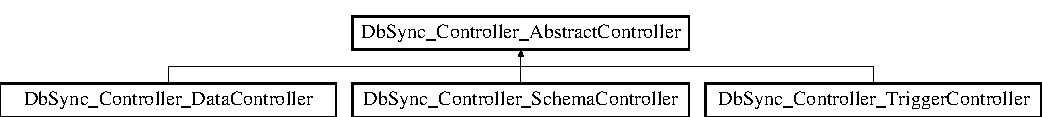
\includegraphics[height=1.568627cm]{classDbSync__Controller__AbstractController}
\end{center}
\end{figure}
\subsection*{Public Member Functions}
\begin{DoxyCompactItemize}
\item 
\hyperlink{classDbSync__Controller__AbstractController_a6afb890b457d835ce2fc37177a73268c}{\_\-\_\-construct} (array \$config)
\item 
\hyperlink{classDbSync__Controller__AbstractController_a26c95d326895bcad46f6b61a3674f5c6}{dispatch} (\hyperlink{classDbSync__Console}{DbSync\_\-Console} \$console)
\item 
\hyperlink{classDbSync__Controller__AbstractController_ac07432b2dbe3854b4f7924fa7887215c}{getItemsList} (\$action)
\item 
\hyperlink{classDbSync__Controller__AbstractController_a40107b1c2a0d5e2f3da236a5c32c2f93}{\_\-\_\-destruct} ()
\item 
\hyperlink{classDbSync__Controller__AbstractController_aaffa31e72a2dcdd6d2a144b8000e7231}{helpAction} ()
\item 
\hyperlink{classDbSync__Controller__AbstractController_aa27d714cc779879c43ca3621c65c65de}{showUsage} ()
\item 
\hyperlink{classDbSync__Controller__AbstractController_a12b74400d214770030c52d2f29308f52}{statusAction} ()
\item 
\hyperlink{classDbSync__Controller__AbstractController_ae973fdc065acffa90f43425b2d480794}{initAction} ()
\item 
\hyperlink{classDbSync__Controller__AbstractController_ab0e568570a013d19ba46b44c4e1e4aa4}{pullAction} ()
\item 
\hyperlink{classDbSync__Controller__AbstractController_a94bd514ad322a37bf6bf2158b98b69b7}{diffAction} ()
\item 
\hyperlink{classDbSync__Controller__AbstractController_abcec7de3ac2e1a43ff35ec2190a9c8d3}{colorize} (\$text, \$color= 'yellow')
\end{DoxyCompactItemize}
\subsection*{Protected Member Functions}
\begin{DoxyCompactItemize}
\item 
\hyperlink{classDbSync__Controller__AbstractController_ae7f065286125487dd51f268138c02113}{\_\-run} (\$action, \$name)
\end{DoxyCompactItemize}
\subsection*{Protected Attributes}
\begin{DoxyCompactItemize}
\item 
\hypertarget{classDbSync__Controller__AbstractController_a419e0e008929c4ac2294a6f90c5965b3}{
{\bfseries \$\_\-modelClass}}
\label{classDbSync__Controller__AbstractController_a419e0e008929c4ac2294a6f90c5965b3}

\item 
\hypertarget{classDbSync__Controller__AbstractController_a499e13fe1d21e988cccccf5497dc0003}{
{\bfseries \$\_\-model}}
\label{classDbSync__Controller__AbstractController_a499e13fe1d21e988cccccf5497dc0003}

\item 
\hypertarget{classDbSync__Controller__AbstractController_a6bd7ca3e9e3faf8da55701916ca82b31}{
{\bfseries \$\_\-console}}
\label{classDbSync__Controller__AbstractController_a6bd7ca3e9e3faf8da55701916ca82b31}

\end{DoxyCompactItemize}


\subsection{Constructor \& Destructor Documentation}
\hypertarget{classDbSync__Controller__AbstractController_a6afb890b457d835ce2fc37177a73268c}{
\index{DbSync\_\-Controller\_\-AbstractController@{DbSync\_\-Controller\_\-AbstractController}!\_\-\_\-construct@{\_\-\_\-construct}}
\index{\_\-\_\-construct@{\_\-\_\-construct}!DbSync_Controller_AbstractController@{DbSync\_\-Controller\_\-AbstractController}}
\subsubsection[{\_\-\_\-construct}]{\setlength{\rightskip}{0pt plus 5cm}DbSync\_\-Controller\_\-AbstractController::\_\-\_\-construct (
\begin{DoxyParamCaption}
\item[{array \$}]{config}
\end{DoxyParamCaption}
)}}
\label{classDbSync__Controller__AbstractController_a6afb890b457d835ce2fc37177a73268c}
Constructor


\begin{DoxyParams}[1]{Parameters}
array & {\em \$config} & \\
\hline
\end{DoxyParams}
\hypertarget{classDbSync__Controller__AbstractController_a40107b1c2a0d5e2f3da236a5c32c2f93}{
\index{DbSync\_\-Controller\_\-AbstractController@{DbSync\_\-Controller\_\-AbstractController}!\_\-\_\-destruct@{\_\-\_\-destruct}}
\index{\_\-\_\-destruct@{\_\-\_\-destruct}!DbSync_Controller_AbstractController@{DbSync\_\-Controller\_\-AbstractController}}
\subsubsection[{\_\-\_\-destruct}]{\setlength{\rightskip}{0pt plus 5cm}DbSync\_\-Controller\_\-AbstractController::\_\-\_\-destruct (
\begin{DoxyParamCaption}
{}
\end{DoxyParamCaption}
)}}
\label{classDbSync__Controller__AbstractController_a40107b1c2a0d5e2f3da236a5c32c2f93}
Descructor 

\subsection{Member Function Documentation}
\hypertarget{classDbSync__Controller__AbstractController_ae7f065286125487dd51f268138c02113}{
\index{DbSync\_\-Controller\_\-AbstractController@{DbSync\_\-Controller\_\-AbstractController}!\_\-run@{\_\-run}}
\index{\_\-run@{\_\-run}!DbSync_Controller_AbstractController@{DbSync\_\-Controller\_\-AbstractController}}
\subsubsection[{\_\-run}]{\setlength{\rightskip}{0pt plus 5cm}DbSync\_\-Controller\_\-AbstractController::\_\-run (
\begin{DoxyParamCaption}
\item[{\$}]{action, }
\item[{\$}]{name}
\end{DoxyParamCaption}
)\hspace{0.3cm}{\ttfamily  \mbox{[}protected\mbox{]}}}}
\label{classDbSync__Controller__AbstractController_ae7f065286125487dd51f268138c02113}
Run action


\begin{DoxyParams}[1]{Parameters}
string & {\em \$action} & \\
\hline
string & {\em \$name} & \\
\hline
\end{DoxyParams}


Reimplemented in \hyperlink{classDbSync__Controller__TriggerController_a2b8ff414b903fc7ac1a433d1f10e2b5a}{DbSync\_\-Controller\_\-TriggerController}.

\hypertarget{classDbSync__Controller__AbstractController_abcec7de3ac2e1a43ff35ec2190a9c8d3}{
\index{DbSync\_\-Controller\_\-AbstractController@{DbSync\_\-Controller\_\-AbstractController}!colorize@{colorize}}
\index{colorize@{colorize}!DbSync_Controller_AbstractController@{DbSync\_\-Controller\_\-AbstractController}}
\subsubsection[{colorize}]{\setlength{\rightskip}{0pt plus 5cm}DbSync\_\-Controller\_\-AbstractController::colorize (
\begin{DoxyParamCaption}
\item[{\$}]{text, }
\item[{\$}]{color = {\ttfamily 'yellow'}}
\end{DoxyParamCaption}
)}}
\label{classDbSync__Controller__AbstractController_abcec7de3ac2e1a43ff35ec2190a9c8d3}
Colorize


\begin{DoxyParams}[1]{Parameters}
string & {\em \$text} & \\
\hline
string & {\em \$color} & \\
\hline
\end{DoxyParams}
\begin{DoxyReturn}{Returns}
string 
\end{DoxyReturn}
\hypertarget{classDbSync__Controller__AbstractController_a94bd514ad322a37bf6bf2158b98b69b7}{
\index{DbSync\_\-Controller\_\-AbstractController@{DbSync\_\-Controller\_\-AbstractController}!diffAction@{diffAction}}
\index{diffAction@{diffAction}!DbSync_Controller_AbstractController@{DbSync\_\-Controller\_\-AbstractController}}
\subsubsection[{diffAction}]{\setlength{\rightskip}{0pt plus 5cm}DbSync\_\-Controller\_\-AbstractController::diffAction (
\begin{DoxyParamCaption}
{}
\end{DoxyParamCaption}
)}}
\label{classDbSync__Controller__AbstractController_a94bd514ad322a37bf6bf2158b98b69b7}
Diff

\begin{DoxyReturn}{Returns}
Show diff between database table schema and schema config file 
\end{DoxyReturn}


Reimplemented in \hyperlink{classDbSync__Controller__TriggerController_a485f3483de2efad7b59b9cb5cef694b4}{DbSync\_\-Controller\_\-TriggerController}.

\hypertarget{classDbSync__Controller__AbstractController_a26c95d326895bcad46f6b61a3674f5c6}{
\index{DbSync\_\-Controller\_\-AbstractController@{DbSync\_\-Controller\_\-AbstractController}!dispatch@{dispatch}}
\index{dispatch@{dispatch}!DbSync_Controller_AbstractController@{DbSync\_\-Controller\_\-AbstractController}}
\subsubsection[{dispatch}]{\setlength{\rightskip}{0pt plus 5cm}DbSync\_\-Controller\_\-AbstractController::dispatch (
\begin{DoxyParamCaption}
\item[{{\bf DbSync\_\-Console} \$}]{console}
\end{DoxyParamCaption}
)}}
\label{classDbSync__Controller__AbstractController_a26c95d326895bcad46f6b61a3674f5c6}
Dispatch


\begin{DoxyParams}[1]{Parameters}
\hyperlink{classDbSync__Console}{DbSync\_\-Console} & {\em \$console} & \\
\hline
\end{DoxyParams}
\begin{DoxyReturn}{Returns}
mixed 
\end{DoxyReturn}
\hypertarget{classDbSync__Controller__AbstractController_ac07432b2dbe3854b4f7924fa7887215c}{
\index{DbSync\_\-Controller\_\-AbstractController@{DbSync\_\-Controller\_\-AbstractController}!getItemsList@{getItemsList}}
\index{getItemsList@{getItemsList}!DbSync_Controller_AbstractController@{DbSync\_\-Controller\_\-AbstractController}}
\subsubsection[{getItemsList}]{\setlength{\rightskip}{0pt plus 5cm}DbSync\_\-Controller\_\-AbstractController::getItemsList (
\begin{DoxyParamCaption}
\item[{\$}]{action}
\end{DoxyParamCaption}
)}}
\label{classDbSync__Controller__AbstractController_ac07432b2dbe3854b4f7924fa7887215c}
Get items list


\begin{DoxyParams}[1]{Parameters}
string & {\em \$action} & \\
\hline
\end{DoxyParams}
\begin{DoxyReturn}{Returns}
array 
\end{DoxyReturn}


Reimplemented in \hyperlink{classDbSync__Controller__TriggerController_a18f4eb165243504cf1354464be4ec9de}{DbSync\_\-Controller\_\-TriggerController}.

\hypertarget{classDbSync__Controller__AbstractController_aaffa31e72a2dcdd6d2a144b8000e7231}{
\index{DbSync\_\-Controller\_\-AbstractController@{DbSync\_\-Controller\_\-AbstractController}!helpAction@{helpAction}}
\index{helpAction@{helpAction}!DbSync_Controller_AbstractController@{DbSync\_\-Controller\_\-AbstractController}}
\subsubsection[{helpAction}]{\setlength{\rightskip}{0pt plus 5cm}DbSync\_\-Controller\_\-AbstractController::helpAction (
\begin{DoxyParamCaption}
{}
\end{DoxyParamCaption}
)}}
\label{classDbSync__Controller__AbstractController_aaffa31e72a2dcdd6d2a144b8000e7231}
Help action

\begin{DoxyReturn}{Returns}
Help message 
\end{DoxyReturn}


Reimplemented in \hyperlink{classDbSync__Controller__TriggerController_a4d53a691eb15f7d060c4db5d14e8c240}{DbSync\_\-Controller\_\-TriggerController}.

\hypertarget{classDbSync__Controller__AbstractController_ae973fdc065acffa90f43425b2d480794}{
\index{DbSync\_\-Controller\_\-AbstractController@{DbSync\_\-Controller\_\-AbstractController}!initAction@{initAction}}
\index{initAction@{initAction}!DbSync_Controller_AbstractController@{DbSync\_\-Controller\_\-AbstractController}}
\subsubsection[{initAction}]{\setlength{\rightskip}{0pt plus 5cm}DbSync\_\-Controller\_\-AbstractController::initAction (
\begin{DoxyParamCaption}
{}
\end{DoxyParamCaption}
)}}
\label{classDbSync__Controller__AbstractController_ae973fdc065acffa90f43425b2d480794}
Init

\begin{DoxyReturn}{Returns}
Create config file(s) 
\end{DoxyReturn}


Reimplemented in \hyperlink{classDbSync__Controller__TriggerController_ac5ee83f5159f52d4327632347a25c2dd}{DbSync\_\-Controller\_\-TriggerController}.

\hypertarget{classDbSync__Controller__AbstractController_ab0e568570a013d19ba46b44c4e1e4aa4}{
\index{DbSync\_\-Controller\_\-AbstractController@{DbSync\_\-Controller\_\-AbstractController}!pullAction@{pullAction}}
\index{pullAction@{pullAction}!DbSync_Controller_AbstractController@{DbSync\_\-Controller\_\-AbstractController}}
\subsubsection[{pullAction}]{\setlength{\rightskip}{0pt plus 5cm}DbSync\_\-Controller\_\-AbstractController::pullAction (
\begin{DoxyParamCaption}
{}
\end{DoxyParamCaption}
)}}
\label{classDbSync__Controller__AbstractController_ab0e568570a013d19ba46b44c4e1e4aa4}
Pull

\begin{DoxyReturn}{Returns}
Override current table config(s) file by new created from database 
\end{DoxyReturn}


Reimplemented in \hyperlink{classDbSync__Controller__TriggerController_ada505e291b61976b9a9a8b3a1b64e998}{DbSync\_\-Controller\_\-TriggerController}.

\hypertarget{classDbSync__Controller__AbstractController_aa27d714cc779879c43ca3621c65c65de}{
\index{DbSync\_\-Controller\_\-AbstractController@{DbSync\_\-Controller\_\-AbstractController}!showUsage@{showUsage}}
\index{showUsage@{showUsage}!DbSync_Controller_AbstractController@{DbSync\_\-Controller\_\-AbstractController}}
\subsubsection[{showUsage}]{\setlength{\rightskip}{0pt plus 5cm}DbSync\_\-Controller\_\-AbstractController::showUsage (
\begin{DoxyParamCaption}
{}
\end{DoxyParamCaption}
)}}
\label{classDbSync__Controller__AbstractController_aa27d714cc779879c43ca3621c65c65de}
Output actions usage message \hypertarget{classDbSync__Controller__AbstractController_a12b74400d214770030c52d2f29308f52}{
\index{DbSync\_\-Controller\_\-AbstractController@{DbSync\_\-Controller\_\-AbstractController}!statusAction@{statusAction}}
\index{statusAction@{statusAction}!DbSync_Controller_AbstractController@{DbSync\_\-Controller\_\-AbstractController}}
\subsubsection[{statusAction}]{\setlength{\rightskip}{0pt plus 5cm}DbSync\_\-Controller\_\-AbstractController::statusAction (
\begin{DoxyParamCaption}
{}
\end{DoxyParamCaption}
)}}
\label{classDbSync__Controller__AbstractController_a12b74400d214770030c52d2f29308f52}
Status

\begin{DoxyReturn}{Returns}
Check sync status (Ok/Unsyncronized) 
\end{DoxyReturn}


Reimplemented in \hyperlink{classDbSync__Controller__TriggerController_a08d8439a825dd363b7fb8df076056f65}{DbSync\_\-Controller\_\-TriggerController}.



The documentation for this class was generated from the following file:\begin{DoxyCompactItemize}
\item 
DbSync/Controller/AbstractController.php\end{DoxyCompactItemize}

\hypertarget{classDbSync__Controller__DataController}{
\section{DbSync\_\-Controller\_\-DataController Class Reference}
\label{classDbSync__Controller__DataController}\index{DbSync\_\-Controller\_\-DataController@{DbSync\_\-Controller\_\-DataController}}
}
Inheritance diagram for DbSync\_\-Controller\_\-DataController:\begin{figure}[H]
\begin{center}
\leavevmode
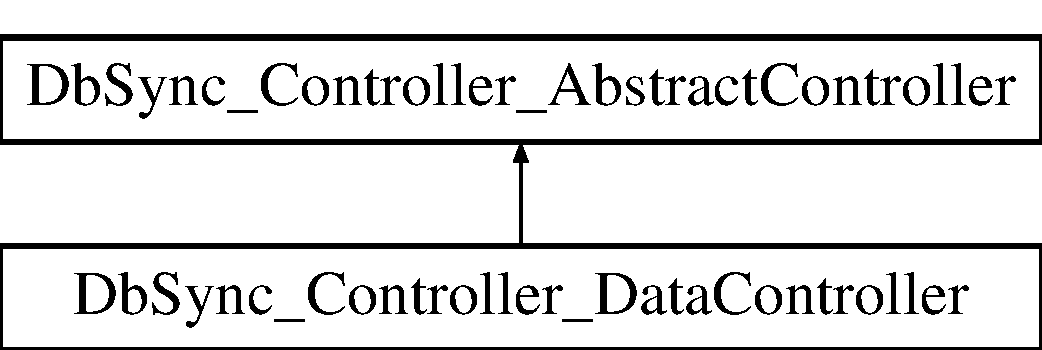
\includegraphics[height=2.000000cm]{classDbSync__Controller__DataController}
\end{center}
\end{figure}
\subsection*{Public Member Functions}
\begin{DoxyCompactItemize}
\item 
\hyperlink{classDbSync__Controller__DataController_a905f98b976e7fa950805cb40f569cbc9}{pushAction} ()
\item 
\hyperlink{classDbSync__Controller__DataController_af83b5323b69423e094c82d965eb72b31}{mergeAction} ()
\end{DoxyCompactItemize}
\subsection*{Protected Attributes}
\begin{DoxyCompactItemize}
\item 
\hypertarget{classDbSync__Controller__DataController_a0ca5fd39aa4db5536a05b5acfcf0d6f9}{
{\bfseries \$\_\-modelClass} = '\hyperlink{classDbSync__Table__Data}{DbSync\_\-Table\_\-Data}'}
\label{classDbSync__Controller__DataController_a0ca5fd39aa4db5536a05b5acfcf0d6f9}

\end{DoxyCompactItemize}


\subsection{Member Function Documentation}
\hypertarget{classDbSync__Controller__DataController_af83b5323b69423e094c82d965eb72b31}{
\index{DbSync\_\-Controller\_\-DataController@{DbSync\_\-Controller\_\-DataController}!mergeAction@{mergeAction}}
\index{mergeAction@{mergeAction}!DbSync_Controller_DataController@{DbSync\_\-Controller\_\-DataController}}
\subsubsection[{mergeAction}]{\setlength{\rightskip}{0pt plus 5cm}DbSync\_\-Controller\_\-DataController::mergeAction (
\begin{DoxyParamCaption}
{}
\end{DoxyParamCaption}
)}}
\label{classDbSync__Controller__DataController_af83b5323b69423e094c82d965eb72b31}
Merge

\begin{DoxyReturn}{Returns}
Merge data rows from config file to database table 
\end{DoxyReturn}
\hypertarget{classDbSync__Controller__DataController_a905f98b976e7fa950805cb40f569cbc9}{
\index{DbSync\_\-Controller\_\-DataController@{DbSync\_\-Controller\_\-DataController}!pushAction@{pushAction}}
\index{pushAction@{pushAction}!DbSync_Controller_DataController@{DbSync\_\-Controller\_\-DataController}}
\subsubsection[{pushAction}]{\setlength{\rightskip}{0pt plus 5cm}DbSync\_\-Controller\_\-DataController::pushAction (
\begin{DoxyParamCaption}
{}
\end{DoxyParamCaption}
)}}
\label{classDbSync__Controller__DataController_a905f98b976e7fa950805cb40f569cbc9}
Push

\begin{DoxyReturn}{Returns}
Override database data by current data config file 

Use \{-\/-\/force$|$yellow\} to truncate table first 
\end{DoxyReturn}


The documentation for this class was generated from the following file:\begin{DoxyCompactItemize}
\item 
DbSync/Controller/DataController.php\end{DoxyCompactItemize}

\hypertarget{classDbSync__Controller__SchemaController}{
\section{DbSync\_\-Controller\_\-SchemaController Class Reference}
\label{classDbSync__Controller__SchemaController}\index{DbSync\_\-Controller\_\-SchemaController@{DbSync\_\-Controller\_\-SchemaController}}
}
Inheritance diagram for DbSync\_\-Controller\_\-SchemaController:\begin{figure}[H]
\begin{center}
\leavevmode
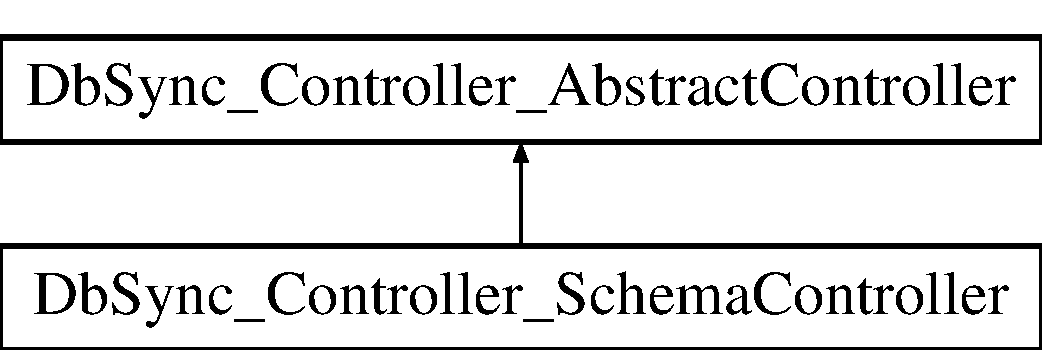
\includegraphics[height=2.000000cm]{classDbSync__Controller__SchemaController}
\end{center}
\end{figure}
\subsection*{Public Member Functions}
\begin{DoxyCompactItemize}
\item 
\hyperlink{classDbSync__Controller__SchemaController_abbd3a6e36859fdb8f8b0a849d284dc81}{deleteAction} ()
\end{DoxyCompactItemize}
\subsection*{Protected Attributes}
\begin{DoxyCompactItemize}
\item 
\hypertarget{classDbSync__Controller__SchemaController_a06640271494bac2c9177a2b87b8a8c13}{
{\bfseries \$\_\-modelClass} = '\hyperlink{classDbSync__Model__Table__Schema}{DbSync\_\-Model\_\-Table\_\-Schema}'}
\label{classDbSync__Controller__SchemaController_a06640271494bac2c9177a2b87b8a8c13}

\end{DoxyCompactItemize}


\subsection{Member Function Documentation}
\hypertarget{classDbSync__Controller__SchemaController_abbd3a6e36859fdb8f8b0a849d284dc81}{
\index{DbSync\_\-Controller\_\-SchemaController@{DbSync\_\-Controller\_\-SchemaController}!deleteAction@{deleteAction}}
\index{deleteAction@{deleteAction}!DbSync_Controller_SchemaController@{DbSync\_\-Controller\_\-SchemaController}}
\subsubsection[{deleteAction}]{\setlength{\rightskip}{0pt plus 5cm}DbSync\_\-Controller\_\-SchemaController::deleteAction (
\begin{DoxyParamCaption}
{}
\end{DoxyParamCaption}
)}}
\label{classDbSync__Controller__SchemaController_abbd3a6e36859fdb8f8b0a849d284dc81}
Delete

de

\begin{DoxyReturn}{Returns}
Delete table and config 

Use \{-\/-\/db$|$yellow\} to delete only form database 

Use \{-\/-\/file$|$yellow\} to delete only config file 
\end{DoxyReturn}


The documentation for this class was generated from the following file:\begin{DoxyCompactItemize}
\item 
DbSync/Controller/SchemaController.php\end{DoxyCompactItemize}

\hypertarget{classDbSync__Controller__TriggerController}{
\section{DbSync\_\-Controller\_\-TriggerController Class Reference}
\label{classDbSync__Controller__TriggerController}\index{DbSync\_\-Controller\_\-TriggerController@{DbSync\_\-Controller\_\-TriggerController}}
}
Inheritance diagram for DbSync\_\-Controller\_\-TriggerController:\begin{figure}[H]
\begin{center}
\leavevmode
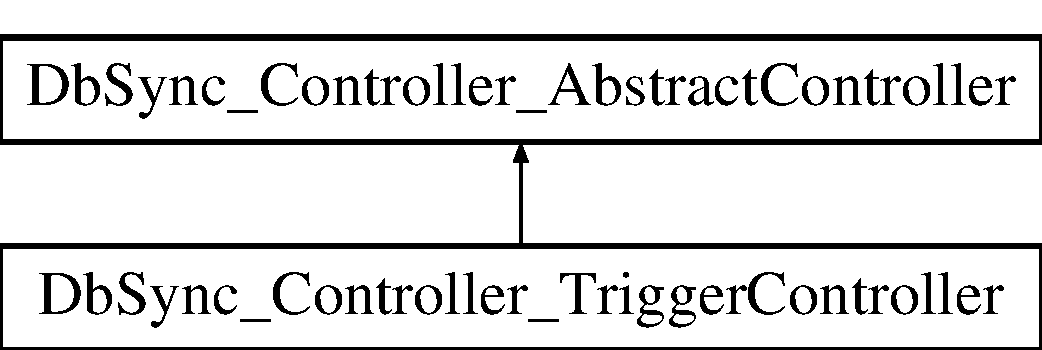
\includegraphics[height=2.000000cm]{classDbSync__Controller__TriggerController}
\end{center}
\end{figure}
\subsection*{Public Member Functions}
\begin{DoxyCompactItemize}
\item 
\hyperlink{classDbSync__Controller__TriggerController_a18f4eb165243504cf1354464be4ec9de}{getItemsList} (\$action)
\item 
\hyperlink{classDbSync__Controller__TriggerController_a4d53a691eb15f7d060c4db5d14e8c240}{helpAction} ()
\item 
\hyperlink{classDbSync__Controller__TriggerController_af0518cd0c76d9ae0a20b44d2a1c311b0}{deleteAction} ()
\item 
\hyperlink{classDbSync__Controller__TriggerController_a08d8439a825dd363b7fb8df076056f65}{statusAction} ()
\end{DoxyCompactItemize}
\subsection*{Protected Member Functions}
\begin{DoxyCompactItemize}
\item 
\hyperlink{classDbSync__Controller__TriggerController_a2b8ff414b903fc7ac1a433d1f10e2b5a}{\_\-run} (\$action, \$name)
\end{DoxyCompactItemize}
\subsection*{Protected Attributes}
\begin{DoxyCompactItemize}
\item 
\hypertarget{classDbSync__Controller__TriggerController_a9e3a9ae192647f811cb45f77e97af78d}{
{\bfseries \$\_\-modelClass} = '\hyperlink{classDbSync__Model__Table__Trigger}{DbSync\_\-Model\_\-Table\_\-Trigger}'}
\label{classDbSync__Controller__TriggerController_a9e3a9ae192647f811cb45f77e97af78d}

\item 
\hypertarget{classDbSync__Controller__TriggerController_a5b69850f05d66f66508a58bf60ee1378}{
{\bfseries \$\_\-model}}
\label{classDbSync__Controller__TriggerController_a5b69850f05d66f66508a58bf60ee1378}

\end{DoxyCompactItemize}


\subsection{Member Function Documentation}
\hypertarget{classDbSync__Controller__TriggerController_a2b8ff414b903fc7ac1a433d1f10e2b5a}{
\index{DbSync\_\-Controller\_\-TriggerController@{DbSync\_\-Controller\_\-TriggerController}!\_\-run@{\_\-run}}
\index{\_\-run@{\_\-run}!DbSync_Controller_TriggerController@{DbSync\_\-Controller\_\-TriggerController}}
\subsubsection[{\_\-run}]{\setlength{\rightskip}{0pt plus 5cm}DbSync\_\-Controller\_\-TriggerController::\_\-run (
\begin{DoxyParamCaption}
\item[{\$}]{action, }
\item[{\$}]{name}
\end{DoxyParamCaption}
)\hspace{0.3cm}{\ttfamily  \mbox{[}protected\mbox{]}}}}
\label{classDbSync__Controller__TriggerController_a2b8ff414b903fc7ac1a433d1f10e2b5a}
Run action


\begin{DoxyParams}[1]{Parameters}
string & {\em \$action} & \\
\hline
string & {\em \$name} & \\
\hline
\end{DoxyParams}


Reimplemented from \hyperlink{classDbSync__Controller__AbstractController_ae7f065286125487dd51f268138c02113}{DbSync\_\-Controller\_\-AbstractController}.

\hypertarget{classDbSync__Controller__TriggerController_af0518cd0c76d9ae0a20b44d2a1c311b0}{
\index{DbSync\_\-Controller\_\-TriggerController@{DbSync\_\-Controller\_\-TriggerController}!deleteAction@{deleteAction}}
\index{deleteAction@{deleteAction}!DbSync_Controller_TriggerController@{DbSync\_\-Controller\_\-TriggerController}}
\subsubsection[{deleteAction}]{\setlength{\rightskip}{0pt plus 5cm}DbSync\_\-Controller\_\-TriggerController::deleteAction (
\begin{DoxyParamCaption}
{}
\end{DoxyParamCaption}
)}}
\label{classDbSync__Controller__TriggerController_af0518cd0c76d9ae0a20b44d2a1c311b0}
Delete

de

\begin{DoxyReturn}{Returns}
Delete trigger and config 

Use \{-\/-\/db$|$yellow\} to delete only from database 

Use \{-\/-\/file$|$yellow\} to delete only config file 
\end{DoxyReturn}
\hypertarget{classDbSync__Controller__TriggerController_a18f4eb165243504cf1354464be4ec9de}{
\index{DbSync\_\-Controller\_\-TriggerController@{DbSync\_\-Controller\_\-TriggerController}!getItemsList@{getItemsList}}
\index{getItemsList@{getItemsList}!DbSync_Controller_TriggerController@{DbSync\_\-Controller\_\-TriggerController}}
\subsubsection[{getItemsList}]{\setlength{\rightskip}{0pt plus 5cm}DbSync\_\-Controller\_\-TriggerController::getItemsList (
\begin{DoxyParamCaption}
\item[{\$}]{action}
\end{DoxyParamCaption}
)}}
\label{classDbSync__Controller__TriggerController_a18f4eb165243504cf1354464be4ec9de}
Get items list


\begin{DoxyParams}[1]{Parameters}
string & {\em \$action} & \\
\hline
\end{DoxyParams}
\begin{DoxyReturn}{Returns}
array 
\end{DoxyReturn}


Reimplemented from \hyperlink{classDbSync__Controller__AbstractController_ac07432b2dbe3854b4f7924fa7887215c}{DbSync\_\-Controller\_\-AbstractController}.

\hypertarget{classDbSync__Controller__TriggerController_a4d53a691eb15f7d060c4db5d14e8c240}{
\index{DbSync\_\-Controller\_\-TriggerController@{DbSync\_\-Controller\_\-TriggerController}!helpAction@{helpAction}}
\index{helpAction@{helpAction}!DbSync_Controller_TriggerController@{DbSync\_\-Controller\_\-TriggerController}}
\subsubsection[{helpAction}]{\setlength{\rightskip}{0pt plus 5cm}DbSync\_\-Controller\_\-TriggerController::helpAction (
\begin{DoxyParamCaption}
{}
\end{DoxyParamCaption}
)}}
\label{classDbSync__Controller__TriggerController_a4d53a691eb15f7d060c4db5d14e8c240}
Help

\begin{DoxyReturn}{Returns}
Help message 
\end{DoxyReturn}
\begin{DoxySeeAlso}{See also}
DbSync\_\-Controller::help() 
\end{DoxySeeAlso}


Reimplemented from \hyperlink{classDbSync__Controller__AbstractController_aaffa31e72a2dcdd6d2a144b8000e7231}{DbSync\_\-Controller\_\-AbstractController}.

\hypertarget{classDbSync__Controller__TriggerController_a08d8439a825dd363b7fb8df076056f65}{
\index{DbSync\_\-Controller\_\-TriggerController@{DbSync\_\-Controller\_\-TriggerController}!statusAction@{statusAction}}
\index{statusAction@{statusAction}!DbSync_Controller_TriggerController@{DbSync\_\-Controller\_\-TriggerController}}
\subsubsection[{statusAction}]{\setlength{\rightskip}{0pt plus 5cm}DbSync\_\-Controller\_\-TriggerController::statusAction (
\begin{DoxyParamCaption}
{}
\end{DoxyParamCaption}
)}}
\label{classDbSync__Controller__TriggerController_a08d8439a825dd363b7fb8df076056f65}
Status

st

\begin{DoxyReturn}{Returns}
Check triggers status (Ok/Unsyncronized) 

Use \{-\/-\/table \mbox{[}\mbox{[}tableName\mbox{]} ... \mbox{]}$|$yellow\} to display triggers for certain table(s) 
\end{DoxyReturn}


Reimplemented from \hyperlink{classDbSync__Controller__AbstractController_a12b74400d214770030c52d2f29308f52}{DbSync\_\-Controller\_\-AbstractController}.



The documentation for this class was generated from the following file:\begin{DoxyCompactItemize}
\item 
DbSync/Controller/TriggerController.php\end{DoxyCompactItemize}

\hypertarget{classDbSync__Exception}{
\section{DbSync\_\-Exception Class Reference}
\label{classDbSync__Exception}\index{DbSync\_\-Exception@{DbSync\_\-Exception}}
}


The documentation for this class was generated from the following file:\begin{DoxyCompactItemize}
\item 
DbSync/Exception.php\end{DoxyCompactItemize}

\hypertarget{classDbSync__Table__AbstractTable}{
\section{DbSync\_\-Table\_\-AbstractTable Class Reference}
\label{classDbSync__Table__AbstractTable}\index{DbSync\_\-Table\_\-AbstractTable@{DbSync\_\-Table\_\-AbstractTable}}
}
Inheritance diagram for DbSync\_\-Table\_\-AbstractTable:\begin{figure}[H]
\begin{center}
\leavevmode
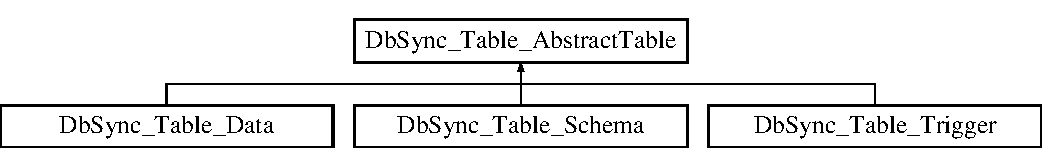
\includegraphics[height=1.985816cm]{classDbSync__Table__AbstractTable}
\end{center}
\end{figure}
\subsection*{Public Member Functions}
\begin{DoxyCompactItemize}
\item 
\hyperlink{classDbSync__Table__AbstractTable_a7be38fca9d01a74c007366439d7ed3cf}{\_\-\_\-construct} (\hyperlink{interfaceDbSync__Table__DbAdapter__AdapterInterface}{DbSync\_\-Table\_\-DbAdapter\_\-AdapterInterface} \$db, \hyperlink{interfaceDbSync__Table__FileAdapter__AdapterInterface}{DbSync\_\-Table\_\-FileAdapter\_\-AdapterInterface} \$file, \$diffProg=null)
\item 
\hyperlink{classDbSync__Table__AbstractTable_a602dcefdf77e6469d86640398fcc6f3e}{setDiffProg} (\$diffProg)
\item 
\hyperlink{classDbSync__Table__AbstractTable_a73bb91b00d38f9653f822ce5f22fdc85}{getTableName} ()
\item 
\hyperlink{classDbSync__Table__AbstractTable_ab404bd1cdfb4ff587049ddaa763bbdfc}{setTableName} (\$tableName)
\item 
\hyperlink{classDbSync__Table__AbstractTable_a6c761e01599281f6d057094e00e40c8a}{save} (\$filename)
\item 
\hyperlink{classDbSync__Table__AbstractTable_a57772ff792f746e80ed34375ab2c7953}{isWriteable} ()
\item 
\hyperlink{classDbSync__Table__AbstractTable_a7185ca51ac03d3c30225ec350dab000d}{getListDb} ()
\item 
\hyperlink{classDbSync__Table__AbstractTable_ab650d6290afb12319a792eafb844db80}{getListConfig} ()
\item 
\hyperlink{classDbSync__Table__AbstractTable_a883d73aa5b5f30db79172c7934e28ddc}{getList} ()
\item 
\hyperlink{classDbSync__Table__AbstractTable_a247c6ebe39888ce659265e90701ad66d}{hasDbTable} ()
\item 
\hyperlink{classDbSync__Table__AbstractTable_a69d854fa880beb9ce0a589e0e604c78d}{getFilePath} (\$real=true)
\item 
\hyperlink{classDbSync__Table__AbstractTable_a4129bcdf6e1caaae2f2a2f27471a66a6}{hasFile} ()
\item 
\hyperlink{classDbSync__Table__AbstractTable_a5633ace9bdfd4f6b0d1b6498492e8be8}{deleteFile} ()
\item 
\hyperlink{classDbSync__Table__AbstractTable_a3c98d38cfab450c5df4c7f74ab0054e5}{getStatus} ()
\item 
\hyperlink{classDbSync__Table__AbstractTable_a6d18b62e3ba05af99b5ae0f57f3d6f6b}{pull} ()
\item 
\hyperlink{classDbSync__Table__AbstractTable_a77fdfb2eb8a96c4d646bbf756d9ab9ce}{diff} ()
\item 
\hyperlink{classDbSync__Table__AbstractTable_abaa8cce0accbd902cc0ae32597e4966d}{init} (\$force=false)
\end{DoxyCompactItemize}
\subsection*{Protected Attributes}
\begin{DoxyCompactItemize}
\item 
\hypertarget{classDbSync__Table__AbstractTable_a0e14495b94bf28c946d7a358e451a0d9}{
{\bfseries \$\_\-dbAdapter}}
\label{classDbSync__Table__AbstractTable_a0e14495b94bf28c946d7a358e451a0d9}

\item 
\hypertarget{classDbSync__Table__AbstractTable_a54ff364459ce786ed1dde39a13b23ab9}{
{\bfseries \$\_\-fileAdapter}}
\label{classDbSync__Table__AbstractTable_a54ff364459ce786ed1dde39a13b23ab9}

\item 
\hypertarget{classDbSync__Table__AbstractTable_ad4b3983a04ca622b1fa53e5ae3572435}{
{\bfseries \$\_\-tableName}}
\label{classDbSync__Table__AbstractTable_ad4b3983a04ca622b1fa53e5ae3572435}

\item 
\hypertarget{classDbSync__Table__AbstractTable_a2a27a2cdcde4195d49b8a211b2748996}{
{\bfseries \$\_\-filename}}
\label{classDbSync__Table__AbstractTable_a2a27a2cdcde4195d49b8a211b2748996}

\item 
\hypertarget{classDbSync__Table__AbstractTable_ac9bdb64a866b5bcaa950f85c917bf655}{
{\bfseries \$\_\-diff} = 'diff'}
\label{classDbSync__Table__AbstractTable_ac9bdb64a866b5bcaa950f85c917bf655}

\item 
\hypertarget{classDbSync__Table__AbstractTable_aed634c197397fa86a615ba45845bf0d2}{
{\bfseries \$\_\-exceptionClass} = '\hyperlink{classDbSync__Exception}{DbSync\_\-Exception}'}
\label{classDbSync__Table__AbstractTable_aed634c197397fa86a615ba45845bf0d2}

\end{DoxyCompactItemize}


\subsection{Constructor \& Destructor Documentation}
\hypertarget{classDbSync__Table__AbstractTable_a7be38fca9d01a74c007366439d7ed3cf}{
\index{DbSync\_\-Table\_\-AbstractTable@{DbSync\_\-Table\_\-AbstractTable}!\_\-\_\-construct@{\_\-\_\-construct}}
\index{\_\-\_\-construct@{\_\-\_\-construct}!DbSync_Table_AbstractTable@{DbSync\_\-Table\_\-AbstractTable}}
\subsubsection[{\_\-\_\-construct}]{\setlength{\rightskip}{0pt plus 5cm}DbSync\_\-Table\_\-AbstractTable::\_\-\_\-construct (
\begin{DoxyParamCaption}
\item[{{\bf DbSync\_\-Table\_\-DbAdapter\_\-AdapterInterface} \$}]{db, }
\item[{{\bf DbSync\_\-Table\_\-FileAdapter\_\-AdapterInterface} \$}]{file, }
\item[{\$}]{diffProg = {\ttfamily null}}
\end{DoxyParamCaption}
)}}
\label{classDbSync__Table__AbstractTable_a7be38fca9d01a74c007366439d7ed3cf}
Constructor


\begin{DoxyParams}[1]{Parameters}
\hyperlink{interfaceDbSync__Table__DbAdapter__AdapterInterface}{DbSync\_\-Table\_\-DbAdapter\_\-AdapterInterface} & {\em \$db} & \\
\hline
\hyperlink{interfaceDbSync__Table__FileAdapter__AdapterInterface}{DbSync\_\-Table\_\-FileAdapter\_\-AdapterInterface} & {\em \$file} & \\
\hline
string & {\em \$diffProg} & \\
\hline
\end{DoxyParams}


\subsection{Member Function Documentation}
\hypertarget{classDbSync__Table__AbstractTable_a5633ace9bdfd4f6b0d1b6498492e8be8}{
\index{DbSync\_\-Table\_\-AbstractTable@{DbSync\_\-Table\_\-AbstractTable}!deleteFile@{deleteFile}}
\index{deleteFile@{deleteFile}!DbSync_Table_AbstractTable@{DbSync\_\-Table\_\-AbstractTable}}
\subsubsection[{deleteFile}]{\setlength{\rightskip}{0pt plus 5cm}DbSync\_\-Table\_\-AbstractTable::deleteFile (
\begin{DoxyParamCaption}
{}
\end{DoxyParamCaption}
)}}
\label{classDbSync__Table__AbstractTable_a5633ace9bdfd4f6b0d1b6498492e8be8}
Delete file


\begin{DoxyExceptions}{Exceptions}
{\em Exception} & \\
\hline
\end{DoxyExceptions}
\begin{DoxyReturn}{Returns}
boolen 
\end{DoxyReturn}
\hypertarget{classDbSync__Table__AbstractTable_a77fdfb2eb8a96c4d646bbf756d9ab9ce}{
\index{DbSync\_\-Table\_\-AbstractTable@{DbSync\_\-Table\_\-AbstractTable}!diff@{diff}}
\index{diff@{diff}!DbSync_Table_AbstractTable@{DbSync\_\-Table\_\-AbstractTable}}
\subsubsection[{diff}]{\setlength{\rightskip}{0pt plus 5cm}DbSync\_\-Table\_\-AbstractTable::diff (
\begin{DoxyParamCaption}
{}
\end{DoxyParamCaption}
)}}
\label{classDbSync__Table__AbstractTable_a77fdfb2eb8a96c4d646bbf756d9ab9ce}
Get diff

\begin{DoxyReturn}{Returns}
array 
\end{DoxyReturn}
\hypertarget{classDbSync__Table__AbstractTable_a69d854fa880beb9ce0a589e0e604c78d}{
\index{DbSync\_\-Table\_\-AbstractTable@{DbSync\_\-Table\_\-AbstractTable}!getFilePath@{getFilePath}}
\index{getFilePath@{getFilePath}!DbSync_Table_AbstractTable@{DbSync\_\-Table\_\-AbstractTable}}
\subsubsection[{getFilePath}]{\setlength{\rightskip}{0pt plus 5cm}DbSync\_\-Table\_\-AbstractTable::getFilePath (
\begin{DoxyParamCaption}
\item[{\$}]{real = {\ttfamily true}}
\end{DoxyParamCaption}
)}}
\label{classDbSync__Table__AbstractTable_a69d854fa880beb9ce0a589e0e604c78d}
Get config filepath


\begin{DoxyParams}[1]{Parameters}
boolen & {\em \$real} & \\
\hline
\end{DoxyParams}

\begin{DoxyExceptions}{Exceptions}
{\em Exception} & \\
\hline
\end{DoxyExceptions}
\begin{DoxyReturn}{Returns}
string 
\end{DoxyReturn}


Reimplemented in \hyperlink{classDbSync__Table__Trigger_a56e0b413a1a52f79f639ba31fa857c55}{DbSync\_\-Table\_\-Trigger}.

\hypertarget{classDbSync__Table__AbstractTable_a883d73aa5b5f30db79172c7934e28ddc}{
\index{DbSync\_\-Table\_\-AbstractTable@{DbSync\_\-Table\_\-AbstractTable}!getList@{getList}}
\index{getList@{getList}!DbSync_Table_AbstractTable@{DbSync\_\-Table\_\-AbstractTable}}
\subsubsection[{getList}]{\setlength{\rightskip}{0pt plus 5cm}DbSync\_\-Table\_\-AbstractTable::getList (
\begin{DoxyParamCaption}
{}
\end{DoxyParamCaption}
)}}
\label{classDbSync__Table__AbstractTable_a883d73aa5b5f30db79172c7934e28ddc}
Get list

\begin{DoxyReturn}{Returns}
array 
\end{DoxyReturn}
\hypertarget{classDbSync__Table__AbstractTable_ab650d6290afb12319a792eafb844db80}{
\index{DbSync\_\-Table\_\-AbstractTable@{DbSync\_\-Table\_\-AbstractTable}!getListConfig@{getListConfig}}
\index{getListConfig@{getListConfig}!DbSync_Table_AbstractTable@{DbSync\_\-Table\_\-AbstractTable}}
\subsubsection[{getListConfig}]{\setlength{\rightskip}{0pt plus 5cm}DbSync\_\-Table\_\-AbstractTable::getListConfig (
\begin{DoxyParamCaption}
{}
\end{DoxyParamCaption}
)}}
\label{classDbSync__Table__AbstractTable_ab650d6290afb12319a792eafb844db80}
Get config tables list

\begin{DoxyReturn}{Returns}
array 
\end{DoxyReturn}
\hypertarget{classDbSync__Table__AbstractTable_a7185ca51ac03d3c30225ec350dab000d}{
\index{DbSync\_\-Table\_\-AbstractTable@{DbSync\_\-Table\_\-AbstractTable}!getListDb@{getListDb}}
\index{getListDb@{getListDb}!DbSync_Table_AbstractTable@{DbSync\_\-Table\_\-AbstractTable}}
\subsubsection[{getListDb}]{\setlength{\rightskip}{0pt plus 5cm}DbSync\_\-Table\_\-AbstractTable::getListDb (
\begin{DoxyParamCaption}
{}
\end{DoxyParamCaption}
)}}
\label{classDbSync__Table__AbstractTable_a7185ca51ac03d3c30225ec350dab000d}
Get db tables list

\begin{DoxyReturn}{Returns}
array 
\end{DoxyReturn}
\hypertarget{classDbSync__Table__AbstractTable_a3c98d38cfab450c5df4c7f74ab0054e5}{
\index{DbSync\_\-Table\_\-AbstractTable@{DbSync\_\-Table\_\-AbstractTable}!getStatus@{getStatus}}
\index{getStatus@{getStatus}!DbSync_Table_AbstractTable@{DbSync\_\-Table\_\-AbstractTable}}
\subsubsection[{getStatus}]{\setlength{\rightskip}{0pt plus 5cm}DbSync\_\-Table\_\-AbstractTable::getStatus (
\begin{DoxyParamCaption}
{}
\end{DoxyParamCaption}
)}}
\label{classDbSync__Table__AbstractTable_a3c98d38cfab450c5df4c7f74ab0054e5}
Get status

\begin{DoxyReturn}{Returns}
boolen 
\end{DoxyReturn}
\hypertarget{classDbSync__Table__AbstractTable_a73bb91b00d38f9653f822ce5f22fdc85}{
\index{DbSync\_\-Table\_\-AbstractTable@{DbSync\_\-Table\_\-AbstractTable}!getTableName@{getTableName}}
\index{getTableName@{getTableName}!DbSync_Table_AbstractTable@{DbSync\_\-Table\_\-AbstractTable}}
\subsubsection[{getTableName}]{\setlength{\rightskip}{0pt plus 5cm}DbSync\_\-Table\_\-AbstractTable::getTableName (
\begin{DoxyParamCaption}
{}
\end{DoxyParamCaption}
)}}
\label{classDbSync__Table__AbstractTable_a73bb91b00d38f9653f822ce5f22fdc85}
Get table name

\begin{DoxyReturn}{Returns}
string 
\end{DoxyReturn}


Reimplemented in \hyperlink{classDbSync__Table__Trigger_a2a4c13e2d99327751869644dc053ff85}{DbSync\_\-Table\_\-Trigger}.

\hypertarget{classDbSync__Table__AbstractTable_a247c6ebe39888ce659265e90701ad66d}{
\index{DbSync\_\-Table\_\-AbstractTable@{DbSync\_\-Table\_\-AbstractTable}!hasDbTable@{hasDbTable}}
\index{hasDbTable@{hasDbTable}!DbSync_Table_AbstractTable@{DbSync\_\-Table\_\-AbstractTable}}
\subsubsection[{hasDbTable}]{\setlength{\rightskip}{0pt plus 5cm}DbSync\_\-Table\_\-AbstractTable::hasDbTable (
\begin{DoxyParamCaption}
{}
\end{DoxyParamCaption}
)}}
\label{classDbSync__Table__AbstractTable_a247c6ebe39888ce659265e90701ad66d}
Is db table exists

\begin{DoxyReturn}{Returns}
boolen 
\end{DoxyReturn}
\hypertarget{classDbSync__Table__AbstractTable_a4129bcdf6e1caaae2f2a2f27471a66a6}{
\index{DbSync\_\-Table\_\-AbstractTable@{DbSync\_\-Table\_\-AbstractTable}!hasFile@{hasFile}}
\index{hasFile@{hasFile}!DbSync_Table_AbstractTable@{DbSync\_\-Table\_\-AbstractTable}}
\subsubsection[{hasFile}]{\setlength{\rightskip}{0pt plus 5cm}DbSync\_\-Table\_\-AbstractTable::hasFile (
\begin{DoxyParamCaption}
{}
\end{DoxyParamCaption}
)}}
\label{classDbSync__Table__AbstractTable_a4129bcdf6e1caaae2f2a2f27471a66a6}
Has file

\begin{DoxyReturn}{Returns}
boolen 
\end{DoxyReturn}
\hypertarget{classDbSync__Table__AbstractTable_abaa8cce0accbd902cc0ae32597e4966d}{
\index{DbSync\_\-Table\_\-AbstractTable@{DbSync\_\-Table\_\-AbstractTable}!init@{init}}
\index{init@{init}!DbSync_Table_AbstractTable@{DbSync\_\-Table\_\-AbstractTable}}
\subsubsection[{init}]{\setlength{\rightskip}{0pt plus 5cm}DbSync\_\-Table\_\-AbstractTable::init (
\begin{DoxyParamCaption}
\item[{\$}]{force = {\ttfamily false}}
\end{DoxyParamCaption}
)}}
\label{classDbSync__Table__AbstractTable_abaa8cce0accbd902cc0ae32597e4966d}
Init


\begin{DoxyParams}[1]{Parameters}
boolen & {\em \$force} & \\
\hline
\end{DoxyParams}

\begin{DoxyExceptions}{Exceptions}
{\em Exception} & \\
\hline
\end{DoxyExceptions}
\begin{DoxyReturn}{Returns}
boolean 
\end{DoxyReturn}
\hypertarget{classDbSync__Table__AbstractTable_a57772ff792f746e80ed34375ab2c7953}{
\index{DbSync\_\-Table\_\-AbstractTable@{DbSync\_\-Table\_\-AbstractTable}!isWriteable@{isWriteable}}
\index{isWriteable@{isWriteable}!DbSync_Table_AbstractTable@{DbSync\_\-Table\_\-AbstractTable}}
\subsubsection[{isWriteable}]{\setlength{\rightskip}{0pt plus 5cm}DbSync\_\-Table\_\-AbstractTable::isWriteable (
\begin{DoxyParamCaption}
{}
\end{DoxyParamCaption}
)}}
\label{classDbSync__Table__AbstractTable_a57772ff792f746e80ed34375ab2c7953}
Is directory writable

\begin{DoxyReturn}{Returns}
boolean 
\end{DoxyReturn}
\hypertarget{classDbSync__Table__AbstractTable_a6d18b62e3ba05af99b5ae0f57f3d6f6b}{
\index{DbSync\_\-Table\_\-AbstractTable@{DbSync\_\-Table\_\-AbstractTable}!pull@{pull}}
\index{pull@{pull}!DbSync_Table_AbstractTable@{DbSync\_\-Table\_\-AbstractTable}}
\subsubsection[{pull}]{\setlength{\rightskip}{0pt plus 5cm}DbSync\_\-Table\_\-AbstractTable::pull (
\begin{DoxyParamCaption}
{}
\end{DoxyParamCaption}
)}}
\label{classDbSync__Table__AbstractTable_a6d18b62e3ba05af99b5ae0f57f3d6f6b}
Pull schema or data from db table to config file \hypertarget{classDbSync__Table__AbstractTable_a6c761e01599281f6d057094e00e40c8a}{
\index{DbSync\_\-Table\_\-AbstractTable@{DbSync\_\-Table\_\-AbstractTable}!save@{save}}
\index{save@{save}!DbSync_Table_AbstractTable@{DbSync\_\-Table\_\-AbstractTable}}
\subsubsection[{save}]{\setlength{\rightskip}{0pt plus 5cm}DbSync\_\-Table\_\-AbstractTable::save (
\begin{DoxyParamCaption}
\item[{\$}]{filename}
\end{DoxyParamCaption}
)}}
\label{classDbSync__Table__AbstractTable_a6c761e01599281f6d057094e00e40c8a}
Save config file


\begin{DoxyParams}[1]{Parameters}
string & {\em \$filename} & \\
\hline
\end{DoxyParams}
\hypertarget{classDbSync__Table__AbstractTable_a602dcefdf77e6469d86640398fcc6f3e}{
\index{DbSync\_\-Table\_\-AbstractTable@{DbSync\_\-Table\_\-AbstractTable}!setDiffProg@{setDiffProg}}
\index{setDiffProg@{setDiffProg}!DbSync_Table_AbstractTable@{DbSync\_\-Table\_\-AbstractTable}}
\subsubsection[{setDiffProg}]{\setlength{\rightskip}{0pt plus 5cm}DbSync\_\-Table\_\-AbstractTable::setDiffProg (
\begin{DoxyParamCaption}
\item[{\$}]{diffProg}
\end{DoxyParamCaption}
)}}
\label{classDbSync__Table__AbstractTable_a602dcefdf77e6469d86640398fcc6f3e}
Set diff programm


\begin{DoxyParams}[1]{Parameters}
string & {\em \$diffProg} & \\
\hline
\end{DoxyParams}
\begin{DoxyReturn}{Returns}
\hyperlink{classDbSync__Table__AbstractTable}{DbSync\_\-Table\_\-AbstractTable} 
\end{DoxyReturn}
\hypertarget{classDbSync__Table__AbstractTable_ab404bd1cdfb4ff587049ddaa763bbdfc}{
\index{DbSync\_\-Table\_\-AbstractTable@{DbSync\_\-Table\_\-AbstractTable}!setTableName@{setTableName}}
\index{setTableName@{setTableName}!DbSync_Table_AbstractTable@{DbSync\_\-Table\_\-AbstractTable}}
\subsubsection[{setTableName}]{\setlength{\rightskip}{0pt plus 5cm}DbSync\_\-Table\_\-AbstractTable::setTableName (
\begin{DoxyParamCaption}
\item[{\$}]{tableName}
\end{DoxyParamCaption}
)}}
\label{classDbSync__Table__AbstractTable_ab404bd1cdfb4ff587049ddaa763bbdfc}
Set table name


\begin{DoxyParams}[1]{Parameters}
string & {\em \$tableName} & \\
\hline
\end{DoxyParams}
\begin{DoxyReturn}{Returns}
\hyperlink{classDbSync__Table__AbstractTable}{DbSync\_\-Table\_\-AbstractTable} 
\end{DoxyReturn}


The documentation for this class was generated from the following file:\begin{DoxyCompactItemize}
\item 
DbSync/Table/AbstractTable.php\end{DoxyCompactItemize}

\hypertarget{classDbSync__Table__Data}{
\section{DbSync\_\-Table\_\-Data Class Reference}
\label{classDbSync__Table__Data}\index{DbSync\_\-Table\_\-Data@{DbSync\_\-Table\_\-Data}}
}
Inheritance diagram for DbSync\_\-Table\_\-Data:\begin{figure}[H]
\begin{center}
\leavevmode
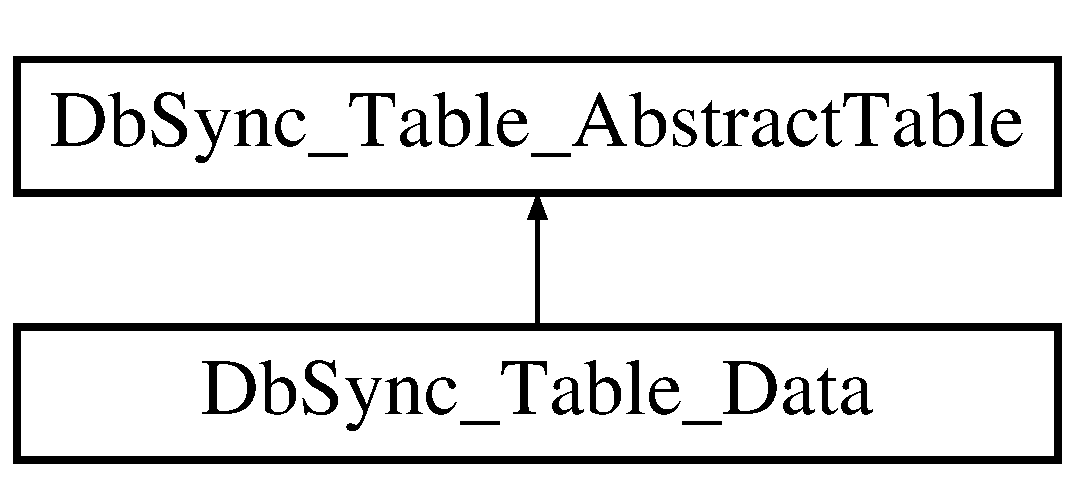
\includegraphics[height=2.000000cm]{classDbSync__Table__Data}
\end{center}
\end{figure}
\subsection*{Public Member Functions}
\begin{DoxyCompactItemize}
\item 
\hyperlink{classDbSync__Table__Data_a20a58562f3d88d85e5cb9b25f8f0e1dd}{getDataToStore} ()
\item 
\hyperlink{classDbSync__Table__Data_a9aabe67240f491f9b65371e5b94035c9}{push} (\$type=null)
\item 
\hyperlink{classDbSync__Table__Data_ac0e0899e75987cc0d69bff20cc373985}{isEmptyTable} ()
\end{DoxyCompactItemize}
\subsection*{Public Attributes}
\begin{DoxyCompactItemize}
\item 
\hypertarget{classDbSync__Table__Data_a8e2a613542f603afc3908ee00de3341c}{
const {\bfseries PUSH\_\-TYPE\_\-FORCE} = 1}
\label{classDbSync__Table__Data_a8e2a613542f603afc3908ee00de3341c}

\item 
\hypertarget{classDbSync__Table__Data_a8e7ab56799909572dfec44cb5f3cfa58}{
const {\bfseries PUSH\_\-TYPE\_\-MERGE} = 2}
\label{classDbSync__Table__Data_a8e7ab56799909572dfec44cb5f3cfa58}

\end{DoxyCompactItemize}
\subsection*{Protected Attributes}
\begin{DoxyCompactItemize}
\item 
\hypertarget{classDbSync__Table__Data_a7142c5a301b52c2e8ba51777314d1e15}{
{\bfseries \$\_\-filename} = 'data'}
\label{classDbSync__Table__Data_a7142c5a301b52c2e8ba51777314d1e15}

\end{DoxyCompactItemize}


\subsection{Member Function Documentation}
\hypertarget{classDbSync__Table__Data_a20a58562f3d88d85e5cb9b25f8f0e1dd}{
\index{DbSync\_\-Table\_\-Data@{DbSync\_\-Table\_\-Data}!getDataToStore@{getDataToStore}}
\index{getDataToStore@{getDataToStore}!DbSync_Table_Data@{DbSync\_\-Table\_\-Data}}
\subsubsection[{getDataToStore}]{\setlength{\rightskip}{0pt plus 5cm}DbSync\_\-Table\_\-Data::getDataToStore (
\begin{DoxyParamCaption}
{}
\end{DoxyParamCaption}
)}}
\label{classDbSync__Table__Data_a20a58562f3d88d85e5cb9b25f8f0e1dd}
Get data to store in config file

\begin{DoxyReturn}{Returns}
array 
\end{DoxyReturn}
\hypertarget{classDbSync__Table__Data_ac0e0899e75987cc0d69bff20cc373985}{
\index{DbSync\_\-Table\_\-Data@{DbSync\_\-Table\_\-Data}!isEmptyTable@{isEmptyTable}}
\index{isEmptyTable@{isEmptyTable}!DbSync_Table_Data@{DbSync\_\-Table\_\-Data}}
\subsubsection[{isEmptyTable}]{\setlength{\rightskip}{0pt plus 5cm}DbSync\_\-Table\_\-Data::isEmptyTable (
\begin{DoxyParamCaption}
{}
\end{DoxyParamCaption}
)}}
\label{classDbSync__Table__Data_ac0e0899e75987cc0d69bff20cc373985}
Is db table dirty

\begin{DoxyReturn}{Returns}
boolean 
\end{DoxyReturn}
\hypertarget{classDbSync__Table__Data_a9aabe67240f491f9b65371e5b94035c9}{
\index{DbSync\_\-Table\_\-Data@{DbSync\_\-Table\_\-Data}!push@{push}}
\index{push@{push}!DbSync_Table_Data@{DbSync\_\-Table\_\-Data}}
\subsubsection[{push}]{\setlength{\rightskip}{0pt plus 5cm}DbSync\_\-Table\_\-Data::push (
\begin{DoxyParamCaption}
\item[{\$}]{type = {\ttfamily null}}
\end{DoxyParamCaption}
)}}
\label{classDbSync__Table__Data_a9aabe67240f491f9b65371e5b94035c9}
Push data to db table


\begin{DoxyParams}[1]{Parameters}
boolen & {\em \$force} & false \\
\hline
boolen & {\em \$merge} & false \\
\hline
\end{DoxyParams}
\begin{DoxyReturn}{Returns}
boolen 
\end{DoxyReturn}

\begin{DoxyExceptions}{Exceptions}
{\em Exception} & \\
\hline
\end{DoxyExceptions}


The documentation for this class was generated from the following file:\begin{DoxyCompactItemize}
\item 
DbSync/Table/Data.php\end{DoxyCompactItemize}

\hypertarget{interfaceDbSync__Table__DbAdapter__AdapterInterface}{
\section{DbSync\_\-Table\_\-DbAdapter\_\-AdapterInterface Interface Reference}
\label{interfaceDbSync__Table__DbAdapter__AdapterInterface}\index{DbSync\_\-Table\_\-DbAdapter\_\-AdapterInterface@{DbSync\_\-Table\_\-DbAdapter\_\-AdapterInterface}}
}
Inheritance diagram for DbSync\_\-Table\_\-DbAdapter\_\-AdapterInterface:\begin{figure}[H]
\begin{center}
\leavevmode
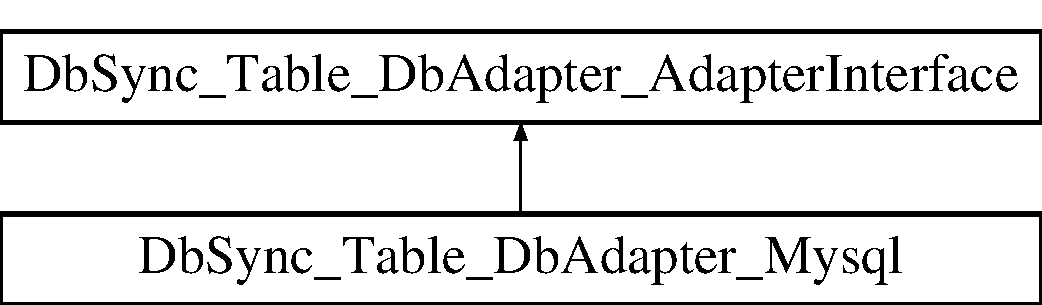
\includegraphics[height=2.000000cm]{interfaceDbSync__Table__DbAdapter__AdapterInterface}
\end{center}
\end{figure}
\subsection*{Public Member Functions}
\begin{DoxyCompactItemize}
\item 
\hyperlink{interfaceDbSync__Table__DbAdapter__AdapterInterface_acc52a558483c38b43d6c18de8d4af91c}{\_\-\_\-construct} (array \$config)
\item 
\hyperlink{interfaceDbSync__Table__DbAdapter__AdapterInterface_a44145e9ba3c9b176a846da4ec66b7709}{parseSchema} (\$tableName)
\item 
\hyperlink{interfaceDbSync__Table__DbAdapter__AdapterInterface_a5f0411aefd4e61b222c764523247089e}{createAlter} (\$config, \$tableName)
\item 
\hyperlink{interfaceDbSync__Table__DbAdapter__AdapterInterface_ac1a512f5f8995ab0cd14ebd8d6c8b4e5}{parseTrigger} (\$triggerName)
\item 
\hyperlink{interfaceDbSync__Table__DbAdapter__AdapterInterface_a9a5ea8d6bef1df0bfc0093e1ae513cde}{createTriggerSql} (\$config)
\item 
\hyperlink{interfaceDbSync__Table__DbAdapter__AdapterInterface_a201d09901524162b392e46774ed065c3}{execute} (\$sql)
\item 
\hyperlink{interfaceDbSync__Table__DbAdapter__AdapterInterface_aaea3134a13d12afd23e1fa1d44374736}{getTriggerList} ()
\item 
\hyperlink{interfaceDbSync__Table__DbAdapter__AdapterInterface_a2d71d9513cc7f87545f4185d89971191}{getTriggerInfo} (\$triggerName)
\item 
\hyperlink{interfaceDbSync__Table__DbAdapter__AdapterInterface_aa43cca3d069bbb2a1fe9f53310b50291}{getTableList} ()
\item 
\hyperlink{interfaceDbSync__Table__DbAdapter__AdapterInterface_ad407066eea549da5d8c7301476b75070}{hasTable} (\$tableName)
\item 
\hyperlink{interfaceDbSync__Table__DbAdapter__AdapterInterface_a93d8abfed28f5eaff4e4a0e9e944e018}{hasTrigger} (\$triggerName)
\item 
\hyperlink{interfaceDbSync__Table__DbAdapter__AdapterInterface_af67f030f94e4811d4ed55ef844ddda8e}{fetchData} (\$tableName)
\item 
\hyperlink{interfaceDbSync__Table__DbAdapter__AdapterInterface_a6f4051aa7dd67c963f0aaa37c96e319f}{insert} (\$data, \$tableName)
\item 
\hyperlink{interfaceDbSync__Table__DbAdapter__AdapterInterface_a7bfda16afa5d7a8400fe1c3de7dfb5c3}{merge} (\$data, \$tableName)
\item 
\hyperlink{interfaceDbSync__Table__DbAdapter__AdapterInterface_aa8df310d6667598487f35588d2c26ce4}{truncate} (\$tableName)
\item 
\hyperlink{interfaceDbSync__Table__DbAdapter__AdapterInterface_a8983e57eb3184fe7cf3107563a36ad82}{dropTable} (\$tableName)
\item 
\hyperlink{interfaceDbSync__Table__DbAdapter__AdapterInterface_a1a2d95ce258346ed1b1b2b08a70f0ae3}{dropTrigger} (\$triggerName)
\item 
\hyperlink{interfaceDbSync__Table__DbAdapter__AdapterInterface_ad93593e8305071020d6acce2f6ecbc5a}{isEmpty} (\$tableName)
\end{DoxyCompactItemize}


\subsection{Constructor \& Destructor Documentation}
\hypertarget{interfaceDbSync__Table__DbAdapter__AdapterInterface_acc52a558483c38b43d6c18de8d4af91c}{
\index{DbSync\_\-Table\_\-DbAdapter\_\-AdapterInterface@{DbSync\_\-Table\_\-DbAdapter\_\-AdapterInterface}!\_\-\_\-construct@{\_\-\_\-construct}}
\index{\_\-\_\-construct@{\_\-\_\-construct}!DbSync_Table_DbAdapter_AdapterInterface@{DbSync\_\-Table\_\-DbAdapter\_\-AdapterInterface}}
\subsubsection[{\_\-\_\-construct}]{\setlength{\rightskip}{0pt plus 5cm}DbSync\_\-Table\_\-DbAdapter\_\-AdapterInterface::\_\-\_\-construct (
\begin{DoxyParamCaption}
\item[{array \$}]{config}
\end{DoxyParamCaption}
)}}
\label{interfaceDbSync__Table__DbAdapter__AdapterInterface_acc52a558483c38b43d6c18de8d4af91c}
Constructor


\begin{DoxyParams}[1]{Parameters}
array & {\em \$config} & \\
\hline
\end{DoxyParams}


Implemented in \hyperlink{classDbSync__Table__DbAdapter__Mysql_a74e9a2b77c939b34d82f4b88bccc8151}{DbSync\_\-Table\_\-DbAdapter\_\-Mysql}.



\subsection{Member Function Documentation}
\hypertarget{interfaceDbSync__Table__DbAdapter__AdapterInterface_a5f0411aefd4e61b222c764523247089e}{
\index{DbSync\_\-Table\_\-DbAdapter\_\-AdapterInterface@{DbSync\_\-Table\_\-DbAdapter\_\-AdapterInterface}!createAlter@{createAlter}}
\index{createAlter@{createAlter}!DbSync_Table_DbAdapter_AdapterInterface@{DbSync\_\-Table\_\-DbAdapter\_\-AdapterInterface}}
\subsubsection[{createAlter}]{\setlength{\rightskip}{0pt plus 5cm}DbSync\_\-Table\_\-DbAdapter\_\-AdapterInterface::createAlter (
\begin{DoxyParamCaption}
\item[{\$}]{config, }
\item[{\$}]{tableName}
\end{DoxyParamCaption}
)}}
\label{interfaceDbSync__Table__DbAdapter__AdapterInterface_a5f0411aefd4e61b222c764523247089e}
Generate Alter Table


\begin{DoxyParams}[1]{Parameters}
array & {\em \$config} & \\
\hline
string & {\em \$tableName} & \\
\hline
\end{DoxyParams}
\begin{DoxyReturn}{Returns}
string 
\end{DoxyReturn}


Implemented in \hyperlink{classDbSync__Table__DbAdapter__Mysql_a02a1f1873924881f4a19cffbee049913}{DbSync\_\-Table\_\-DbAdapter\_\-Mysql}.

\hypertarget{interfaceDbSync__Table__DbAdapter__AdapterInterface_a9a5ea8d6bef1df0bfc0093e1ae513cde}{
\index{DbSync\_\-Table\_\-DbAdapter\_\-AdapterInterface@{DbSync\_\-Table\_\-DbAdapter\_\-AdapterInterface}!createTriggerSql@{createTriggerSql}}
\index{createTriggerSql@{createTriggerSql}!DbSync_Table_DbAdapter_AdapterInterface@{DbSync\_\-Table\_\-DbAdapter\_\-AdapterInterface}}
\subsubsection[{createTriggerSql}]{\setlength{\rightskip}{0pt plus 5cm}DbSync\_\-Table\_\-DbAdapter\_\-AdapterInterface::createTriggerSql (
\begin{DoxyParamCaption}
\item[{\$}]{config}
\end{DoxyParamCaption}
)}}
\label{interfaceDbSync__Table__DbAdapter__AdapterInterface_a9a5ea8d6bef1df0bfc0093e1ae513cde}
Generate trigger sql


\begin{DoxyParams}[1]{Parameters}
array & {\em \$config} & \\
\hline
\end{DoxyParams}
\begin{DoxyReturn}{Returns}
string 
\end{DoxyReturn}


Implemented in \hyperlink{classDbSync__Table__DbAdapter__Mysql_a4275474588eb1708c878b8381a9a9730}{DbSync\_\-Table\_\-DbAdapter\_\-Mysql}.

\hypertarget{interfaceDbSync__Table__DbAdapter__AdapterInterface_a8983e57eb3184fe7cf3107563a36ad82}{
\index{DbSync\_\-Table\_\-DbAdapter\_\-AdapterInterface@{DbSync\_\-Table\_\-DbAdapter\_\-AdapterInterface}!dropTable@{dropTable}}
\index{dropTable@{dropTable}!DbSync_Table_DbAdapter_AdapterInterface@{DbSync\_\-Table\_\-DbAdapter\_\-AdapterInterface}}
\subsubsection[{dropTable}]{\setlength{\rightskip}{0pt plus 5cm}DbSync\_\-Table\_\-DbAdapter\_\-AdapterInterface::dropTable (
\begin{DoxyParamCaption}
\item[{\$}]{tableName}
\end{DoxyParamCaption}
)}}
\label{interfaceDbSync__Table__DbAdapter__AdapterInterface_a8983e57eb3184fe7cf3107563a36ad82}
Drop table


\begin{DoxyParams}[1]{Parameters}
string & {\em \$tableName} & \\
\hline
\end{DoxyParams}
\begin{DoxyReturn}{Returns}
number 
\end{DoxyReturn}


Implemented in \hyperlink{classDbSync__Table__DbAdapter__Mysql_ae489c716f124c842b3effd83433b0bda}{DbSync\_\-Table\_\-DbAdapter\_\-Mysql}.

\hypertarget{interfaceDbSync__Table__DbAdapter__AdapterInterface_a1a2d95ce258346ed1b1b2b08a70f0ae3}{
\index{DbSync\_\-Table\_\-DbAdapter\_\-AdapterInterface@{DbSync\_\-Table\_\-DbAdapter\_\-AdapterInterface}!dropTrigger@{dropTrigger}}
\index{dropTrigger@{dropTrigger}!DbSync_Table_DbAdapter_AdapterInterface@{DbSync\_\-Table\_\-DbAdapter\_\-AdapterInterface}}
\subsubsection[{dropTrigger}]{\setlength{\rightskip}{0pt plus 5cm}DbSync\_\-Table\_\-DbAdapter\_\-AdapterInterface::dropTrigger (
\begin{DoxyParamCaption}
\item[{\$}]{triggerName}
\end{DoxyParamCaption}
)}}
\label{interfaceDbSync__Table__DbAdapter__AdapterInterface_a1a2d95ce258346ed1b1b2b08a70f0ae3}
Drop trigger


\begin{DoxyParams}[1]{Parameters}
string & {\em \$triggerName} & \\
\hline
\end{DoxyParams}
\begin{DoxyReturn}{Returns}
number 
\end{DoxyReturn}


Implemented in \hyperlink{classDbSync__Table__DbAdapter__Mysql_a47230a67ff7e8c926ee6fb421764e5ec}{DbSync\_\-Table\_\-DbAdapter\_\-Mysql}.

\hypertarget{interfaceDbSync__Table__DbAdapter__AdapterInterface_a201d09901524162b392e46774ed065c3}{
\index{DbSync\_\-Table\_\-DbAdapter\_\-AdapterInterface@{DbSync\_\-Table\_\-DbAdapter\_\-AdapterInterface}!execute@{execute}}
\index{execute@{execute}!DbSync_Table_DbAdapter_AdapterInterface@{DbSync\_\-Table\_\-DbAdapter\_\-AdapterInterface}}
\subsubsection[{execute}]{\setlength{\rightskip}{0pt plus 5cm}DbSync\_\-Table\_\-DbAdapter\_\-AdapterInterface::execute (
\begin{DoxyParamCaption}
\item[{\$}]{sql}
\end{DoxyParamCaption}
)}}
\label{interfaceDbSync__Table__DbAdapter__AdapterInterface_a201d09901524162b392e46774ed065c3}
Execute sql query


\begin{DoxyParams}[1]{Parameters}
string & {\em \$sql} & \\
\hline
\end{DoxyParams}
\begin{DoxyReturn}{Returns}
integer 
\end{DoxyReturn}


Implemented in \hyperlink{classDbSync__Table__DbAdapter__Mysql_a9c0b01e49c27d2cabcb5c9245b8f6ad7}{DbSync\_\-Table\_\-DbAdapter\_\-Mysql}.

\hypertarget{interfaceDbSync__Table__DbAdapter__AdapterInterface_af67f030f94e4811d4ed55ef844ddda8e}{
\index{DbSync\_\-Table\_\-DbAdapter\_\-AdapterInterface@{DbSync\_\-Table\_\-DbAdapter\_\-AdapterInterface}!fetchData@{fetchData}}
\index{fetchData@{fetchData}!DbSync_Table_DbAdapter_AdapterInterface@{DbSync\_\-Table\_\-DbAdapter\_\-AdapterInterface}}
\subsubsection[{fetchData}]{\setlength{\rightskip}{0pt plus 5cm}DbSync\_\-Table\_\-DbAdapter\_\-AdapterInterface::fetchData (
\begin{DoxyParamCaption}
\item[{\$}]{tableName}
\end{DoxyParamCaption}
)}}
\label{interfaceDbSync__Table__DbAdapter__AdapterInterface_af67f030f94e4811d4ed55ef844ddda8e}
Fetch all data from table

\begin{DoxyReturn}{Returns}
array 
\end{DoxyReturn}


Implemented in \hyperlink{classDbSync__Table__DbAdapter__Mysql_acefde6ec7836aa5a0106bca42501c37c}{DbSync\_\-Table\_\-DbAdapter\_\-Mysql}.

\hypertarget{interfaceDbSync__Table__DbAdapter__AdapterInterface_aa43cca3d069bbb2a1fe9f53310b50291}{
\index{DbSync\_\-Table\_\-DbAdapter\_\-AdapterInterface@{DbSync\_\-Table\_\-DbAdapter\_\-AdapterInterface}!getTableList@{getTableList}}
\index{getTableList@{getTableList}!DbSync_Table_DbAdapter_AdapterInterface@{DbSync\_\-Table\_\-DbAdapter\_\-AdapterInterface}}
\subsubsection[{getTableList}]{\setlength{\rightskip}{0pt plus 5cm}DbSync\_\-Table\_\-DbAdapter\_\-AdapterInterface::getTableList (
\begin{DoxyParamCaption}
{}
\end{DoxyParamCaption}
)}}
\label{interfaceDbSync__Table__DbAdapter__AdapterInterface_aa43cca3d069bbb2a1fe9f53310b50291}
Get tables list

\begin{DoxyReturn}{Returns}
array 
\end{DoxyReturn}


Implemented in \hyperlink{classDbSync__Table__DbAdapter__Mysql_a91839f71bb8ed628f3e18ce1d8b330ba}{DbSync\_\-Table\_\-DbAdapter\_\-Mysql}.

\hypertarget{interfaceDbSync__Table__DbAdapter__AdapterInterface_a2d71d9513cc7f87545f4185d89971191}{
\index{DbSync\_\-Table\_\-DbAdapter\_\-AdapterInterface@{DbSync\_\-Table\_\-DbAdapter\_\-AdapterInterface}!getTriggerInfo@{getTriggerInfo}}
\index{getTriggerInfo@{getTriggerInfo}!DbSync_Table_DbAdapter_AdapterInterface@{DbSync\_\-Table\_\-DbAdapter\_\-AdapterInterface}}
\subsubsection[{getTriggerInfo}]{\setlength{\rightskip}{0pt plus 5cm}DbSync\_\-Table\_\-DbAdapter\_\-AdapterInterface::getTriggerInfo (
\begin{DoxyParamCaption}
\item[{\$}]{triggerName}
\end{DoxyParamCaption}
)}}
\label{interfaceDbSync__Table__DbAdapter__AdapterInterface_a2d71d9513cc7f87545f4185d89971191}
Get trigger info

\begin{DoxyReturn}{Returns}
string 
\end{DoxyReturn}


Implemented in \hyperlink{classDbSync__Table__DbAdapter__Mysql_ae48113aa663f1fc9b1fda9d52c55fdb5}{DbSync\_\-Table\_\-DbAdapter\_\-Mysql}.

\hypertarget{interfaceDbSync__Table__DbAdapter__AdapterInterface_aaea3134a13d12afd23e1fa1d44374736}{
\index{DbSync\_\-Table\_\-DbAdapter\_\-AdapterInterface@{DbSync\_\-Table\_\-DbAdapter\_\-AdapterInterface}!getTriggerList@{getTriggerList}}
\index{getTriggerList@{getTriggerList}!DbSync_Table_DbAdapter_AdapterInterface@{DbSync\_\-Table\_\-DbAdapter\_\-AdapterInterface}}
\subsubsection[{getTriggerList}]{\setlength{\rightskip}{0pt plus 5cm}DbSync\_\-Table\_\-DbAdapter\_\-AdapterInterface::getTriggerList (
\begin{DoxyParamCaption}
{}
\end{DoxyParamCaption}
)}}
\label{interfaceDbSync__Table__DbAdapter__AdapterInterface_aaea3134a13d12afd23e1fa1d44374736}
Get triggers list

\begin{DoxyReturn}{Returns}
array 
\end{DoxyReturn}
\hypertarget{interfaceDbSync__Table__DbAdapter__AdapterInterface_ad407066eea549da5d8c7301476b75070}{
\index{DbSync\_\-Table\_\-DbAdapter\_\-AdapterInterface@{DbSync\_\-Table\_\-DbAdapter\_\-AdapterInterface}!hasTable@{hasTable}}
\index{hasTable@{hasTable}!DbSync_Table_DbAdapter_AdapterInterface@{DbSync\_\-Table\_\-DbAdapter\_\-AdapterInterface}}
\subsubsection[{hasTable}]{\setlength{\rightskip}{0pt plus 5cm}DbSync\_\-Table\_\-DbAdapter\_\-AdapterInterface::hasTable (
\begin{DoxyParamCaption}
\item[{\$}]{tableName}
\end{DoxyParamCaption}
)}}
\label{interfaceDbSync__Table__DbAdapter__AdapterInterface_ad407066eea549da5d8c7301476b75070}
Is db table exists

\begin{DoxyReturn}{Returns}
boolen 
\end{DoxyReturn}


Implemented in \hyperlink{classDbSync__Table__DbAdapter__Mysql_a79a6ba5c7d73794dfd4e141471ff9e19}{DbSync\_\-Table\_\-DbAdapter\_\-Mysql}.

\hypertarget{interfaceDbSync__Table__DbAdapter__AdapterInterface_a93d8abfed28f5eaff4e4a0e9e944e018}{
\index{DbSync\_\-Table\_\-DbAdapter\_\-AdapterInterface@{DbSync\_\-Table\_\-DbAdapter\_\-AdapterInterface}!hasTrigger@{hasTrigger}}
\index{hasTrigger@{hasTrigger}!DbSync_Table_DbAdapter_AdapterInterface@{DbSync\_\-Table\_\-DbAdapter\_\-AdapterInterface}}
\subsubsection[{hasTrigger}]{\setlength{\rightskip}{0pt plus 5cm}DbSync\_\-Table\_\-DbAdapter\_\-AdapterInterface::hasTrigger (
\begin{DoxyParamCaption}
\item[{\$}]{triggerName}
\end{DoxyParamCaption}
)}}
\label{interfaceDbSync__Table__DbAdapter__AdapterInterface_a93d8abfed28f5eaff4e4a0e9e944e018}
Is db trigger exists

\begin{DoxyReturn}{Returns}
boolen 
\end{DoxyReturn}


Implemented in \hyperlink{classDbSync__Table__DbAdapter__Mysql_a3099dfb064dcf136150cff82d36ded91}{DbSync\_\-Table\_\-DbAdapter\_\-Mysql}.

\hypertarget{interfaceDbSync__Table__DbAdapter__AdapterInterface_a6f4051aa7dd67c963f0aaa37c96e319f}{
\index{DbSync\_\-Table\_\-DbAdapter\_\-AdapterInterface@{DbSync\_\-Table\_\-DbAdapter\_\-AdapterInterface}!insert@{insert}}
\index{insert@{insert}!DbSync_Table_DbAdapter_AdapterInterface@{DbSync\_\-Table\_\-DbAdapter\_\-AdapterInterface}}
\subsubsection[{insert}]{\setlength{\rightskip}{0pt plus 5cm}DbSync\_\-Table\_\-DbAdapter\_\-AdapterInterface::insert (
\begin{DoxyParamCaption}
\item[{\$}]{data, }
\item[{\$}]{tableName}
\end{DoxyParamCaption}
)}}
\label{interfaceDbSync__Table__DbAdapter__AdapterInterface_a6f4051aa7dd67c963f0aaa37c96e319f}
Push data to db table


\begin{DoxyParams}[1]{Parameters}
boolen & {\em \$force} & \\
\hline
\end{DoxyParams}
\begin{DoxyReturn}{Returns}
boolen 
\end{DoxyReturn}

\begin{DoxyExceptions}{Exceptions}
{\em Exception} & \\
\hline
\end{DoxyExceptions}


Implemented in \hyperlink{classDbSync__Table__DbAdapter__Mysql_a2f35fe8a01719833f9f0bdeb284e7620}{DbSync\_\-Table\_\-DbAdapter\_\-Mysql}.

\hypertarget{interfaceDbSync__Table__DbAdapter__AdapterInterface_ad93593e8305071020d6acce2f6ecbc5a}{
\index{DbSync\_\-Table\_\-DbAdapter\_\-AdapterInterface@{DbSync\_\-Table\_\-DbAdapter\_\-AdapterInterface}!isEmpty@{isEmpty}}
\index{isEmpty@{isEmpty}!DbSync_Table_DbAdapter_AdapterInterface@{DbSync\_\-Table\_\-DbAdapter\_\-AdapterInterface}}
\subsubsection[{isEmpty}]{\setlength{\rightskip}{0pt plus 5cm}DbSync\_\-Table\_\-DbAdapter\_\-AdapterInterface::isEmpty (
\begin{DoxyParamCaption}
\item[{\$}]{tableName}
\end{DoxyParamCaption}
)}}
\label{interfaceDbSync__Table__DbAdapter__AdapterInterface_ad93593e8305071020d6acce2f6ecbc5a}
Is db table empty


\begin{DoxyParams}[1]{Parameters}
string & {\em \$tableName} & \\
\hline
\end{DoxyParams}
\begin{DoxyReturn}{Returns}
boolean 
\end{DoxyReturn}


Implemented in \hyperlink{classDbSync__Table__DbAdapter__Mysql_a492a22c32d988393ab5456eec80b6923}{DbSync\_\-Table\_\-DbAdapter\_\-Mysql}.

\hypertarget{interfaceDbSync__Table__DbAdapter__AdapterInterface_a7bfda16afa5d7a8400fe1c3de7dfb5c3}{
\index{DbSync\_\-Table\_\-DbAdapter\_\-AdapterInterface@{DbSync\_\-Table\_\-DbAdapter\_\-AdapterInterface}!merge@{merge}}
\index{merge@{merge}!DbSync_Table_DbAdapter_AdapterInterface@{DbSync\_\-Table\_\-DbAdapter\_\-AdapterInterface}}
\subsubsection[{merge}]{\setlength{\rightskip}{0pt plus 5cm}DbSync\_\-Table\_\-DbAdapter\_\-AdapterInterface::merge (
\begin{DoxyParamCaption}
\item[{\$}]{data, }
\item[{\$}]{tableName}
\end{DoxyParamCaption}
)}}
\label{interfaceDbSync__Table__DbAdapter__AdapterInterface_a7bfda16afa5d7a8400fe1c3de7dfb5c3}
Merge data to db table


\begin{DoxyExceptions}{Exceptions}
{\em Exception} & \\
\hline
\end{DoxyExceptions}
\begin{DoxyReturn}{Returns}
boolean 
\end{DoxyReturn}


Implemented in \hyperlink{classDbSync__Table__DbAdapter__Mysql_a15ec3683b5473be0e2c7a24b9e78dfb5}{DbSync\_\-Table\_\-DbAdapter\_\-Mysql}.

\hypertarget{interfaceDbSync__Table__DbAdapter__AdapterInterface_a44145e9ba3c9b176a846da4ec66b7709}{
\index{DbSync\_\-Table\_\-DbAdapter\_\-AdapterInterface@{DbSync\_\-Table\_\-DbAdapter\_\-AdapterInterface}!parseSchema@{parseSchema}}
\index{parseSchema@{parseSchema}!DbSync_Table_DbAdapter_AdapterInterface@{DbSync\_\-Table\_\-DbAdapter\_\-AdapterInterface}}
\subsubsection[{parseSchema}]{\setlength{\rightskip}{0pt plus 5cm}DbSync\_\-Table\_\-DbAdapter\_\-AdapterInterface::parseSchema (
\begin{DoxyParamCaption}
\item[{\$}]{tableName}
\end{DoxyParamCaption}
)}}
\label{interfaceDbSync__Table__DbAdapter__AdapterInterface_a44145e9ba3c9b176a846da4ec66b7709}
Parse schema

\begin{DoxyReturn}{Returns}
array 
\end{DoxyReturn}


Implemented in \hyperlink{classDbSync__Table__DbAdapter__Mysql_af7b83b6b5d51bb77814d52cec3cce5af}{DbSync\_\-Table\_\-DbAdapter\_\-Mysql}.

\hypertarget{interfaceDbSync__Table__DbAdapter__AdapterInterface_ac1a512f5f8995ab0cd14ebd8d6c8b4e5}{
\index{DbSync\_\-Table\_\-DbAdapter\_\-AdapterInterface@{DbSync\_\-Table\_\-DbAdapter\_\-AdapterInterface}!parseTrigger@{parseTrigger}}
\index{parseTrigger@{parseTrigger}!DbSync_Table_DbAdapter_AdapterInterface@{DbSync\_\-Table\_\-DbAdapter\_\-AdapterInterface}}
\subsubsection[{parseTrigger}]{\setlength{\rightskip}{0pt plus 5cm}DbSync\_\-Table\_\-DbAdapter\_\-AdapterInterface::parseTrigger (
\begin{DoxyParamCaption}
\item[{\$}]{triggerName}
\end{DoxyParamCaption}
)}}
\label{interfaceDbSync__Table__DbAdapter__AdapterInterface_ac1a512f5f8995ab0cd14ebd8d6c8b4e5}
Fetch db triggers

\begin{DoxyReturn}{Returns}
string 
\end{DoxyReturn}


Implemented in \hyperlink{classDbSync__Table__DbAdapter__Mysql_a0b16aae79092f4039b42d2deec54b071}{DbSync\_\-Table\_\-DbAdapter\_\-Mysql}.

\hypertarget{interfaceDbSync__Table__DbAdapter__AdapterInterface_aa8df310d6667598487f35588d2c26ce4}{
\index{DbSync\_\-Table\_\-DbAdapter\_\-AdapterInterface@{DbSync\_\-Table\_\-DbAdapter\_\-AdapterInterface}!truncate@{truncate}}
\index{truncate@{truncate}!DbSync_Table_DbAdapter_AdapterInterface@{DbSync\_\-Table\_\-DbAdapter\_\-AdapterInterface}}
\subsubsection[{truncate}]{\setlength{\rightskip}{0pt plus 5cm}DbSync\_\-Table\_\-DbAdapter\_\-AdapterInterface::truncate (
\begin{DoxyParamCaption}
\item[{\$}]{tableName}
\end{DoxyParamCaption}
)}}
\label{interfaceDbSync__Table__DbAdapter__AdapterInterface_aa8df310d6667598487f35588d2c26ce4}
Truncate table


\begin{DoxyParams}[1]{Parameters}
string & {\em \$tableName} & \\
\hline
\end{DoxyParams}
\begin{DoxyReturn}{Returns}
number 
\end{DoxyReturn}


Implemented in \hyperlink{classDbSync__Table__DbAdapter__Mysql_a3bd21ebc1da5c9eb8b17c884201226d8}{DbSync\_\-Table\_\-DbAdapter\_\-Mysql}.



The documentation for this interface was generated from the following file:\begin{DoxyCompactItemize}
\item 
DbSync/Table/DbAdapter/AdapterInterface.php\end{DoxyCompactItemize}

\hypertarget{classDbSync__Table__DbAdapter__Mysql}{
\section{DbSync\_\-Table\_\-DbAdapter\_\-Mysql Class Reference}
\label{classDbSync__Table__DbAdapter__Mysql}\index{DbSync\_\-Table\_\-DbAdapter\_\-Mysql@{DbSync\_\-Table\_\-DbAdapter\_\-Mysql}}
}
Inheritance diagram for DbSync\_\-Table\_\-DbAdapter\_\-Mysql:\begin{figure}[H]
\begin{center}
\leavevmode
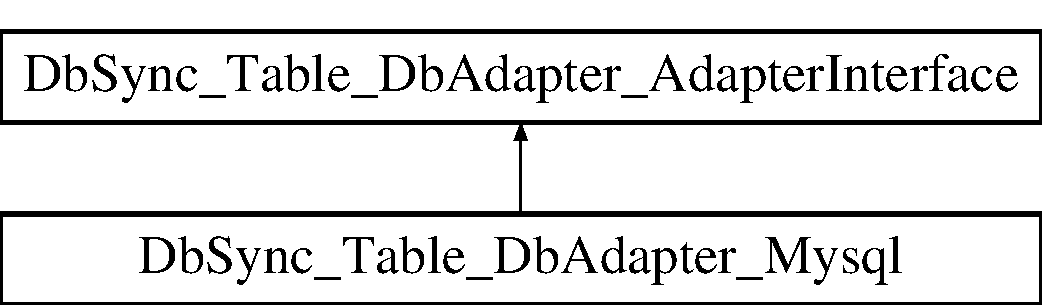
\includegraphics[height=2.000000cm]{classDbSync__Table__DbAdapter__Mysql}
\end{center}
\end{figure}
\subsection*{Public Member Functions}
\begin{DoxyCompactItemize}
\item 
\hyperlink{classDbSync__Table__DbAdapter__Mysql_a74e9a2b77c939b34d82f4b88bccc8151}{\_\-\_\-construct} (array \$config)
\item 
\hyperlink{classDbSync__Table__DbAdapter__Mysql_a3c000f13b6eac670c0dd9c85de31ac49}{getConnection} ()
\item 
\hyperlink{classDbSync__Table__DbAdapter__Mysql_a644d3a69901a0565a480721e652d5fec}{setConnection} (PDO \$connection)
\item 
\hyperlink{classDbSync__Table__DbAdapter__Mysql_af7b83b6b5d51bb77814d52cec3cce5af}{parseSchema} (\$tableName)
\item 
\hyperlink{classDbSync__Table__DbAdapter__Mysql_a02a1f1873924881f4a19cffbee049913}{createAlter} (\$config, \$tableName)
\item 
\hyperlink{classDbSync__Table__DbAdapter__Mysql_a0b16aae79092f4039b42d2deec54b071}{parseTrigger} (\$triggerName)
\item 
\hyperlink{classDbSync__Table__DbAdapter__Mysql_a4275474588eb1708c878b8381a9a9730}{createTriggerSql} (\$config)
\item 
\hyperlink{classDbSync__Table__DbAdapter__Mysql_a9c0b01e49c27d2cabcb5c9245b8f6ad7}{execute} (\$sql)
\item 
\hyperlink{classDbSync__Table__DbAdapter__Mysql_a8a0a871cc633ac6ed3c6cfbac2ea9f01}{getTriggerList} (\$tables=array())
\item 
\hyperlink{classDbSync__Table__DbAdapter__Mysql_ae48113aa663f1fc9b1fda9d52c55fdb5}{getTriggerInfo} (\$triggerName)
\item 
\hyperlink{classDbSync__Table__DbAdapter__Mysql_a91839f71bb8ed628f3e18ce1d8b330ba}{getTableList} ()
\item 
\hyperlink{classDbSync__Table__DbAdapter__Mysql_a79a6ba5c7d73794dfd4e141471ff9e19}{hasTable} (\$tableName)
\item 
\hyperlink{classDbSync__Table__DbAdapter__Mysql_a3099dfb064dcf136150cff82d36ded91}{hasTrigger} (\$triggerName)
\item 
\hyperlink{classDbSync__Table__DbAdapter__Mysql_acefde6ec7836aa5a0106bca42501c37c}{fetchData} (\$tableName)
\item 
\hyperlink{classDbSync__Table__DbAdapter__Mysql_a2f35fe8a01719833f9f0bdeb284e7620}{insert} (\$data, \$tableName)
\item 
\hyperlink{classDbSync__Table__DbAdapter__Mysql_a15ec3683b5473be0e2c7a24b9e78dfb5}{merge} (\$data, \$tableName)
\item 
\hyperlink{classDbSync__Table__DbAdapter__Mysql_a3bd21ebc1da5c9eb8b17c884201226d8}{truncate} (\$tableName)
\item 
\hyperlink{classDbSync__Table__DbAdapter__Mysql_ae489c716f124c842b3effd83433b0bda}{dropTable} (\$tableName)
\item 
\hyperlink{classDbSync__Table__DbAdapter__Mysql_a47230a67ff7e8c926ee6fb421764e5ec}{dropTrigger} (\$triggerName)
\item 
\hyperlink{classDbSync__Table__DbAdapter__Mysql_a492a22c32d988393ab5456eec80b6923}{isEmpty} (\$tableName)
\end{DoxyCompactItemize}
\subsection*{Protected Member Functions}
\begin{DoxyCompactItemize}
\item 
\hyperlink{classDbSync__Table__DbAdapter__Mysql_a56894feff172b0d77cad42b4aebf0ade}{\_\-hasPrimaryKey} (\$tableName)
\item 
\hyperlink{classDbSync__Table__DbAdapter__Mysql_acc41d16b369c99409607267268e0764e}{\_\-getIndexes} (\$tableName)
\item 
\hyperlink{classDbSync__Table__DbAdapter__Mysql_a1a7d3bca83371bcb16cd7a59f810bb58}{\_\-getColumnSql} (\$name, \$config, \$after=null)
\end{DoxyCompactItemize}
\subsection*{Protected Attributes}
\begin{DoxyCompactItemize}
\item 
\hypertarget{classDbSync__Table__DbAdapter__Mysql_ae64f6e1da0331b741a73251aa5bec165}{
{\bfseries \$\_\-db}}
\label{classDbSync__Table__DbAdapter__Mysql_ae64f6e1da0331b741a73251aa5bec165}

\end{DoxyCompactItemize}


\subsection{Constructor \& Destructor Documentation}
\hypertarget{classDbSync__Table__DbAdapter__Mysql_a74e9a2b77c939b34d82f4b88bccc8151}{
\index{DbSync\_\-Table\_\-DbAdapter\_\-Mysql@{DbSync\_\-Table\_\-DbAdapter\_\-Mysql}!\_\-\_\-construct@{\_\-\_\-construct}}
\index{\_\-\_\-construct@{\_\-\_\-construct}!DbSync_Table_DbAdapter_Mysql@{DbSync\_\-Table\_\-DbAdapter\_\-Mysql}}
\subsubsection[{\_\-\_\-construct}]{\setlength{\rightskip}{0pt plus 5cm}DbSync\_\-Table\_\-DbAdapter\_\-Mysql::\_\-\_\-construct (
\begin{DoxyParamCaption}
\item[{array \$}]{config}
\end{DoxyParamCaption}
)}}
\label{classDbSync__Table__DbAdapter__Mysql_a74e9a2b77c939b34d82f4b88bccc8151}
Constructor


\begin{DoxyParams}[1]{Parameters}
array & {\em \$config} & \\
\hline
\end{DoxyParams}


Implements \hyperlink{interfaceDbSync__Table__DbAdapter__AdapterInterface_acc52a558483c38b43d6c18de8d4af91c}{DbSync\_\-Table\_\-DbAdapter\_\-AdapterInterface}.



\subsection{Member Function Documentation}
\hypertarget{classDbSync__Table__DbAdapter__Mysql_a1a7d3bca83371bcb16cd7a59f810bb58}{
\index{DbSync\_\-Table\_\-DbAdapter\_\-Mysql@{DbSync\_\-Table\_\-DbAdapter\_\-Mysql}!\_\-getColumnSql@{\_\-getColumnSql}}
\index{\_\-getColumnSql@{\_\-getColumnSql}!DbSync_Table_DbAdapter_Mysql@{DbSync\_\-Table\_\-DbAdapter\_\-Mysql}}
\subsubsection[{\_\-getColumnSql}]{\setlength{\rightskip}{0pt plus 5cm}DbSync\_\-Table\_\-DbAdapter\_\-Mysql::\_\-getColumnSql (
\begin{DoxyParamCaption}
\item[{\$}]{name, }
\item[{\$}]{config, }
\item[{\$}]{after = {\ttfamily null}}
\end{DoxyParamCaption}
)\hspace{0.3cm}{\ttfamily  \mbox{[}protected\mbox{]}}}}
\label{classDbSync__Table__DbAdapter__Mysql_a1a7d3bca83371bcb16cd7a59f810bb58}
Get column sql


\begin{DoxyParams}[1]{Parameters}
string & {\em \$name} & \\
\hline
array & {\em \$config} & \\
\hline
string & {\em \$after} & \\
\hline
\end{DoxyParams}
\begin{DoxyReturn}{Returns}
string 
\end{DoxyReturn}
\hypertarget{classDbSync__Table__DbAdapter__Mysql_acc41d16b369c99409607267268e0764e}{
\index{DbSync\_\-Table\_\-DbAdapter\_\-Mysql@{DbSync\_\-Table\_\-DbAdapter\_\-Mysql}!\_\-getIndexes@{\_\-getIndexes}}
\index{\_\-getIndexes@{\_\-getIndexes}!DbSync_Table_DbAdapter_Mysql@{DbSync\_\-Table\_\-DbAdapter\_\-Mysql}}
\subsubsection[{\_\-getIndexes}]{\setlength{\rightskip}{0pt plus 5cm}DbSync\_\-Table\_\-DbAdapter\_\-Mysql::\_\-getIndexes (
\begin{DoxyParamCaption}
\item[{\$}]{tableName}
\end{DoxyParamCaption}
)\hspace{0.3cm}{\ttfamily  \mbox{[}protected\mbox{]}}}}
\label{classDbSync__Table__DbAdapter__Mysql_acc41d16b369c99409607267268e0764e}
Get table indexes


\begin{DoxyParams}[1]{Parameters}
string & {\em \$tableName} & \\
\hline
\end{DoxyParams}
\begin{DoxyReturn}{Returns}
array 
\end{DoxyReturn}
\hypertarget{classDbSync__Table__DbAdapter__Mysql_a56894feff172b0d77cad42b4aebf0ade}{
\index{DbSync\_\-Table\_\-DbAdapter\_\-Mysql@{DbSync\_\-Table\_\-DbAdapter\_\-Mysql}!\_\-hasPrimaryKey@{\_\-hasPrimaryKey}}
\index{\_\-hasPrimaryKey@{\_\-hasPrimaryKey}!DbSync_Table_DbAdapter_Mysql@{DbSync\_\-Table\_\-DbAdapter\_\-Mysql}}
\subsubsection[{\_\-hasPrimaryKey}]{\setlength{\rightskip}{0pt plus 5cm}DbSync\_\-Table\_\-DbAdapter\_\-Mysql::\_\-hasPrimaryKey (
\begin{DoxyParamCaption}
\item[{\$}]{tableName}
\end{DoxyParamCaption}
)\hspace{0.3cm}{\ttfamily  \mbox{[}protected\mbox{]}}}}
\label{classDbSync__Table__DbAdapter__Mysql_a56894feff172b0d77cad42b4aebf0ade}
Has table a primary key


\begin{DoxyParams}[1]{Parameters}
string & {\em \$tableName} & \\
\hline
\end{DoxyParams}
\begin{DoxyReturn}{Returns}
boolen 
\end{DoxyReturn}
\hypertarget{classDbSync__Table__DbAdapter__Mysql_a02a1f1873924881f4a19cffbee049913}{
\index{DbSync\_\-Table\_\-DbAdapter\_\-Mysql@{DbSync\_\-Table\_\-DbAdapter\_\-Mysql}!createAlter@{createAlter}}
\index{createAlter@{createAlter}!DbSync_Table_DbAdapter_Mysql@{DbSync\_\-Table\_\-DbAdapter\_\-Mysql}}
\subsubsection[{createAlter}]{\setlength{\rightskip}{0pt plus 5cm}DbSync\_\-Table\_\-DbAdapter\_\-Mysql::createAlter (
\begin{DoxyParamCaption}
\item[{\$}]{config, }
\item[{\$}]{tableName}
\end{DoxyParamCaption}
)}}
\label{classDbSync__Table__DbAdapter__Mysql_a02a1f1873924881f4a19cffbee049913}
Generate Alter Table


\begin{DoxyParams}[1]{Parameters}
array & {\em \$config} & \\
\hline
string & {\em \$tableName} & \\
\hline
\end{DoxyParams}
\begin{DoxyReturn}{Returns}
string 
\end{DoxyReturn}


Implements \hyperlink{interfaceDbSync__Table__DbAdapter__AdapterInterface_a5f0411aefd4e61b222c764523247089e}{DbSync\_\-Table\_\-DbAdapter\_\-AdapterInterface}.

\hypertarget{classDbSync__Table__DbAdapter__Mysql_a4275474588eb1708c878b8381a9a9730}{
\index{DbSync\_\-Table\_\-DbAdapter\_\-Mysql@{DbSync\_\-Table\_\-DbAdapter\_\-Mysql}!createTriggerSql@{createTriggerSql}}
\index{createTriggerSql@{createTriggerSql}!DbSync_Table_DbAdapter_Mysql@{DbSync\_\-Table\_\-DbAdapter\_\-Mysql}}
\subsubsection[{createTriggerSql}]{\setlength{\rightskip}{0pt plus 5cm}DbSync\_\-Table\_\-DbAdapter\_\-Mysql::createTriggerSql (
\begin{DoxyParamCaption}
\item[{\$}]{config}
\end{DoxyParamCaption}
)}}
\label{classDbSync__Table__DbAdapter__Mysql_a4275474588eb1708c878b8381a9a9730}
Generate trigger sql


\begin{DoxyParams}[1]{Parameters}
array & {\em \$config} & \\
\hline
\end{DoxyParams}
\begin{DoxyReturn}{Returns}
string 
\end{DoxyReturn}


Implements \hyperlink{interfaceDbSync__Table__DbAdapter__AdapterInterface_a9a5ea8d6bef1df0bfc0093e1ae513cde}{DbSync\_\-Table\_\-DbAdapter\_\-AdapterInterface}.

\hypertarget{classDbSync__Table__DbAdapter__Mysql_ae489c716f124c842b3effd83433b0bda}{
\index{DbSync\_\-Table\_\-DbAdapter\_\-Mysql@{DbSync\_\-Table\_\-DbAdapter\_\-Mysql}!dropTable@{dropTable}}
\index{dropTable@{dropTable}!DbSync_Table_DbAdapter_Mysql@{DbSync\_\-Table\_\-DbAdapter\_\-Mysql}}
\subsubsection[{dropTable}]{\setlength{\rightskip}{0pt plus 5cm}DbSync\_\-Table\_\-DbAdapter\_\-Mysql::dropTable (
\begin{DoxyParamCaption}
\item[{\$}]{tableName}
\end{DoxyParamCaption}
)}}
\label{classDbSync__Table__DbAdapter__Mysql_ae489c716f124c842b3effd83433b0bda}
Drop table


\begin{DoxyParams}[1]{Parameters}
string & {\em \$tableName} & \\
\hline
\end{DoxyParams}
\begin{DoxyReturn}{Returns}
number 
\end{DoxyReturn}


Implements \hyperlink{interfaceDbSync__Table__DbAdapter__AdapterInterface_a8983e57eb3184fe7cf3107563a36ad82}{DbSync\_\-Table\_\-DbAdapter\_\-AdapterInterface}.

\hypertarget{classDbSync__Table__DbAdapter__Mysql_a47230a67ff7e8c926ee6fb421764e5ec}{
\index{DbSync\_\-Table\_\-DbAdapter\_\-Mysql@{DbSync\_\-Table\_\-DbAdapter\_\-Mysql}!dropTrigger@{dropTrigger}}
\index{dropTrigger@{dropTrigger}!DbSync_Table_DbAdapter_Mysql@{DbSync\_\-Table\_\-DbAdapter\_\-Mysql}}
\subsubsection[{dropTrigger}]{\setlength{\rightskip}{0pt plus 5cm}DbSync\_\-Table\_\-DbAdapter\_\-Mysql::dropTrigger (
\begin{DoxyParamCaption}
\item[{\$}]{triggerName}
\end{DoxyParamCaption}
)}}
\label{classDbSync__Table__DbAdapter__Mysql_a47230a67ff7e8c926ee6fb421764e5ec}
Drop trigger


\begin{DoxyParams}[1]{Parameters}
string & {\em \$triggerName} & \\
\hline
\end{DoxyParams}
\begin{DoxyReturn}{Returns}
number 
\end{DoxyReturn}


Implements \hyperlink{interfaceDbSync__Table__DbAdapter__AdapterInterface_a1a2d95ce258346ed1b1b2b08a70f0ae3}{DbSync\_\-Table\_\-DbAdapter\_\-AdapterInterface}.

\hypertarget{classDbSync__Table__DbAdapter__Mysql_a9c0b01e49c27d2cabcb5c9245b8f6ad7}{
\index{DbSync\_\-Table\_\-DbAdapter\_\-Mysql@{DbSync\_\-Table\_\-DbAdapter\_\-Mysql}!execute@{execute}}
\index{execute@{execute}!DbSync_Table_DbAdapter_Mysql@{DbSync\_\-Table\_\-DbAdapter\_\-Mysql}}
\subsubsection[{execute}]{\setlength{\rightskip}{0pt plus 5cm}DbSync\_\-Table\_\-DbAdapter\_\-Mysql::execute (
\begin{DoxyParamCaption}
\item[{\$}]{sql}
\end{DoxyParamCaption}
)}}
\label{classDbSync__Table__DbAdapter__Mysql_a9c0b01e49c27d2cabcb5c9245b8f6ad7}
Execute sql query


\begin{DoxyParams}[1]{Parameters}
string & {\em \$sql} & \\
\hline
\end{DoxyParams}
\begin{DoxyReturn}{Returns}
integer 
\end{DoxyReturn}


Implements \hyperlink{interfaceDbSync__Table__DbAdapter__AdapterInterface_a201d09901524162b392e46774ed065c3}{DbSync\_\-Table\_\-DbAdapter\_\-AdapterInterface}.

\hypertarget{classDbSync__Table__DbAdapter__Mysql_acefde6ec7836aa5a0106bca42501c37c}{
\index{DbSync\_\-Table\_\-DbAdapter\_\-Mysql@{DbSync\_\-Table\_\-DbAdapter\_\-Mysql}!fetchData@{fetchData}}
\index{fetchData@{fetchData}!DbSync_Table_DbAdapter_Mysql@{DbSync\_\-Table\_\-DbAdapter\_\-Mysql}}
\subsubsection[{fetchData}]{\setlength{\rightskip}{0pt plus 5cm}DbSync\_\-Table\_\-DbAdapter\_\-Mysql::fetchData (
\begin{DoxyParamCaption}
\item[{\$}]{tableName}
\end{DoxyParamCaption}
)}}
\label{classDbSync__Table__DbAdapter__Mysql_acefde6ec7836aa5a0106bca42501c37c}
Fetch all data from table

\begin{DoxyReturn}{Returns}
array 
\end{DoxyReturn}


Implements \hyperlink{interfaceDbSync__Table__DbAdapter__AdapterInterface_af67f030f94e4811d4ed55ef844ddda8e}{DbSync\_\-Table\_\-DbAdapter\_\-AdapterInterface}.

\hypertarget{classDbSync__Table__DbAdapter__Mysql_a3c000f13b6eac670c0dd9c85de31ac49}{
\index{DbSync\_\-Table\_\-DbAdapter\_\-Mysql@{DbSync\_\-Table\_\-DbAdapter\_\-Mysql}!getConnection@{getConnection}}
\index{getConnection@{getConnection}!DbSync_Table_DbAdapter_Mysql@{DbSync\_\-Table\_\-DbAdapter\_\-Mysql}}
\subsubsection[{getConnection}]{\setlength{\rightskip}{0pt plus 5cm}DbSync\_\-Table\_\-DbAdapter\_\-Mysql::getConnection (
\begin{DoxyParamCaption}
{}
\end{DoxyParamCaption}
)}}
\label{classDbSync__Table__DbAdapter__Mysql_a3c000f13b6eac670c0dd9c85de31ac49}
Get connection

\begin{DoxyReturn}{Returns}
PDO 
\end{DoxyReturn}
\hypertarget{classDbSync__Table__DbAdapter__Mysql_a91839f71bb8ed628f3e18ce1d8b330ba}{
\index{DbSync\_\-Table\_\-DbAdapter\_\-Mysql@{DbSync\_\-Table\_\-DbAdapter\_\-Mysql}!getTableList@{getTableList}}
\index{getTableList@{getTableList}!DbSync_Table_DbAdapter_Mysql@{DbSync\_\-Table\_\-DbAdapter\_\-Mysql}}
\subsubsection[{getTableList}]{\setlength{\rightskip}{0pt plus 5cm}DbSync\_\-Table\_\-DbAdapter\_\-Mysql::getTableList (
\begin{DoxyParamCaption}
{}
\end{DoxyParamCaption}
)}}
\label{classDbSync__Table__DbAdapter__Mysql_a91839f71bb8ed628f3e18ce1d8b330ba}
Get tables list

\begin{DoxyReturn}{Returns}
array 
\end{DoxyReturn}


Implements \hyperlink{interfaceDbSync__Table__DbAdapter__AdapterInterface_aa43cca3d069bbb2a1fe9f53310b50291}{DbSync\_\-Table\_\-DbAdapter\_\-AdapterInterface}.

\hypertarget{classDbSync__Table__DbAdapter__Mysql_ae48113aa663f1fc9b1fda9d52c55fdb5}{
\index{DbSync\_\-Table\_\-DbAdapter\_\-Mysql@{DbSync\_\-Table\_\-DbAdapter\_\-Mysql}!getTriggerInfo@{getTriggerInfo}}
\index{getTriggerInfo@{getTriggerInfo}!DbSync_Table_DbAdapter_Mysql@{DbSync\_\-Table\_\-DbAdapter\_\-Mysql}}
\subsubsection[{getTriggerInfo}]{\setlength{\rightskip}{0pt plus 5cm}DbSync\_\-Table\_\-DbAdapter\_\-Mysql::getTriggerInfo (
\begin{DoxyParamCaption}
\item[{\$}]{triggerName}
\end{DoxyParamCaption}
)}}
\label{classDbSync__Table__DbAdapter__Mysql_ae48113aa663f1fc9b1fda9d52c55fdb5}
Get trigger info


\begin{DoxyParams}[1]{Parameters}
string & {\em \$triggerName} & \\
\hline
\end{DoxyParams}
\begin{DoxyReturn}{Returns}
object 
\end{DoxyReturn}


Implements \hyperlink{interfaceDbSync__Table__DbAdapter__AdapterInterface_a2d71d9513cc7f87545f4185d89971191}{DbSync\_\-Table\_\-DbAdapter\_\-AdapterInterface}.

\hypertarget{classDbSync__Table__DbAdapter__Mysql_a8a0a871cc633ac6ed3c6cfbac2ea9f01}{
\index{DbSync\_\-Table\_\-DbAdapter\_\-Mysql@{DbSync\_\-Table\_\-DbAdapter\_\-Mysql}!getTriggerList@{getTriggerList}}
\index{getTriggerList@{getTriggerList}!DbSync_Table_DbAdapter_Mysql@{DbSync\_\-Table\_\-DbAdapter\_\-Mysql}}
\subsubsection[{getTriggerList}]{\setlength{\rightskip}{0pt plus 5cm}DbSync\_\-Table\_\-DbAdapter\_\-Mysql::getTriggerList (
\begin{DoxyParamCaption}
\item[{\$}]{tables = {\ttfamily array()}}
\end{DoxyParamCaption}
)}}
\label{classDbSync__Table__DbAdapter__Mysql_a8a0a871cc633ac6ed3c6cfbac2ea9f01}
Get triggers list


\begin{DoxyParams}[1]{Parameters}
array & {\em \$tables} & \\
\hline
\end{DoxyParams}
\begin{DoxyReturn}{Returns}
array 
\end{DoxyReturn}
\hypertarget{classDbSync__Table__DbAdapter__Mysql_a79a6ba5c7d73794dfd4e141471ff9e19}{
\index{DbSync\_\-Table\_\-DbAdapter\_\-Mysql@{DbSync\_\-Table\_\-DbAdapter\_\-Mysql}!hasTable@{hasTable}}
\index{hasTable@{hasTable}!DbSync_Table_DbAdapter_Mysql@{DbSync\_\-Table\_\-DbAdapter\_\-Mysql}}
\subsubsection[{hasTable}]{\setlength{\rightskip}{0pt plus 5cm}DbSync\_\-Table\_\-DbAdapter\_\-Mysql::hasTable (
\begin{DoxyParamCaption}
\item[{\$}]{tableName}
\end{DoxyParamCaption}
)}}
\label{classDbSync__Table__DbAdapter__Mysql_a79a6ba5c7d73794dfd4e141471ff9e19}
Is db table exists

\begin{DoxyReturn}{Returns}
boolen 
\end{DoxyReturn}


Implements \hyperlink{interfaceDbSync__Table__DbAdapter__AdapterInterface_ad407066eea549da5d8c7301476b75070}{DbSync\_\-Table\_\-DbAdapter\_\-AdapterInterface}.

\hypertarget{classDbSync__Table__DbAdapter__Mysql_a3099dfb064dcf136150cff82d36ded91}{
\index{DbSync\_\-Table\_\-DbAdapter\_\-Mysql@{DbSync\_\-Table\_\-DbAdapter\_\-Mysql}!hasTrigger@{hasTrigger}}
\index{hasTrigger@{hasTrigger}!DbSync_Table_DbAdapter_Mysql@{DbSync\_\-Table\_\-DbAdapter\_\-Mysql}}
\subsubsection[{hasTrigger}]{\setlength{\rightskip}{0pt plus 5cm}DbSync\_\-Table\_\-DbAdapter\_\-Mysql::hasTrigger (
\begin{DoxyParamCaption}
\item[{\$}]{triggerName}
\end{DoxyParamCaption}
)}}
\label{classDbSync__Table__DbAdapter__Mysql_a3099dfb064dcf136150cff82d36ded91}
Is db trigger exists

\begin{DoxyReturn}{Returns}
boolen 
\end{DoxyReturn}


Implements \hyperlink{interfaceDbSync__Table__DbAdapter__AdapterInterface_a93d8abfed28f5eaff4e4a0e9e944e018}{DbSync\_\-Table\_\-DbAdapter\_\-AdapterInterface}.

\hypertarget{classDbSync__Table__DbAdapter__Mysql_a2f35fe8a01719833f9f0bdeb284e7620}{
\index{DbSync\_\-Table\_\-DbAdapter\_\-Mysql@{DbSync\_\-Table\_\-DbAdapter\_\-Mysql}!insert@{insert}}
\index{insert@{insert}!DbSync_Table_DbAdapter_Mysql@{DbSync\_\-Table\_\-DbAdapter\_\-Mysql}}
\subsubsection[{insert}]{\setlength{\rightskip}{0pt plus 5cm}DbSync\_\-Table\_\-DbAdapter\_\-Mysql::insert (
\begin{DoxyParamCaption}
\item[{\$}]{data, }
\item[{\$}]{tableName}
\end{DoxyParamCaption}
)}}
\label{classDbSync__Table__DbAdapter__Mysql_a2f35fe8a01719833f9f0bdeb284e7620}
Push data to db table


\begin{DoxyParams}[1]{Parameters}
boolen & {\em \$force} & \\
\hline
\end{DoxyParams}
\begin{DoxyReturn}{Returns}
boolen 
\end{DoxyReturn}

\begin{DoxyExceptions}{Exceptions}
{\em Exception} & \\
\hline
\end{DoxyExceptions}


Implements \hyperlink{interfaceDbSync__Table__DbAdapter__AdapterInterface_a6f4051aa7dd67c963f0aaa37c96e319f}{DbSync\_\-Table\_\-DbAdapter\_\-AdapterInterface}.

\hypertarget{classDbSync__Table__DbAdapter__Mysql_a492a22c32d988393ab5456eec80b6923}{
\index{DbSync\_\-Table\_\-DbAdapter\_\-Mysql@{DbSync\_\-Table\_\-DbAdapter\_\-Mysql}!isEmpty@{isEmpty}}
\index{isEmpty@{isEmpty}!DbSync_Table_DbAdapter_Mysql@{DbSync\_\-Table\_\-DbAdapter\_\-Mysql}}
\subsubsection[{isEmpty}]{\setlength{\rightskip}{0pt plus 5cm}DbSync\_\-Table\_\-DbAdapter\_\-Mysql::isEmpty (
\begin{DoxyParamCaption}
\item[{\$}]{tableName}
\end{DoxyParamCaption}
)}}
\label{classDbSync__Table__DbAdapter__Mysql_a492a22c32d988393ab5456eec80b6923}
Is db table empty


\begin{DoxyParams}[1]{Parameters}
string & {\em \$tableName} & \\
\hline
\end{DoxyParams}
\begin{DoxyReturn}{Returns}
boolean 
\end{DoxyReturn}


Implements \hyperlink{interfaceDbSync__Table__DbAdapter__AdapterInterface_ad93593e8305071020d6acce2f6ecbc5a}{DbSync\_\-Table\_\-DbAdapter\_\-AdapterInterface}.

\hypertarget{classDbSync__Table__DbAdapter__Mysql_a15ec3683b5473be0e2c7a24b9e78dfb5}{
\index{DbSync\_\-Table\_\-DbAdapter\_\-Mysql@{DbSync\_\-Table\_\-DbAdapter\_\-Mysql}!merge@{merge}}
\index{merge@{merge}!DbSync_Table_DbAdapter_Mysql@{DbSync\_\-Table\_\-DbAdapter\_\-Mysql}}
\subsubsection[{merge}]{\setlength{\rightskip}{0pt plus 5cm}DbSync\_\-Table\_\-DbAdapter\_\-Mysql::merge (
\begin{DoxyParamCaption}
\item[{\$}]{data, }
\item[{\$}]{tableName}
\end{DoxyParamCaption}
)}}
\label{classDbSync__Table__DbAdapter__Mysql_a15ec3683b5473be0e2c7a24b9e78dfb5}
Merge data to db table


\begin{DoxyExceptions}{Exceptions}
{\em Exception} & \\
\hline
\end{DoxyExceptions}
\begin{DoxyReturn}{Returns}
boolean 
\end{DoxyReturn}


Implements \hyperlink{interfaceDbSync__Table__DbAdapter__AdapterInterface_a7bfda16afa5d7a8400fe1c3de7dfb5c3}{DbSync\_\-Table\_\-DbAdapter\_\-AdapterInterface}.

\hypertarget{classDbSync__Table__DbAdapter__Mysql_af7b83b6b5d51bb77814d52cec3cce5af}{
\index{DbSync\_\-Table\_\-DbAdapter\_\-Mysql@{DbSync\_\-Table\_\-DbAdapter\_\-Mysql}!parseSchema@{parseSchema}}
\index{parseSchema@{parseSchema}!DbSync_Table_DbAdapter_Mysql@{DbSync\_\-Table\_\-DbAdapter\_\-Mysql}}
\subsubsection[{parseSchema}]{\setlength{\rightskip}{0pt plus 5cm}DbSync\_\-Table\_\-DbAdapter\_\-Mysql::parseSchema (
\begin{DoxyParamCaption}
\item[{\$}]{tableName}
\end{DoxyParamCaption}
)}}
\label{classDbSync__Table__DbAdapter__Mysql_af7b83b6b5d51bb77814d52cec3cce5af}
Parse schema

\begin{DoxyReturn}{Returns}
array 
\end{DoxyReturn}


Implements \hyperlink{interfaceDbSync__Table__DbAdapter__AdapterInterface_a44145e9ba3c9b176a846da4ec66b7709}{DbSync\_\-Table\_\-DbAdapter\_\-AdapterInterface}.

\hypertarget{classDbSync__Table__DbAdapter__Mysql_a0b16aae79092f4039b42d2deec54b071}{
\index{DbSync\_\-Table\_\-DbAdapter\_\-Mysql@{DbSync\_\-Table\_\-DbAdapter\_\-Mysql}!parseTrigger@{parseTrigger}}
\index{parseTrigger@{parseTrigger}!DbSync_Table_DbAdapter_Mysql@{DbSync\_\-Table\_\-DbAdapter\_\-Mysql}}
\subsubsection[{parseTrigger}]{\setlength{\rightskip}{0pt plus 5cm}DbSync\_\-Table\_\-DbAdapter\_\-Mysql::parseTrigger (
\begin{DoxyParamCaption}
\item[{\$}]{triggerName}
\end{DoxyParamCaption}
)}}
\label{classDbSync__Table__DbAdapter__Mysql_a0b16aae79092f4039b42d2deec54b071}
Fetch db triggers

\begin{DoxyReturn}{Returns}
string 
\end{DoxyReturn}


Implements \hyperlink{interfaceDbSync__Table__DbAdapter__AdapterInterface_ac1a512f5f8995ab0cd14ebd8d6c8b4e5}{DbSync\_\-Table\_\-DbAdapter\_\-AdapterInterface}.

\hypertarget{classDbSync__Table__DbAdapter__Mysql_a644d3a69901a0565a480721e652d5fec}{
\index{DbSync\_\-Table\_\-DbAdapter\_\-Mysql@{DbSync\_\-Table\_\-DbAdapter\_\-Mysql}!setConnection@{setConnection}}
\index{setConnection@{setConnection}!DbSync_Table_DbAdapter_Mysql@{DbSync\_\-Table\_\-DbAdapter\_\-Mysql}}
\subsubsection[{setConnection}]{\setlength{\rightskip}{0pt plus 5cm}DbSync\_\-Table\_\-DbAdapter\_\-Mysql::setConnection (
\begin{DoxyParamCaption}
\item[{PDO \$}]{connection}
\end{DoxyParamCaption}
)}}
\label{classDbSync__Table__DbAdapter__Mysql_a644d3a69901a0565a480721e652d5fec}
Set connection


\begin{DoxyParams}[1]{Parameters}
PDO & {\em \$connection} & \\
\hline
\end{DoxyParams}
\begin{DoxyReturn}{Returns}
\hyperlink{classDbSync__Table__DbAdapter__Mysql}{DbSync\_\-Table\_\-DbAdapter\_\-Mysql} 
\end{DoxyReturn}
\hypertarget{classDbSync__Table__DbAdapter__Mysql_a3bd21ebc1da5c9eb8b17c884201226d8}{
\index{DbSync\_\-Table\_\-DbAdapter\_\-Mysql@{DbSync\_\-Table\_\-DbAdapter\_\-Mysql}!truncate@{truncate}}
\index{truncate@{truncate}!DbSync_Table_DbAdapter_Mysql@{DbSync\_\-Table\_\-DbAdapter\_\-Mysql}}
\subsubsection[{truncate}]{\setlength{\rightskip}{0pt plus 5cm}DbSync\_\-Table\_\-DbAdapter\_\-Mysql::truncate (
\begin{DoxyParamCaption}
\item[{\$}]{tableName}
\end{DoxyParamCaption}
)}}
\label{classDbSync__Table__DbAdapter__Mysql_a3bd21ebc1da5c9eb8b17c884201226d8}
Truncate table


\begin{DoxyParams}[1]{Parameters}
string & {\em \$tableName} & \\
\hline
\end{DoxyParams}
\begin{DoxyReturn}{Returns}
number 
\end{DoxyReturn}


Implements \hyperlink{interfaceDbSync__Table__DbAdapter__AdapterInterface_aa8df310d6667598487f35588d2c26ce4}{DbSync\_\-Table\_\-DbAdapter\_\-AdapterInterface}.



The documentation for this class was generated from the following file:\begin{DoxyCompactItemize}
\item 
DbSync/Table/DbAdapter/Mysql.php\end{DoxyCompactItemize}

\hypertarget{interfaceDbSync__Table__FileAdapter__AdapterInterface}{
\section{DbSync\_\-Table\_\-FileAdapter\_\-AdapterInterface Interface Reference}
\label{interfaceDbSync__Table__FileAdapter__AdapterInterface}\index{DbSync\_\-Table\_\-FileAdapter\_\-AdapterInterface@{DbSync\_\-Table\_\-FileAdapter\_\-AdapterInterface}}
}
Inheritance diagram for DbSync\_\-Table\_\-FileAdapter\_\-AdapterInterface:\begin{figure}[H]
\begin{center}
\leavevmode
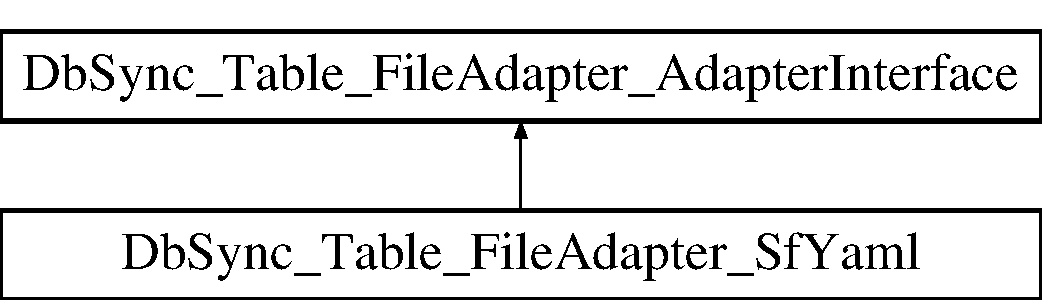
\includegraphics[height=2.000000cm]{interfaceDbSync__Table__FileAdapter__AdapterInterface}
\end{center}
\end{figure}
\subsection*{Public Member Functions}
\begin{DoxyCompactItemize}
\item 
\hyperlink{interfaceDbSync__Table__FileAdapter__AdapterInterface_ab7e4e51cda7ec7e3f4d6f7a08d46cdf3}{\_\-\_\-construct} (\$path)
\item 
\hyperlink{interfaceDbSync__Table__FileAdapter__AdapterInterface_ab48aede121ece3b8a121f75256059c03}{write} (\$filename, array \$data)
\item 
\hyperlink{interfaceDbSync__Table__FileAdapter__AdapterInterface_ae8fbf40502449c3c2c7b18df254d9b08}{load} (\$filename)
\item 
\hyperlink{interfaceDbSync__Table__FileAdapter__AdapterInterface_a0dc7093d0ae8db622a56829c8a735cb0}{getTableList} (\$filename)
\item 
\hyperlink{interfaceDbSync__Table__FileAdapter__AdapterInterface_a7fce4705be965d6025345bf6021cb261}{getFilePath} (\$tableName, \$filename, \$trigger=false)
\item 
\hyperlink{interfaceDbSync__Table__FileAdapter__AdapterInterface_acba15be587d37701eabbd701a62aa7d1}{getTableNameByTriggerName} (\$triggerName)
\item 
\hyperlink{interfaceDbSync__Table__FileAdapter__AdapterInterface_adad6d6497dfe3be7924cb84b9ff65fc8}{getTriggerList} ()
\end{DoxyCompactItemize}


\subsection{Constructor \& Destructor Documentation}
\hypertarget{interfaceDbSync__Table__FileAdapter__AdapterInterface_ab7e4e51cda7ec7e3f4d6f7a08d46cdf3}{
\index{DbSync\_\-Table\_\-FileAdapter\_\-AdapterInterface@{DbSync\_\-Table\_\-FileAdapter\_\-AdapterInterface}!\_\-\_\-construct@{\_\-\_\-construct}}
\index{\_\-\_\-construct@{\_\-\_\-construct}!DbSync_Table_FileAdapter_AdapterInterface@{DbSync\_\-Table\_\-FileAdapter\_\-AdapterInterface}}
\subsubsection[{\_\-\_\-construct}]{\setlength{\rightskip}{0pt plus 5cm}DbSync\_\-Table\_\-FileAdapter\_\-AdapterInterface::\_\-\_\-construct (
\begin{DoxyParamCaption}
\item[{\$}]{path}
\end{DoxyParamCaption}
)}}
\label{interfaceDbSync__Table__FileAdapter__AdapterInterface_ab7e4e51cda7ec7e3f4d6f7a08d46cdf3}
Contructor


\begin{DoxyParams}[1]{Parameters}
string & {\em \$path} & \\
\hline
\end{DoxyParams}


Implemented in \hyperlink{classDbSync__Table__FileAdapter__SfYaml_a0db952aba37ea06d1bed4881011307f1}{DbSync\_\-Table\_\-FileAdapter\_\-SfYaml}.



\subsection{Member Function Documentation}
\hypertarget{interfaceDbSync__Table__FileAdapter__AdapterInterface_a7fce4705be965d6025345bf6021cb261}{
\index{DbSync\_\-Table\_\-FileAdapter\_\-AdapterInterface@{DbSync\_\-Table\_\-FileAdapter\_\-AdapterInterface}!getFilePath@{getFilePath}}
\index{getFilePath@{getFilePath}!DbSync_Table_FileAdapter_AdapterInterface@{DbSync\_\-Table\_\-FileAdapter\_\-AdapterInterface}}
\subsubsection[{getFilePath}]{\setlength{\rightskip}{0pt plus 5cm}DbSync\_\-Table\_\-FileAdapter\_\-AdapterInterface::getFilePath (
\begin{DoxyParamCaption}
\item[{\$}]{tableName, }
\item[{\$}]{filename, }
\item[{\$}]{trigger = {\ttfamily false}}
\end{DoxyParamCaption}
)}}
\label{interfaceDbSync__Table__FileAdapter__AdapterInterface_a7fce4705be965d6025345bf6021cb261}
Get config filepath


\begin{DoxyParams}[1]{Parameters}
boolen & {\em \$real} & \\
\hline
\end{DoxyParams}

\begin{DoxyExceptions}{Exceptions}
{\em Exception} & \\
\hline
\end{DoxyExceptions}
\begin{DoxyReturn}{Returns}
string 
\end{DoxyReturn}


Implemented in \hyperlink{classDbSync__Table__FileAdapter__SfYaml_acbd1d98e3183071612a04d29203215d9}{DbSync\_\-Table\_\-FileAdapter\_\-SfYaml}.

\hypertarget{interfaceDbSync__Table__FileAdapter__AdapterInterface_a0dc7093d0ae8db622a56829c8a735cb0}{
\index{DbSync\_\-Table\_\-FileAdapter\_\-AdapterInterface@{DbSync\_\-Table\_\-FileAdapter\_\-AdapterInterface}!getTableList@{getTableList}}
\index{getTableList@{getTableList}!DbSync_Table_FileAdapter_AdapterInterface@{DbSync\_\-Table\_\-FileAdapter\_\-AdapterInterface}}
\subsubsection[{getTableList}]{\setlength{\rightskip}{0pt plus 5cm}DbSync\_\-Table\_\-FileAdapter\_\-AdapterInterface::getTableList (
\begin{DoxyParamCaption}
\item[{\$}]{filename}
\end{DoxyParamCaption}
)}}
\label{interfaceDbSync__Table__FileAdapter__AdapterInterface_a0dc7093d0ae8db622a56829c8a735cb0}
Get data tables list

\begin{DoxyReturn}{Returns}
array 
\end{DoxyReturn}


Implemented in \hyperlink{classDbSync__Table__FileAdapter__SfYaml_af17a46ddc000204d030e5006343a2203}{DbSync\_\-Table\_\-FileAdapter\_\-SfYaml}.

\hypertarget{interfaceDbSync__Table__FileAdapter__AdapterInterface_acba15be587d37701eabbd701a62aa7d1}{
\index{DbSync\_\-Table\_\-FileAdapter\_\-AdapterInterface@{DbSync\_\-Table\_\-FileAdapter\_\-AdapterInterface}!getTableNameByTriggerName@{getTableNameByTriggerName}}
\index{getTableNameByTriggerName@{getTableNameByTriggerName}!DbSync_Table_FileAdapter_AdapterInterface@{DbSync\_\-Table\_\-FileAdapter\_\-AdapterInterface}}
\subsubsection[{getTableNameByTriggerName}]{\setlength{\rightskip}{0pt plus 5cm}DbSync\_\-Table\_\-FileAdapter\_\-AdapterInterface::getTableNameByTriggerName (
\begin{DoxyParamCaption}
\item[{\$}]{triggerName}
\end{DoxyParamCaption}
)}}
\label{interfaceDbSync__Table__FileAdapter__AdapterInterface_acba15be587d37701eabbd701a62aa7d1}
Get tableName by triggerName


\begin{DoxyParams}[1]{Parameters}
string & {\em \$triggerName} & \\
\hline
\end{DoxyParams}
\begin{DoxyReturn}{Returns}
string 
\end{DoxyReturn}


Implemented in \hyperlink{classDbSync__Table__FileAdapter__SfYaml_a360f51573495d1eab1a11c0d4984e44c}{DbSync\_\-Table\_\-FileAdapter\_\-SfYaml}.

\hypertarget{interfaceDbSync__Table__FileAdapter__AdapterInterface_adad6d6497dfe3be7924cb84b9ff65fc8}{
\index{DbSync\_\-Table\_\-FileAdapter\_\-AdapterInterface@{DbSync\_\-Table\_\-FileAdapter\_\-AdapterInterface}!getTriggerList@{getTriggerList}}
\index{getTriggerList@{getTriggerList}!DbSync_Table_FileAdapter_AdapterInterface@{DbSync\_\-Table\_\-FileAdapter\_\-AdapterInterface}}
\subsubsection[{getTriggerList}]{\setlength{\rightskip}{0pt plus 5cm}DbSync\_\-Table\_\-FileAdapter\_\-AdapterInterface::getTriggerList (
\begin{DoxyParamCaption}
{}
\end{DoxyParamCaption}
)}}
\label{interfaceDbSync__Table__FileAdapter__AdapterInterface_adad6d6497dfe3be7924cb84b9ff65fc8}
Get triggers list

\begin{DoxyReturn}{Returns}
array 
\end{DoxyReturn}
\hypertarget{interfaceDbSync__Table__FileAdapter__AdapterInterface_ae8fbf40502449c3c2c7b18df254d9b08}{
\index{DbSync\_\-Table\_\-FileAdapter\_\-AdapterInterface@{DbSync\_\-Table\_\-FileAdapter\_\-AdapterInterface}!load@{load}}
\index{load@{load}!DbSync_Table_FileAdapter_AdapterInterface@{DbSync\_\-Table\_\-FileAdapter\_\-AdapterInterface}}
\subsubsection[{load}]{\setlength{\rightskip}{0pt plus 5cm}DbSync\_\-Table\_\-FileAdapter\_\-AdapterInterface::load (
\begin{DoxyParamCaption}
\item[{\$}]{filename}
\end{DoxyParamCaption}
)}}
\label{interfaceDbSync__Table__FileAdapter__AdapterInterface_ae8fbf40502449c3c2c7b18df254d9b08}
Load data from file


\begin{DoxyParams}[1]{Parameters}
string & {\em \$filename} & \\
\hline
\end{DoxyParams}
\begin{DoxyReturn}{Returns}
array 
\end{DoxyReturn}


Implemented in \hyperlink{classDbSync__Table__FileAdapter__SfYaml_a0154b63bba21856ca41eabb803fc4507}{DbSync\_\-Table\_\-FileAdapter\_\-SfYaml}.

\hypertarget{interfaceDbSync__Table__FileAdapter__AdapterInterface_ab48aede121ece3b8a121f75256059c03}{
\index{DbSync\_\-Table\_\-FileAdapter\_\-AdapterInterface@{DbSync\_\-Table\_\-FileAdapter\_\-AdapterInterface}!write@{write}}
\index{write@{write}!DbSync_Table_FileAdapter_AdapterInterface@{DbSync\_\-Table\_\-FileAdapter\_\-AdapterInterface}}
\subsubsection[{write}]{\setlength{\rightskip}{0pt plus 5cm}DbSync\_\-Table\_\-FileAdapter\_\-AdapterInterface::write (
\begin{DoxyParamCaption}
\item[{\$}]{filename, }
\item[{array \$}]{data}
\end{DoxyParamCaption}
)}}
\label{interfaceDbSync__Table__FileAdapter__AdapterInterface_ab48aede121ece3b8a121f75256059c03}
Write data to file


\begin{DoxyParams}[1]{Parameters}
string & {\em \$filename} & Full path \\
\hline
array & {\em \$data} & \\
\hline
\end{DoxyParams}
\begin{DoxyReturn}{Returns}
int The function returns the number of bytes that were written to the file, or false on failure. 
\end{DoxyReturn}


Implemented in \hyperlink{classDbSync__Table__FileAdapter__SfYaml_aa8caeb02484d82c83c039182835bba36}{DbSync\_\-Table\_\-FileAdapter\_\-SfYaml}.



The documentation for this interface was generated from the following file:\begin{DoxyCompactItemize}
\item 
DbSync/Table/FileAdapter/AdapterInterface.php\end{DoxyCompactItemize}

\hypertarget{classDbSync__Table__FileAdapter__SfYaml}{
\section{DbSync\_\-Table\_\-FileAdapter\_\-SfYaml Class Reference}
\label{classDbSync__Table__FileAdapter__SfYaml}\index{DbSync\_\-Table\_\-FileAdapter\_\-SfYaml@{DbSync\_\-Table\_\-FileAdapter\_\-SfYaml}}
}
Inheritance diagram for DbSync\_\-Table\_\-FileAdapter\_\-SfYaml:\begin{figure}[H]
\begin{center}
\leavevmode
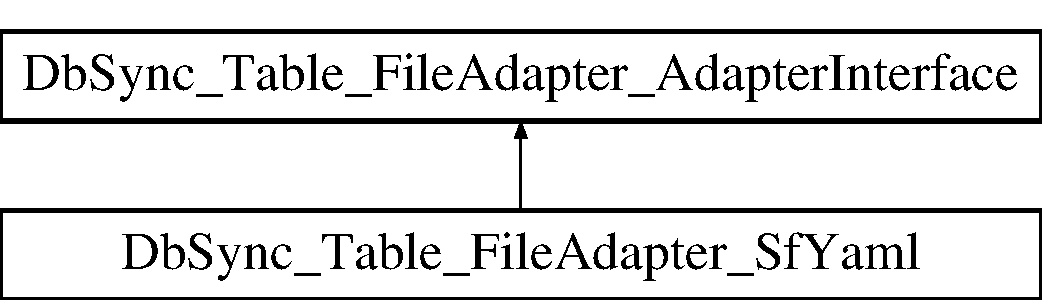
\includegraphics[height=2.000000cm]{classDbSync__Table__FileAdapter__SfYaml}
\end{center}
\end{figure}
\subsection*{Public Member Functions}
\begin{DoxyCompactItemize}
\item 
\hyperlink{classDbSync__Table__FileAdapter__SfYaml_a0db952aba37ea06d1bed4881011307f1}{\_\-\_\-construct} (\$path)
\item 
\hyperlink{classDbSync__Table__FileAdapter__SfYaml_aa8caeb02484d82c83c039182835bba36}{write} (\$filename, array \$data)
\item 
\hyperlink{classDbSync__Table__FileAdapter__SfYaml_a0154b63bba21856ca41eabb803fc4507}{load} (\$filename)
\item 
\hyperlink{classDbSync__Table__FileAdapter__SfYaml_af17a46ddc000204d030e5006343a2203}{getTableList} (\$filename)
\item 
\hyperlink{classDbSync__Table__FileAdapter__SfYaml_acbd1d98e3183071612a04d29203215d9}{getFilePath} (\$tableName, \$filename, \$trigger=false)
\item 
\hyperlink{classDbSync__Table__FileAdapter__SfYaml_a360f51573495d1eab1a11c0d4984e44c}{getTableNameByTriggerName} (\$triggerName)
\item 
\hyperlink{classDbSync__Table__FileAdapter__SfYaml_a3fd272e1ff3162bf1b8decfe5d246103}{getTriggerList} (\$tables=array())
\end{DoxyCompactItemize}
\subsection*{Public Attributes}
\begin{DoxyCompactItemize}
\item 
\hypertarget{classDbSync__Table__FileAdapter__SfYaml_a49fe43bb98940e9b937ccf01d9c078c7}{
const {\bfseries FILE\_\-EXTENSION} = 'yml'}
\label{classDbSync__Table__FileAdapter__SfYaml_a49fe43bb98940e9b937ccf01d9c078c7}

\end{DoxyCompactItemize}
\subsection*{Protected Attributes}
\begin{DoxyCompactItemize}
\item 
\hypertarget{classDbSync__Table__FileAdapter__SfYaml_a11ff7485e50c230488a49d629598c4cd}{
{\bfseries \$\_\-path}}
\label{classDbSync__Table__FileAdapter__SfYaml_a11ff7485e50c230488a49d629598c4cd}

\end{DoxyCompactItemize}


\subsection{Constructor \& Destructor Documentation}
\hypertarget{classDbSync__Table__FileAdapter__SfYaml_a0db952aba37ea06d1bed4881011307f1}{
\index{DbSync\_\-Table\_\-FileAdapter\_\-SfYaml@{DbSync\_\-Table\_\-FileAdapter\_\-SfYaml}!\_\-\_\-construct@{\_\-\_\-construct}}
\index{\_\-\_\-construct@{\_\-\_\-construct}!DbSync_Table_FileAdapter_SfYaml@{DbSync\_\-Table\_\-FileAdapter\_\-SfYaml}}
\subsubsection[{\_\-\_\-construct}]{\setlength{\rightskip}{0pt plus 5cm}DbSync\_\-Table\_\-FileAdapter\_\-SfYaml::\_\-\_\-construct (
\begin{DoxyParamCaption}
\item[{\$}]{path}
\end{DoxyParamCaption}
)}}
\label{classDbSync__Table__FileAdapter__SfYaml_a0db952aba37ea06d1bed4881011307f1}
Contructor


\begin{DoxyParams}[1]{Parameters}
string & {\em \$path} & \\
\hline
\end{DoxyParams}


Implements \hyperlink{interfaceDbSync__Table__FileAdapter__AdapterInterface_ab7e4e51cda7ec7e3f4d6f7a08d46cdf3}{DbSync\_\-Table\_\-FileAdapter\_\-AdapterInterface}.



\subsection{Member Function Documentation}
\hypertarget{classDbSync__Table__FileAdapter__SfYaml_acbd1d98e3183071612a04d29203215d9}{
\index{DbSync\_\-Table\_\-FileAdapter\_\-SfYaml@{DbSync\_\-Table\_\-FileAdapter\_\-SfYaml}!getFilePath@{getFilePath}}
\index{getFilePath@{getFilePath}!DbSync_Table_FileAdapter_SfYaml@{DbSync\_\-Table\_\-FileAdapter\_\-SfYaml}}
\subsubsection[{getFilePath}]{\setlength{\rightskip}{0pt plus 5cm}DbSync\_\-Table\_\-FileAdapter\_\-SfYaml::getFilePath (
\begin{DoxyParamCaption}
\item[{\$}]{tableName, }
\item[{\$}]{filename, }
\item[{\$}]{trigger = {\ttfamily false}}
\end{DoxyParamCaption}
)}}
\label{classDbSync__Table__FileAdapter__SfYaml_acbd1d98e3183071612a04d29203215d9}
Get config filepath


\begin{DoxyParams}[1]{Parameters}
boolen & {\em \$real} & \\
\hline
\end{DoxyParams}

\begin{DoxyExceptions}{Exceptions}
{\em Exception} & \\
\hline
\end{DoxyExceptions}
\begin{DoxyReturn}{Returns}
string 
\end{DoxyReturn}


Implements \hyperlink{interfaceDbSync__Table__FileAdapter__AdapterInterface_a7fce4705be965d6025345bf6021cb261}{DbSync\_\-Table\_\-FileAdapter\_\-AdapterInterface}.

\hypertarget{classDbSync__Table__FileAdapter__SfYaml_af17a46ddc000204d030e5006343a2203}{
\index{DbSync\_\-Table\_\-FileAdapter\_\-SfYaml@{DbSync\_\-Table\_\-FileAdapter\_\-SfYaml}!getTableList@{getTableList}}
\index{getTableList@{getTableList}!DbSync_Table_FileAdapter_SfYaml@{DbSync\_\-Table\_\-FileAdapter\_\-SfYaml}}
\subsubsection[{getTableList}]{\setlength{\rightskip}{0pt plus 5cm}DbSync\_\-Table\_\-FileAdapter\_\-SfYaml::getTableList (
\begin{DoxyParamCaption}
\item[{\$}]{filename}
\end{DoxyParamCaption}
)}}
\label{classDbSync__Table__FileAdapter__SfYaml_af17a46ddc000204d030e5006343a2203}
Get data tables list

\begin{DoxyReturn}{Returns}
array 
\end{DoxyReturn}


Implements \hyperlink{interfaceDbSync__Table__FileAdapter__AdapterInterface_a0dc7093d0ae8db622a56829c8a735cb0}{DbSync\_\-Table\_\-FileAdapter\_\-AdapterInterface}.

\hypertarget{classDbSync__Table__FileAdapter__SfYaml_a360f51573495d1eab1a11c0d4984e44c}{
\index{DbSync\_\-Table\_\-FileAdapter\_\-SfYaml@{DbSync\_\-Table\_\-FileAdapter\_\-SfYaml}!getTableNameByTriggerName@{getTableNameByTriggerName}}
\index{getTableNameByTriggerName@{getTableNameByTriggerName}!DbSync_Table_FileAdapter_SfYaml@{DbSync\_\-Table\_\-FileAdapter\_\-SfYaml}}
\subsubsection[{getTableNameByTriggerName}]{\setlength{\rightskip}{0pt plus 5cm}DbSync\_\-Table\_\-FileAdapter\_\-SfYaml::getTableNameByTriggerName (
\begin{DoxyParamCaption}
\item[{\$}]{triggerName}
\end{DoxyParamCaption}
)}}
\label{classDbSync__Table__FileAdapter__SfYaml_a360f51573495d1eab1a11c0d4984e44c}
Get tableName by triggerName


\begin{DoxyParams}[1]{Parameters}
string & {\em \$triggerName} & \\
\hline
\end{DoxyParams}
\begin{DoxyReturn}{Returns}
string 
\end{DoxyReturn}


Implements \hyperlink{interfaceDbSync__Table__FileAdapter__AdapterInterface_acba15be587d37701eabbd701a62aa7d1}{DbSync\_\-Table\_\-FileAdapter\_\-AdapterInterface}.

\hypertarget{classDbSync__Table__FileAdapter__SfYaml_a3fd272e1ff3162bf1b8decfe5d246103}{
\index{DbSync\_\-Table\_\-FileAdapter\_\-SfYaml@{DbSync\_\-Table\_\-FileAdapter\_\-SfYaml}!getTriggerList@{getTriggerList}}
\index{getTriggerList@{getTriggerList}!DbSync_Table_FileAdapter_SfYaml@{DbSync\_\-Table\_\-FileAdapter\_\-SfYaml}}
\subsubsection[{getTriggerList}]{\setlength{\rightskip}{0pt plus 5cm}DbSync\_\-Table\_\-FileAdapter\_\-SfYaml::getTriggerList (
\begin{DoxyParamCaption}
\item[{\$}]{tables = {\ttfamily array()}}
\end{DoxyParamCaption}
)}}
\label{classDbSync__Table__FileAdapter__SfYaml_a3fd272e1ff3162bf1b8decfe5d246103}
Get triggers list


\begin{DoxyParams}[1]{Parameters}
array & {\em \$tables} & \\
\hline
\end{DoxyParams}
\begin{DoxyReturn}{Returns}
array 
\end{DoxyReturn}
\hypertarget{classDbSync__Table__FileAdapter__SfYaml_a0154b63bba21856ca41eabb803fc4507}{
\index{DbSync\_\-Table\_\-FileAdapter\_\-SfYaml@{DbSync\_\-Table\_\-FileAdapter\_\-SfYaml}!load@{load}}
\index{load@{load}!DbSync_Table_FileAdapter_SfYaml@{DbSync\_\-Table\_\-FileAdapter\_\-SfYaml}}
\subsubsection[{load}]{\setlength{\rightskip}{0pt plus 5cm}DbSync\_\-Table\_\-FileAdapter\_\-SfYaml::load (
\begin{DoxyParamCaption}
\item[{\$}]{filename}
\end{DoxyParamCaption}
)}}
\label{classDbSync__Table__FileAdapter__SfYaml_a0154b63bba21856ca41eabb803fc4507}
Load data from file


\begin{DoxyParams}[1]{Parameters}
string & {\em \$filename} & \\
\hline
\end{DoxyParams}
\begin{DoxyReturn}{Returns}
array 
\end{DoxyReturn}


Implements \hyperlink{interfaceDbSync__Table__FileAdapter__AdapterInterface_ae8fbf40502449c3c2c7b18df254d9b08}{DbSync\_\-Table\_\-FileAdapter\_\-AdapterInterface}.

\hypertarget{classDbSync__Table__FileAdapter__SfYaml_aa8caeb02484d82c83c039182835bba36}{
\index{DbSync\_\-Table\_\-FileAdapter\_\-SfYaml@{DbSync\_\-Table\_\-FileAdapter\_\-SfYaml}!write@{write}}
\index{write@{write}!DbSync_Table_FileAdapter_SfYaml@{DbSync\_\-Table\_\-FileAdapter\_\-SfYaml}}
\subsubsection[{write}]{\setlength{\rightskip}{0pt plus 5cm}DbSync\_\-Table\_\-FileAdapter\_\-SfYaml::write (
\begin{DoxyParamCaption}
\item[{\$}]{filename, }
\item[{array \$}]{data}
\end{DoxyParamCaption}
)}}
\label{classDbSync__Table__FileAdapter__SfYaml_aa8caeb02484d82c83c039182835bba36}
Write data to file


\begin{DoxyParams}[1]{Parameters}
string & {\em \$filename} & Full path \\
\hline
array & {\em \$data} & \\
\hline
\end{DoxyParams}
\begin{DoxyReturn}{Returns}
int The function returns the number of bytes that were written to the file, or false on failure. 
\end{DoxyReturn}


Implements \hyperlink{interfaceDbSync__Table__FileAdapter__AdapterInterface_ab48aede121ece3b8a121f75256059c03}{DbSync\_\-Table\_\-FileAdapter\_\-AdapterInterface}.



The documentation for this class was generated from the following file:\begin{DoxyCompactItemize}
\item 
DbSync/Table/FileAdapter/SfYaml.php\end{DoxyCompactItemize}

\hypertarget{classDbSync__Table__Schema}{
\section{DbSync\_\-Table\_\-Schema Class Reference}
\label{classDbSync__Table__Schema}\index{DbSync\_\-Table\_\-Schema@{DbSync\_\-Table\_\-Schema}}
}
Inheritance diagram for DbSync\_\-Table\_\-Schema:\begin{figure}[H]
\begin{center}
\leavevmode
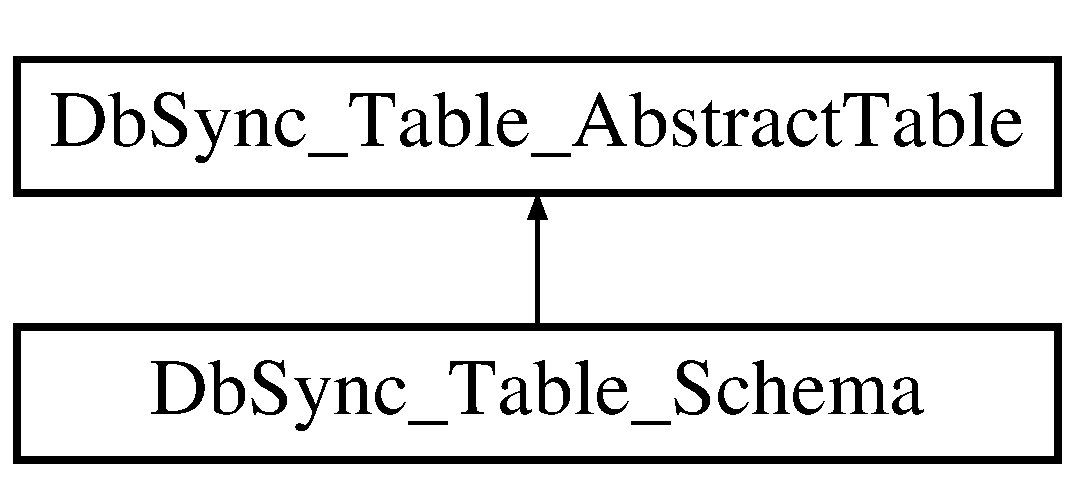
\includegraphics[height=2.000000cm]{classDbSync__Table__Schema}
\end{center}
\end{figure}
\subsection*{Public Member Functions}
\begin{DoxyCompactItemize}
\item 
\hyperlink{classDbSync__Table__Schema_a4e4fa64fe0b799c061f5d9aa8b573085}{getDataToStore} ()
\item 
\hyperlink{classDbSync__Table__Schema_aa50b4443a2c2da1b6c1410c478bce3f2}{createAlter} ()
\item 
\hyperlink{classDbSync__Table__Schema_a697565f517b4bdbd18f74f39b1514d92}{push} ()
\item 
\hyperlink{classDbSync__Table__Schema_a8e963ea0317c5dd9cb11aa34b31cf05a}{dropDbTable} ()
\end{DoxyCompactItemize}
\subsection*{Protected Attributes}
\begin{DoxyCompactItemize}
\item 
\hypertarget{classDbSync__Table__Schema_a118e1c3c58da67335d77c52b4d2192cc}{
{\bfseries \$\_\-filename} = 'schema'}
\label{classDbSync__Table__Schema_a118e1c3c58da67335d77c52b4d2192cc}

\end{DoxyCompactItemize}


\subsection{Member Function Documentation}
\hypertarget{classDbSync__Table__Schema_aa50b4443a2c2da1b6c1410c478bce3f2}{
\index{DbSync\_\-Table\_\-Schema@{DbSync\_\-Table\_\-Schema}!createAlter@{createAlter}}
\index{createAlter@{createAlter}!DbSync_Table_Schema@{DbSync\_\-Table\_\-Schema}}
\subsubsection[{createAlter}]{\setlength{\rightskip}{0pt plus 5cm}DbSync\_\-Table\_\-Schema::createAlter (
\begin{DoxyParamCaption}
{}
\end{DoxyParamCaption}
)}}
\label{classDbSync__Table__Schema_aa50b4443a2c2da1b6c1410c478bce3f2}
Generate Alter Table

\begin{DoxyReturn}{Returns}
string 
\end{DoxyReturn}
\hypertarget{classDbSync__Table__Schema_a8e963ea0317c5dd9cb11aa34b31cf05a}{
\index{DbSync\_\-Table\_\-Schema@{DbSync\_\-Table\_\-Schema}!dropDbTable@{dropDbTable}}
\index{dropDbTable@{dropDbTable}!DbSync_Table_Schema@{DbSync\_\-Table\_\-Schema}}
\subsubsection[{dropDbTable}]{\setlength{\rightskip}{0pt plus 5cm}DbSync\_\-Table\_\-Schema::dropDbTable (
\begin{DoxyParamCaption}
{}
\end{DoxyParamCaption}
)}}
\label{classDbSync__Table__Schema_a8e963ea0317c5dd9cb11aa34b31cf05a}
Delete Table


\begin{DoxyExceptions}{Exceptions}
{\em Exception} & \\
\hline
\end{DoxyExceptions}
\begin{DoxyReturn}{Returns}
boolen 
\end{DoxyReturn}
\hypertarget{classDbSync__Table__Schema_a4e4fa64fe0b799c061f5d9aa8b573085}{
\index{DbSync\_\-Table\_\-Schema@{DbSync\_\-Table\_\-Schema}!getDataToStore@{getDataToStore}}
\index{getDataToStore@{getDataToStore}!DbSync_Table_Schema@{DbSync\_\-Table\_\-Schema}}
\subsubsection[{getDataToStore}]{\setlength{\rightskip}{0pt plus 5cm}DbSync\_\-Table\_\-Schema::getDataToStore (
\begin{DoxyParamCaption}
{}
\end{DoxyParamCaption}
)}}
\label{classDbSync__Table__Schema_a4e4fa64fe0b799c061f5d9aa8b573085}
Get data to store in config file

\begin{DoxyReturn}{Returns}
array 
\end{DoxyReturn}
\hypertarget{classDbSync__Table__Schema_a697565f517b4bdbd18f74f39b1514d92}{
\index{DbSync\_\-Table\_\-Schema@{DbSync\_\-Table\_\-Schema}!push@{push}}
\index{push@{push}!DbSync_Table_Schema@{DbSync\_\-Table\_\-Schema}}
\subsubsection[{push}]{\setlength{\rightskip}{0pt plus 5cm}DbSync\_\-Table\_\-Schema::push (
\begin{DoxyParamCaption}
{}
\end{DoxyParamCaption}
)}}
\label{classDbSync__Table__Schema_a697565f517b4bdbd18f74f39b1514d92}
Alter db table

\begin{DoxyReturn}{Returns}
boolen 
\end{DoxyReturn}


The documentation for this class was generated from the following file:\begin{DoxyCompactItemize}
\item 
DbSync/Table/Schema.php\end{DoxyCompactItemize}

\hypertarget{classDbSync__Table__Trigger}{
\section{DbSync\_\-Table\_\-Trigger Class Reference}
\label{classDbSync__Table__Trigger}\index{DbSync\_\-Table\_\-Trigger@{DbSync\_\-Table\_\-Trigger}}
}
Inheritance diagram for DbSync\_\-Table\_\-Trigger:\begin{figure}[H]
\begin{center}
\leavevmode
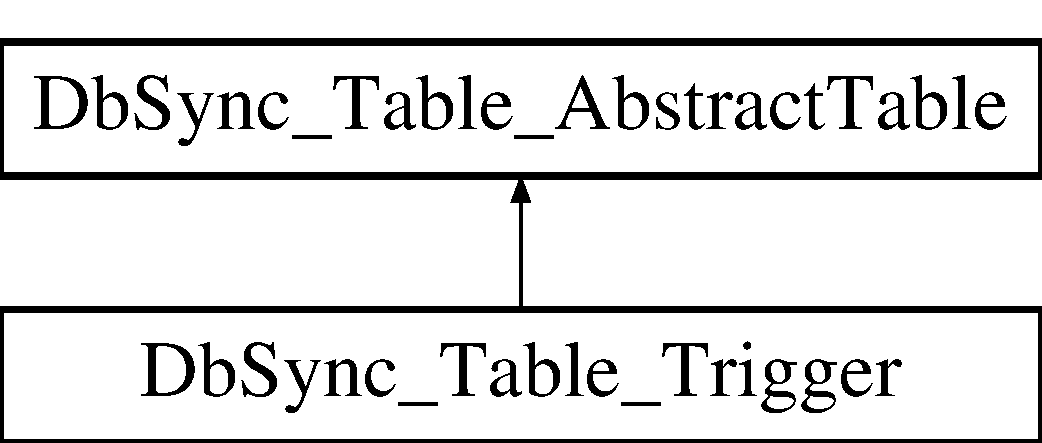
\includegraphics[height=2.000000cm]{classDbSync__Table__Trigger}
\end{center}
\end{figure}
\subsection*{Public Member Functions}
\begin{DoxyCompactItemize}
\item 
\hyperlink{classDbSync__Table__Trigger_a832723eed0417c85bbd318dd275de1c5}{getTriggerName} ()
\item 
\hyperlink{classDbSync__Table__Trigger_a40056b2599be6c972ea953adbecb95da}{setTriggerName} (\$triggerName)
\item 
\hyperlink{classDbSync__Table__Trigger_a2a4c13e2d99327751869644dc053ff85}{getTableName} ()
\item 
\hyperlink{classDbSync__Table__Trigger_a56e0b413a1a52f79f639ba31fa857c55}{getFilePath} (\$real=true)
\item 
\hyperlink{classDbSync__Table__Trigger_a762c5f8968777bfb7cd6cdfeaf068aaf}{getDataToStore} ()
\item 
\hyperlink{classDbSync__Table__Trigger_ad3c52e4ee8319330a1b36fe2e838cf72}{createSql} ()
\item 
\hyperlink{classDbSync__Table__Trigger_a95e1b60f0901dc7a359e76a844f02777}{push} ()
\item 
\hyperlink{classDbSync__Table__Trigger_a88dc54dd7d029b477cbdf5759b4319f3}{dropTrigger} ()
\item 
\hyperlink{classDbSync__Table__Trigger_aa41e17e76ffaa670389421f1f82aa5f7}{getListDb} (\$tables)
\item 
\hyperlink{classDbSync__Table__Trigger_a75499be146da1f7844d1e1d403566c12}{getListConfig} (\$tables)
\item 
\hyperlink{classDbSync__Table__Trigger_a1273b3b648196b339e32a98c58b5ddaa}{getList} (\$tables)
\item 
\hyperlink{classDbSync__Table__Trigger_a6da9349bc4809ef065e6170331544a7f}{hasDbTrigger} ()
\end{DoxyCompactItemize}
\subsection*{Protected Attributes}
\begin{DoxyCompactItemize}
\item 
\hypertarget{classDbSync__Table__Trigger_a5227ca2375c173c79fb4f52a759a59a1}{
{\bfseries \$\_\-triggerName}}
\label{classDbSync__Table__Trigger_a5227ca2375c173c79fb4f52a759a59a1}

\end{DoxyCompactItemize}


\subsection{Member Function Documentation}
\hypertarget{classDbSync__Table__Trigger_ad3c52e4ee8319330a1b36fe2e838cf72}{
\index{DbSync\_\-Table\_\-Trigger@{DbSync\_\-Table\_\-Trigger}!createSql@{createSql}}
\index{createSql@{createSql}!DbSync_Table_Trigger@{DbSync\_\-Table\_\-Trigger}}
\subsubsection[{createSql}]{\setlength{\rightskip}{0pt plus 5cm}DbSync\_\-Table\_\-Trigger::createSql (
\begin{DoxyParamCaption}
{}
\end{DoxyParamCaption}
)}}
\label{classDbSync__Table__Trigger_ad3c52e4ee8319330a1b36fe2e838cf72}
Generate Sql code

\begin{DoxyReturn}{Returns}
string 
\end{DoxyReturn}
\hypertarget{classDbSync__Table__Trigger_a88dc54dd7d029b477cbdf5759b4319f3}{
\index{DbSync\_\-Table\_\-Trigger@{DbSync\_\-Table\_\-Trigger}!dropTrigger@{dropTrigger}}
\index{dropTrigger@{dropTrigger}!DbSync_Table_Trigger@{DbSync\_\-Table\_\-Trigger}}
\subsubsection[{dropTrigger}]{\setlength{\rightskip}{0pt plus 5cm}DbSync\_\-Table\_\-Trigger::dropTrigger (
\begin{DoxyParamCaption}
{}
\end{DoxyParamCaption}
)}}
\label{classDbSync__Table__Trigger_a88dc54dd7d029b477cbdf5759b4319f3}
Delete Table


\begin{DoxyExceptions}{Exceptions}
{\em Exception} & \\
\hline
\end{DoxyExceptions}
\begin{DoxyReturn}{Returns}
boolen 
\end{DoxyReturn}
\hypertarget{classDbSync__Table__Trigger_a762c5f8968777bfb7cd6cdfeaf068aaf}{
\index{DbSync\_\-Table\_\-Trigger@{DbSync\_\-Table\_\-Trigger}!getDataToStore@{getDataToStore}}
\index{getDataToStore@{getDataToStore}!DbSync_Table_Trigger@{DbSync\_\-Table\_\-Trigger}}
\subsubsection[{getDataToStore}]{\setlength{\rightskip}{0pt plus 5cm}DbSync\_\-Table\_\-Trigger::getDataToStore (
\begin{DoxyParamCaption}
{}
\end{DoxyParamCaption}
)}}
\label{classDbSync__Table__Trigger_a762c5f8968777bfb7cd6cdfeaf068aaf}
Get data to store in config file

\begin{DoxyReturn}{Returns}
array 
\end{DoxyReturn}
\hypertarget{classDbSync__Table__Trigger_a56e0b413a1a52f79f639ba31fa857c55}{
\index{DbSync\_\-Table\_\-Trigger@{DbSync\_\-Table\_\-Trigger}!getFilePath@{getFilePath}}
\index{getFilePath@{getFilePath}!DbSync_Table_Trigger@{DbSync\_\-Table\_\-Trigger}}
\subsubsection[{getFilePath}]{\setlength{\rightskip}{0pt plus 5cm}DbSync\_\-Table\_\-Trigger::getFilePath (
\begin{DoxyParamCaption}
\item[{\$}]{real = {\ttfamily true}}
\end{DoxyParamCaption}
)}}
\label{classDbSync__Table__Trigger_a56e0b413a1a52f79f639ba31fa857c55}
Get config filepath


\begin{DoxyParams}[1]{Parameters}
boolen & {\em \$real} & \\
\hline
\end{DoxyParams}

\begin{DoxyExceptions}{Exceptions}
{\em Exception} & \\
\hline
\end{DoxyExceptions}
\begin{DoxyReturn}{Returns}
string 
\end{DoxyReturn}


Reimplemented from \hyperlink{classDbSync__Table__AbstractTable_a69d854fa880beb9ce0a589e0e604c78d}{DbSync\_\-Table\_\-AbstractTable}.

\hypertarget{classDbSync__Table__Trigger_a1273b3b648196b339e32a98c58b5ddaa}{
\index{DbSync\_\-Table\_\-Trigger@{DbSync\_\-Table\_\-Trigger}!getList@{getList}}
\index{getList@{getList}!DbSync_Table_Trigger@{DbSync\_\-Table\_\-Trigger}}
\subsubsection[{getList}]{\setlength{\rightskip}{0pt plus 5cm}DbSync\_\-Table\_\-Trigger::getList (
\begin{DoxyParamCaption}
\item[{\$}]{tables}
\end{DoxyParamCaption}
)}}
\label{classDbSync__Table__Trigger_a1273b3b648196b339e32a98c58b5ddaa}
Get db tables list


\begin{DoxyParams}[1]{Parameters}
array & {\em \$tables} & \\
\hline
\end{DoxyParams}
\begin{DoxyReturn}{Returns}
array 
\end{DoxyReturn}
\hypertarget{classDbSync__Table__Trigger_a75499be146da1f7844d1e1d403566c12}{
\index{DbSync\_\-Table\_\-Trigger@{DbSync\_\-Table\_\-Trigger}!getListConfig@{getListConfig}}
\index{getListConfig@{getListConfig}!DbSync_Table_Trigger@{DbSync\_\-Table\_\-Trigger}}
\subsubsection[{getListConfig}]{\setlength{\rightskip}{0pt plus 5cm}DbSync\_\-Table\_\-Trigger::getListConfig (
\begin{DoxyParamCaption}
\item[{\$}]{tables}
\end{DoxyParamCaption}
)}}
\label{classDbSync__Table__Trigger_a75499be146da1f7844d1e1d403566c12}
Get data tables list


\begin{DoxyParams}[1]{Parameters}
array & {\em \$tables} & \\
\hline
\end{DoxyParams}
\begin{DoxyReturn}{Returns}
array 
\end{DoxyReturn}
\hypertarget{classDbSync__Table__Trigger_aa41e17e76ffaa670389421f1f82aa5f7}{
\index{DbSync\_\-Table\_\-Trigger@{DbSync\_\-Table\_\-Trigger}!getListDb@{getListDb}}
\index{getListDb@{getListDb}!DbSync_Table_Trigger@{DbSync\_\-Table\_\-Trigger}}
\subsubsection[{getListDb}]{\setlength{\rightskip}{0pt plus 5cm}DbSync\_\-Table\_\-Trigger::getListDb (
\begin{DoxyParamCaption}
\item[{\$}]{tables}
\end{DoxyParamCaption}
)}}
\label{classDbSync__Table__Trigger_aa41e17e76ffaa670389421f1f82aa5f7}
Get triggers list


\begin{DoxyParams}[1]{Parameters}
array & {\em \$tables} & \\
\hline
\end{DoxyParams}
\begin{DoxyReturn}{Returns}
array 
\end{DoxyReturn}
\hypertarget{classDbSync__Table__Trigger_a2a4c13e2d99327751869644dc053ff85}{
\index{DbSync\_\-Table\_\-Trigger@{DbSync\_\-Table\_\-Trigger}!getTableName@{getTableName}}
\index{getTableName@{getTableName}!DbSync_Table_Trigger@{DbSync\_\-Table\_\-Trigger}}
\subsubsection[{getTableName}]{\setlength{\rightskip}{0pt plus 5cm}DbSync\_\-Table\_\-Trigger::getTableName (
\begin{DoxyParamCaption}
{}
\end{DoxyParamCaption}
)}}
\label{classDbSync__Table__Trigger_a2a4c13e2d99327751869644dc053ff85}
Get table name

\begin{DoxyReturn}{Returns}
string 
\end{DoxyReturn}


Reimplemented from \hyperlink{classDbSync__Table__AbstractTable_a73bb91b00d38f9653f822ce5f22fdc85}{DbSync\_\-Table\_\-AbstractTable}.

\hypertarget{classDbSync__Table__Trigger_a832723eed0417c85bbd318dd275de1c5}{
\index{DbSync\_\-Table\_\-Trigger@{DbSync\_\-Table\_\-Trigger}!getTriggerName@{getTriggerName}}
\index{getTriggerName@{getTriggerName}!DbSync_Table_Trigger@{DbSync\_\-Table\_\-Trigger}}
\subsubsection[{getTriggerName}]{\setlength{\rightskip}{0pt plus 5cm}DbSync\_\-Table\_\-Trigger::getTriggerName (
\begin{DoxyParamCaption}
{}
\end{DoxyParamCaption}
)}}
\label{classDbSync__Table__Trigger_a832723eed0417c85bbd318dd275de1c5}
Get trigger name

\begin{DoxyReturn}{Returns}
string 
\end{DoxyReturn}
\hypertarget{classDbSync__Table__Trigger_a6da9349bc4809ef065e6170331544a7f}{
\index{DbSync\_\-Table\_\-Trigger@{DbSync\_\-Table\_\-Trigger}!hasDbTrigger@{hasDbTrigger}}
\index{hasDbTrigger@{hasDbTrigger}!DbSync_Table_Trigger@{DbSync\_\-Table\_\-Trigger}}
\subsubsection[{hasDbTrigger}]{\setlength{\rightskip}{0pt plus 5cm}DbSync\_\-Table\_\-Trigger::hasDbTrigger (
\begin{DoxyParamCaption}
{}
\end{DoxyParamCaption}
)}}
\label{classDbSync__Table__Trigger_a6da9349bc4809ef065e6170331544a7f}
Is db table exists

\begin{DoxyReturn}{Returns}
boolen 
\end{DoxyReturn}
\hypertarget{classDbSync__Table__Trigger_a95e1b60f0901dc7a359e76a844f02777}{
\index{DbSync\_\-Table\_\-Trigger@{DbSync\_\-Table\_\-Trigger}!push@{push}}
\index{push@{push}!DbSync_Table_Trigger@{DbSync\_\-Table\_\-Trigger}}
\subsubsection[{push}]{\setlength{\rightskip}{0pt plus 5cm}DbSync\_\-Table\_\-Trigger::push (
\begin{DoxyParamCaption}
{}
\end{DoxyParamCaption}
)}}
\label{classDbSync__Table__Trigger_a95e1b60f0901dc7a359e76a844f02777}
Alter db table

\begin{DoxyReturn}{Returns}
boolen 
\end{DoxyReturn}
\hypertarget{classDbSync__Table__Trigger_a40056b2599be6c972ea953adbecb95da}{
\index{DbSync\_\-Table\_\-Trigger@{DbSync\_\-Table\_\-Trigger}!setTriggerName@{setTriggerName}}
\index{setTriggerName@{setTriggerName}!DbSync_Table_Trigger@{DbSync\_\-Table\_\-Trigger}}
\subsubsection[{setTriggerName}]{\setlength{\rightskip}{0pt plus 5cm}DbSync\_\-Table\_\-Trigger::setTriggerName (
\begin{DoxyParamCaption}
\item[{\$}]{triggerName}
\end{DoxyParamCaption}
)}}
\label{classDbSync__Table__Trigger_a40056b2599be6c972ea953adbecb95da}
Set trigger name


\begin{DoxyParams}[1]{Parameters}
string & {\em \$triggerName} & \\
\hline
\end{DoxyParams}
\begin{DoxyReturn}{Returns}
\hyperlink{namespaceDbSync__Table}{DbSync\_\-Table} 
\end{DoxyReturn}


The documentation for this class was generated from the following file:\begin{DoxyCompactItemize}
\item 
DbSync/Table/Trigger.php\end{DoxyCompactItemize}

\printindex
\end{document}
